\chapter{Część praktyczna}

\section{Problem pomiaru wydajności aplikacji SPA}

\section{Specyfikacja wymagań}

\section{Architektura rozwiązania}
\subsection{Projekt testu wydajności}
\subsection{Budowa aplikacji}
\subsection{Przygotowanie aplikacji do badania}
\subsection{Konteneryzacja aplikacji}
\subsection{Moduł badania}
\subsection{Moduł analizy}

\section{Analiza wyników}
\subsection{Czas załadowania aplikacji}
\subsection{Dodanie 1000 wierszy na początku listy}
\subsection{Dodanie 1000 wierszy na końcu listy}
\subsection{Zamiana wszystkich wierszy na liście}
\subsection{Aktualizacja 500 wierszy}
\subsection{Zamiana miejscami dwóch wierszy}
\subsection{Usunięcie pojedynczego wiersza}
\subsection{Usunięcie wszystkich wierszy}

\begin{figure}[!ht]
    \centering
    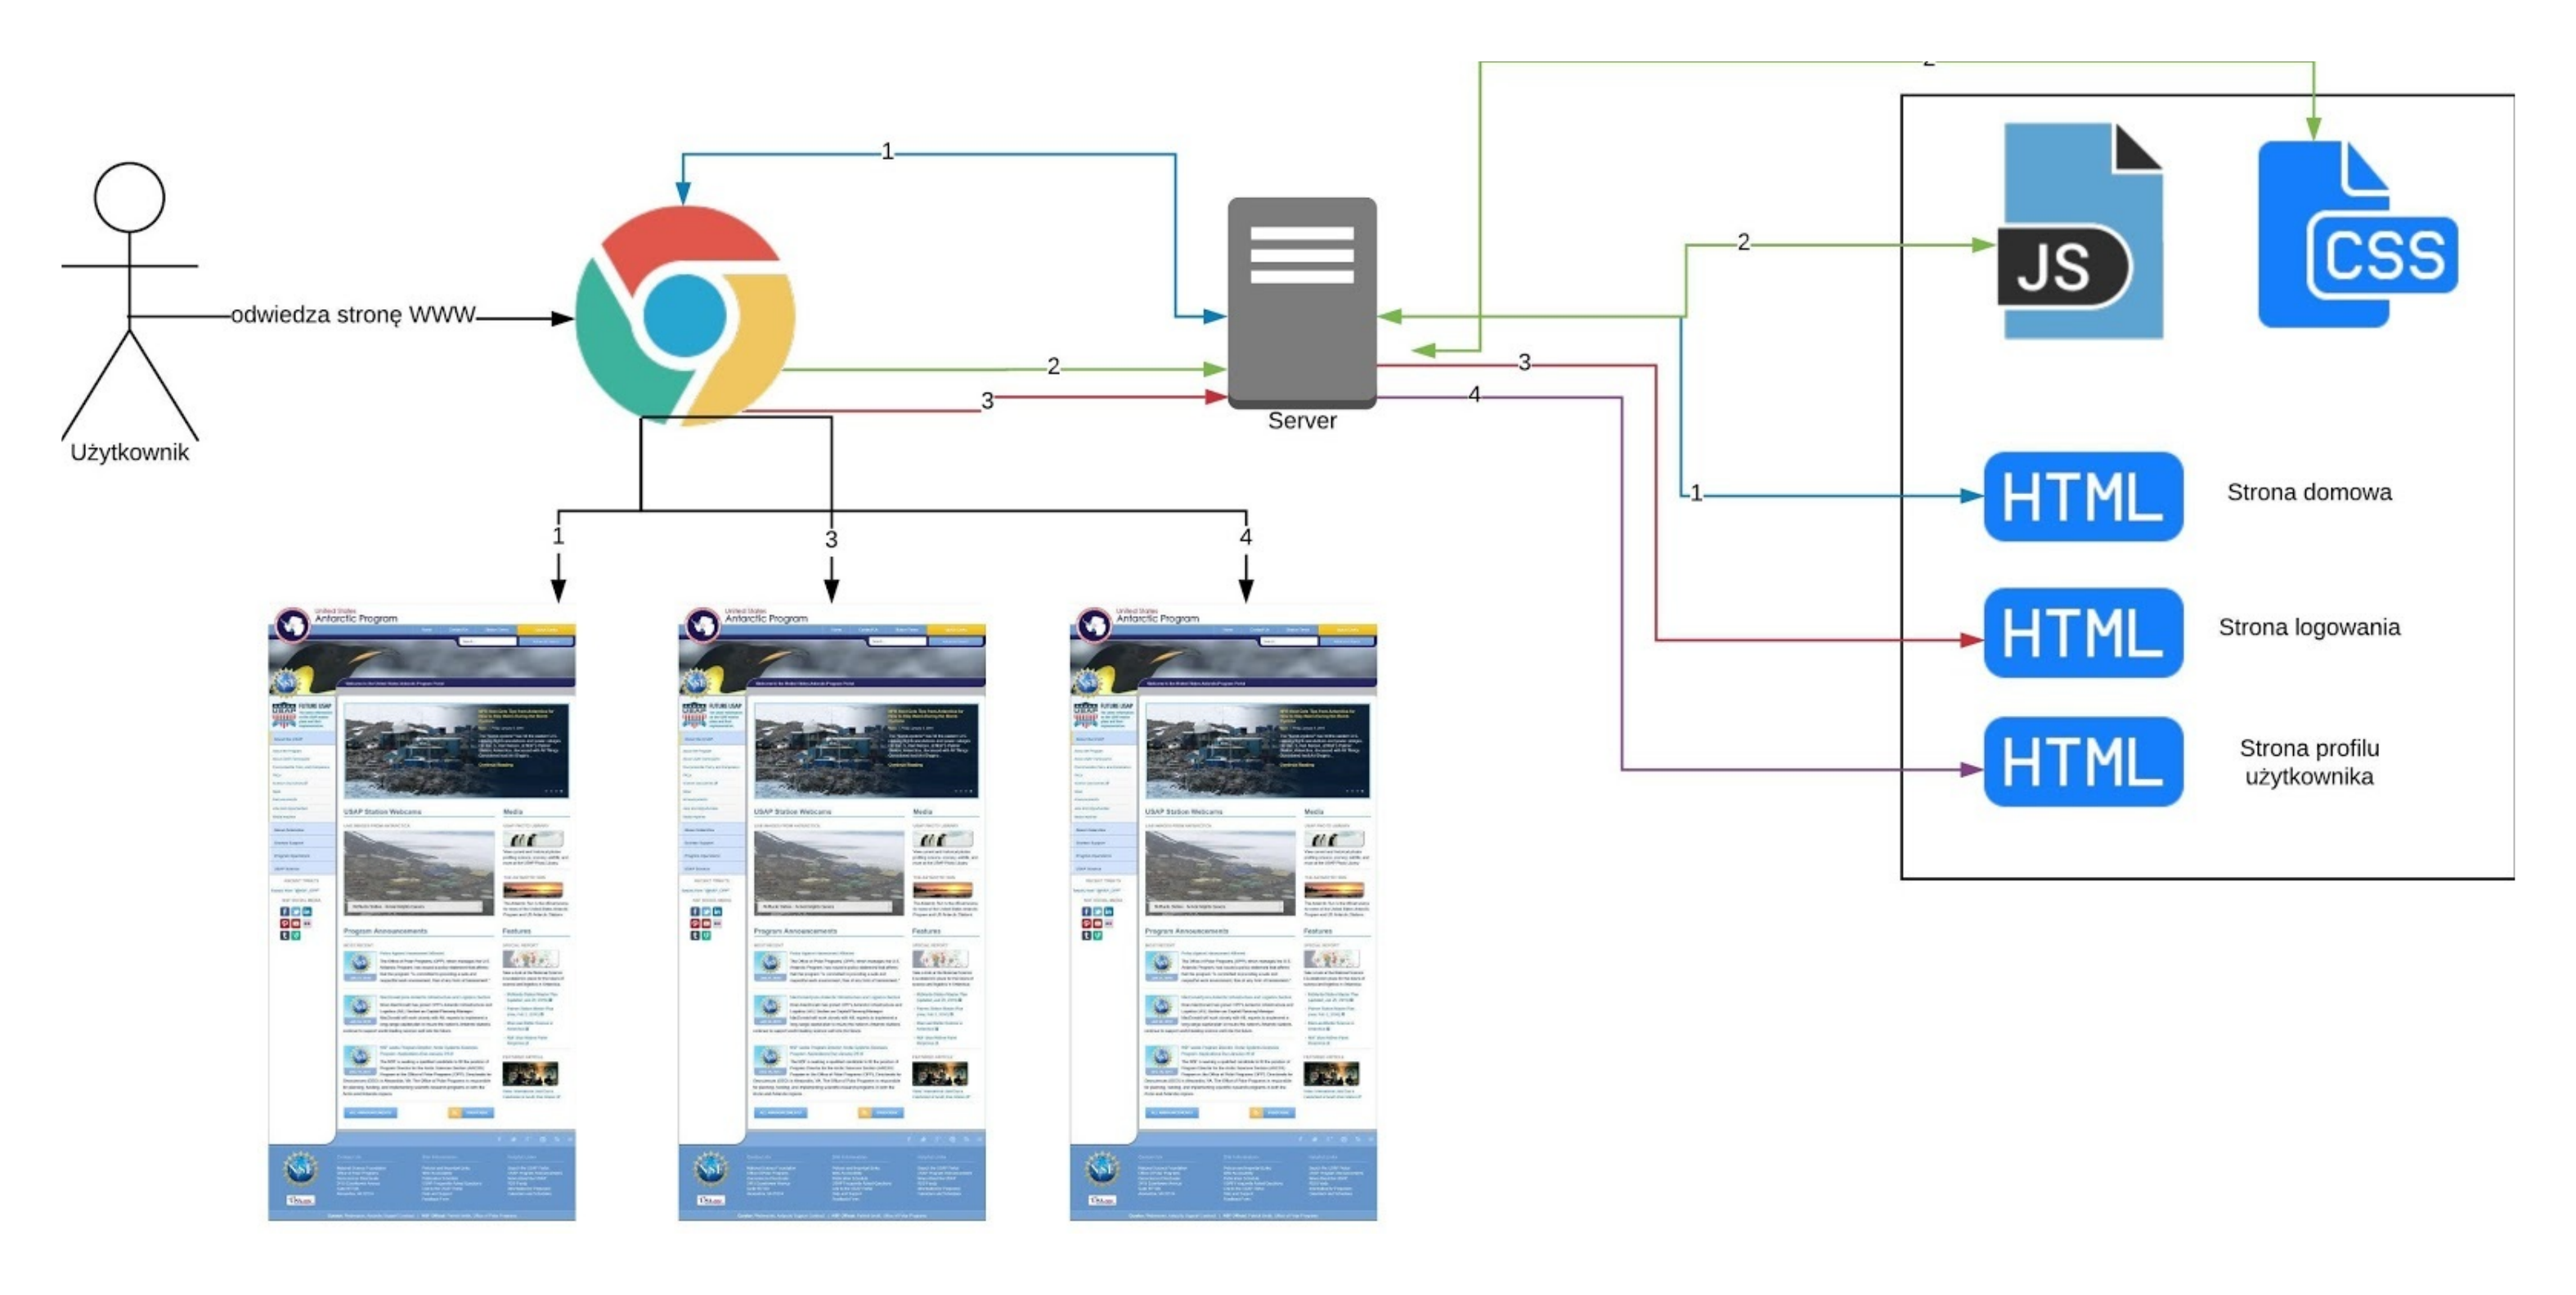
\includegraphics[width=12cm]{rysunek_7.png}
    \caption{Ilustracja przedstawiająca cykl życia statycznej strony internetowej}
    \label{fig:rysunek_7}
\end{figure}

\begin{figure}[!ht]
    \centering
    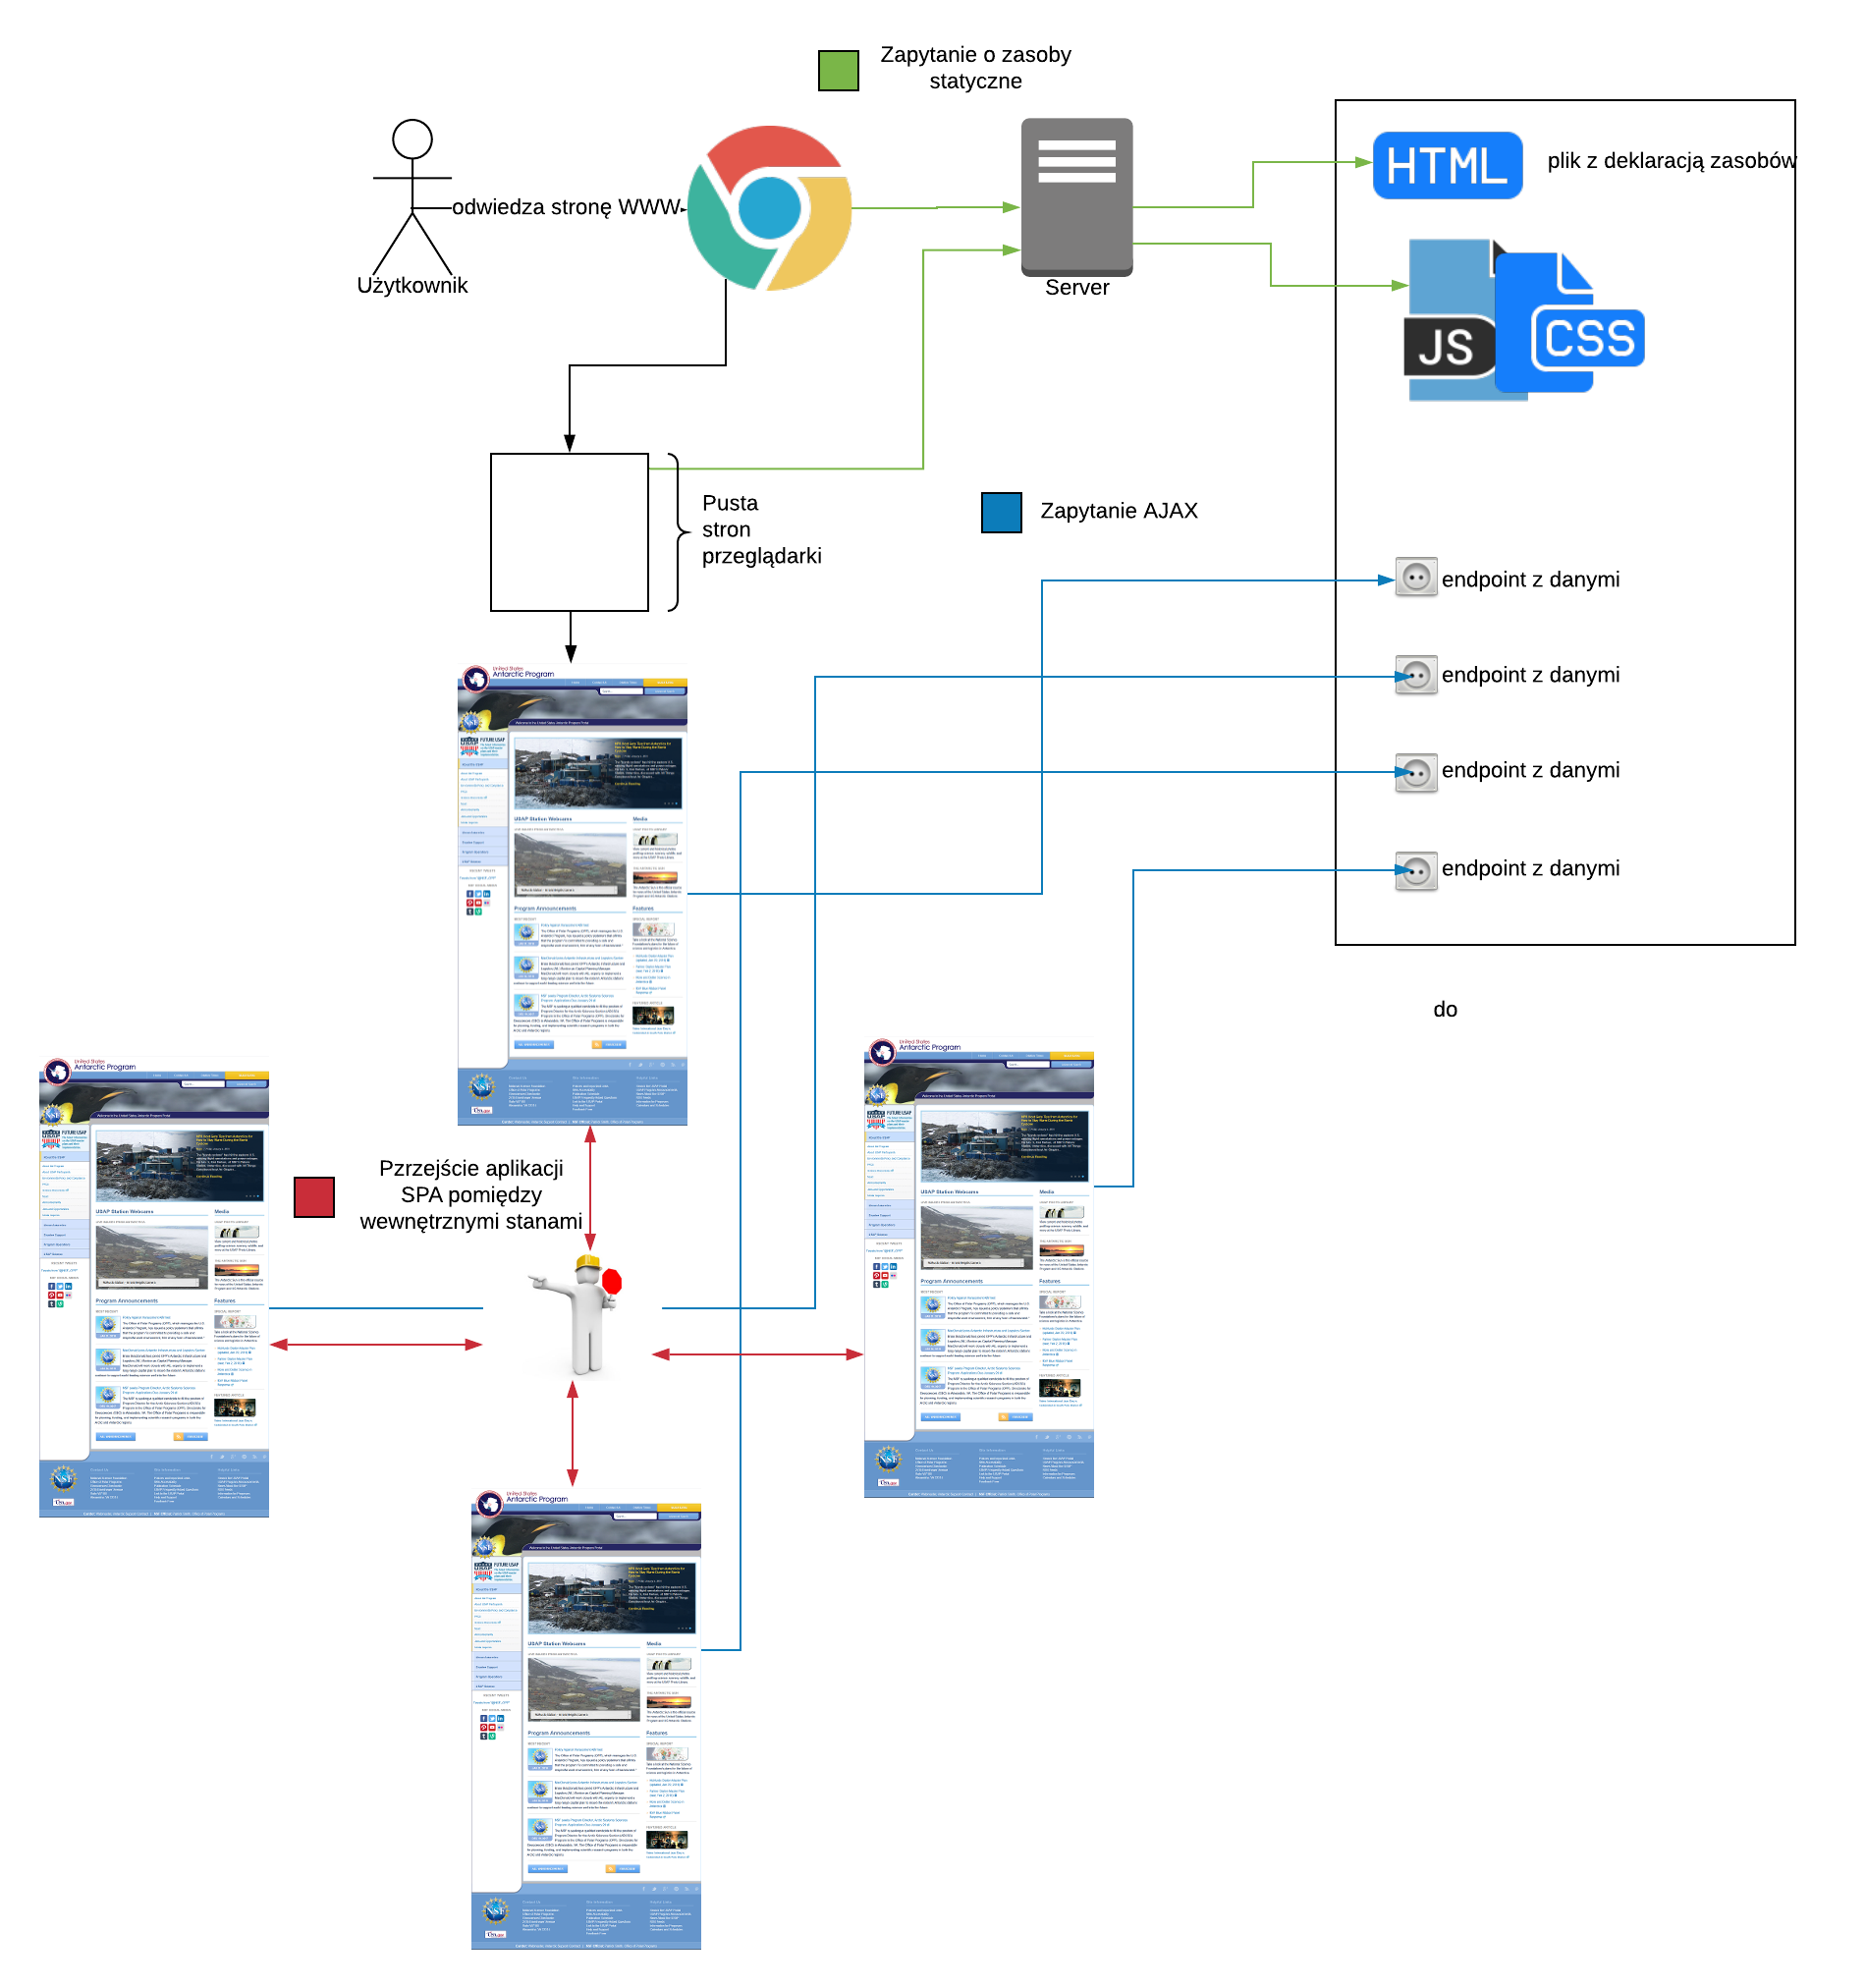
\includegraphics[width=12cm]{rysunek_8.png}
    \caption{Ilustracja przedstawiająca cykl działania aplikacji SPA}
    \label{fig:rysunek_8}
\end{figure}

\begin{figure}[!ht]
    \centering
    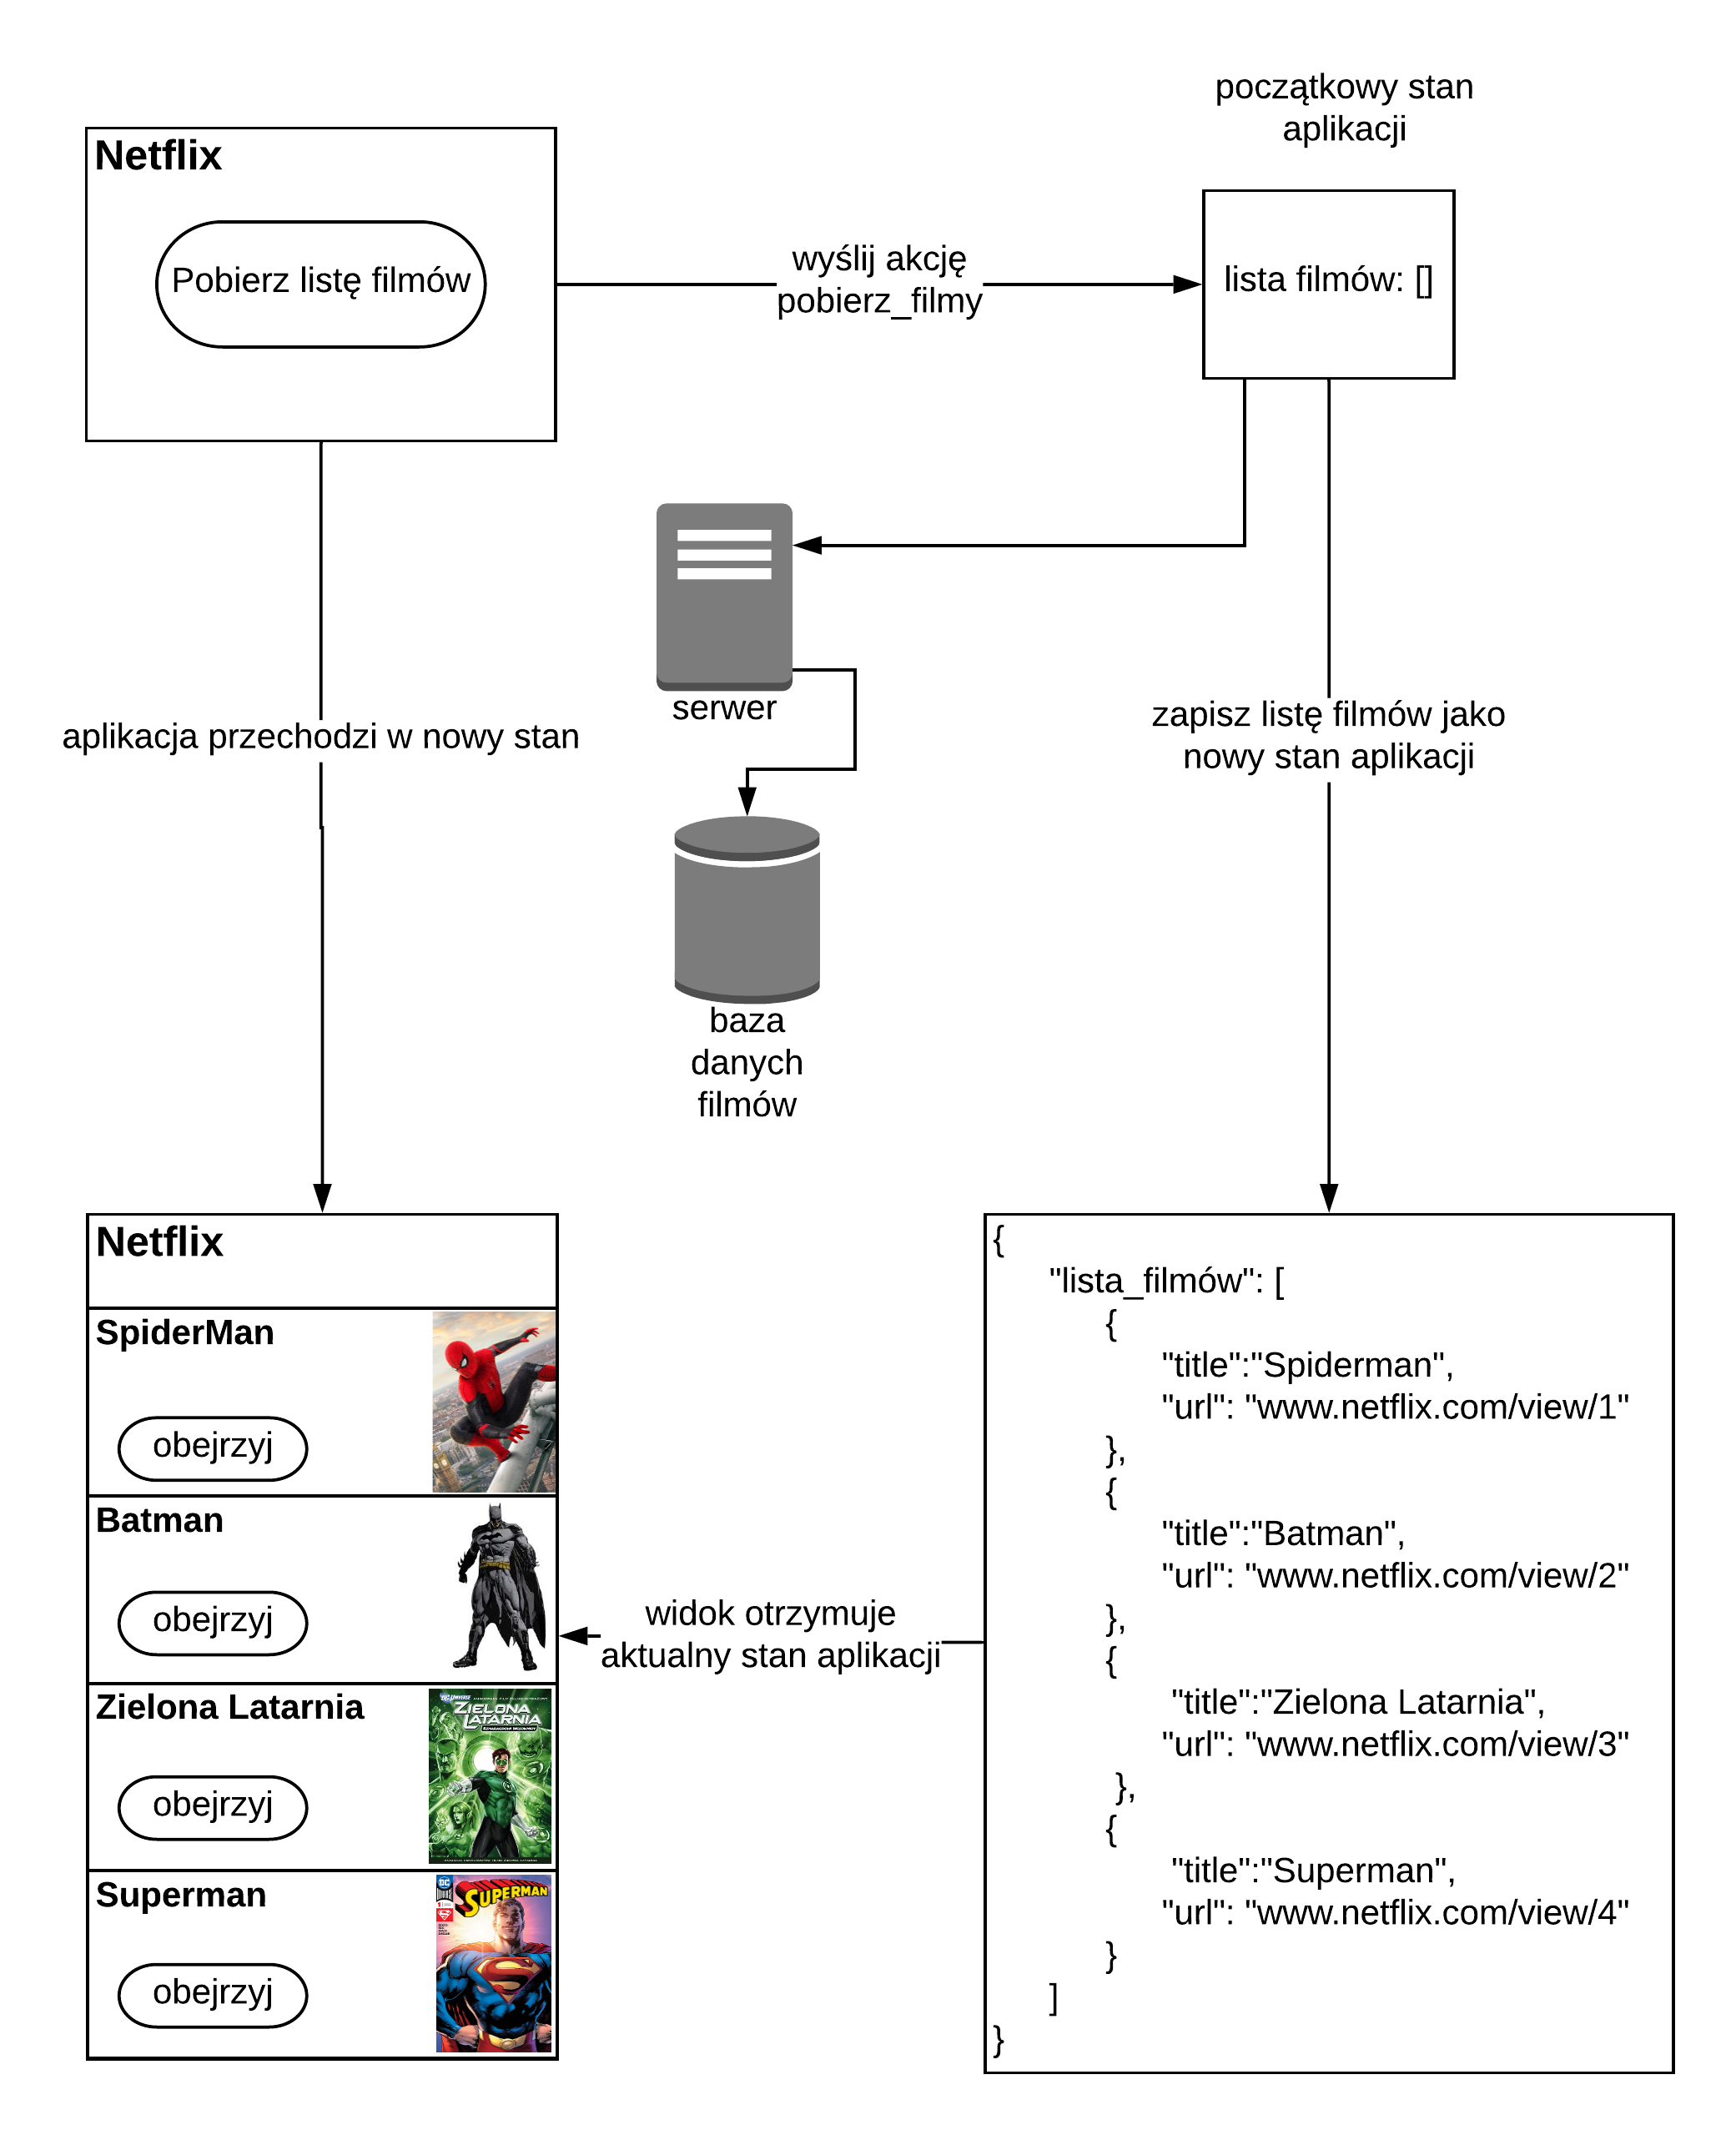
\includegraphics[width=12cm]{rysunek_9.png}
    \caption{Grafika przedstawiająca mechanizm działania aplikacji dynamicznych}
    \label{fig:rysunek_9}
\end{figure}

\begin{figure}[!ht]
    \centering
    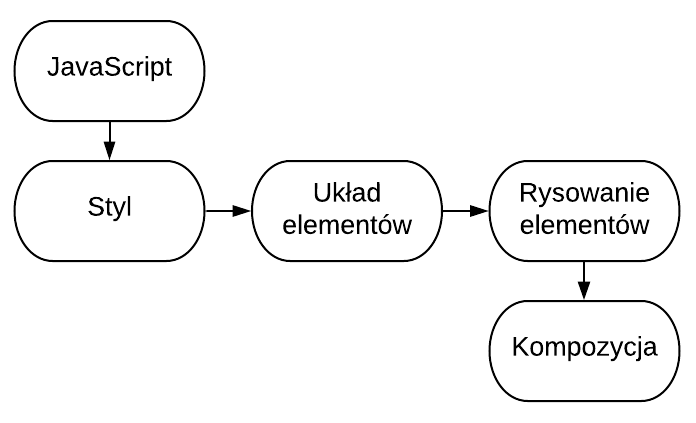
\includegraphics[width=12cm]{rysunek_10.png}
    \caption{Grafika przedstawiająca kolejność faz renderowania w przeglądarce}
    \label{fig:rysunek_10}
\end{figure}

\begin{figure}[!ht]
    \centering
    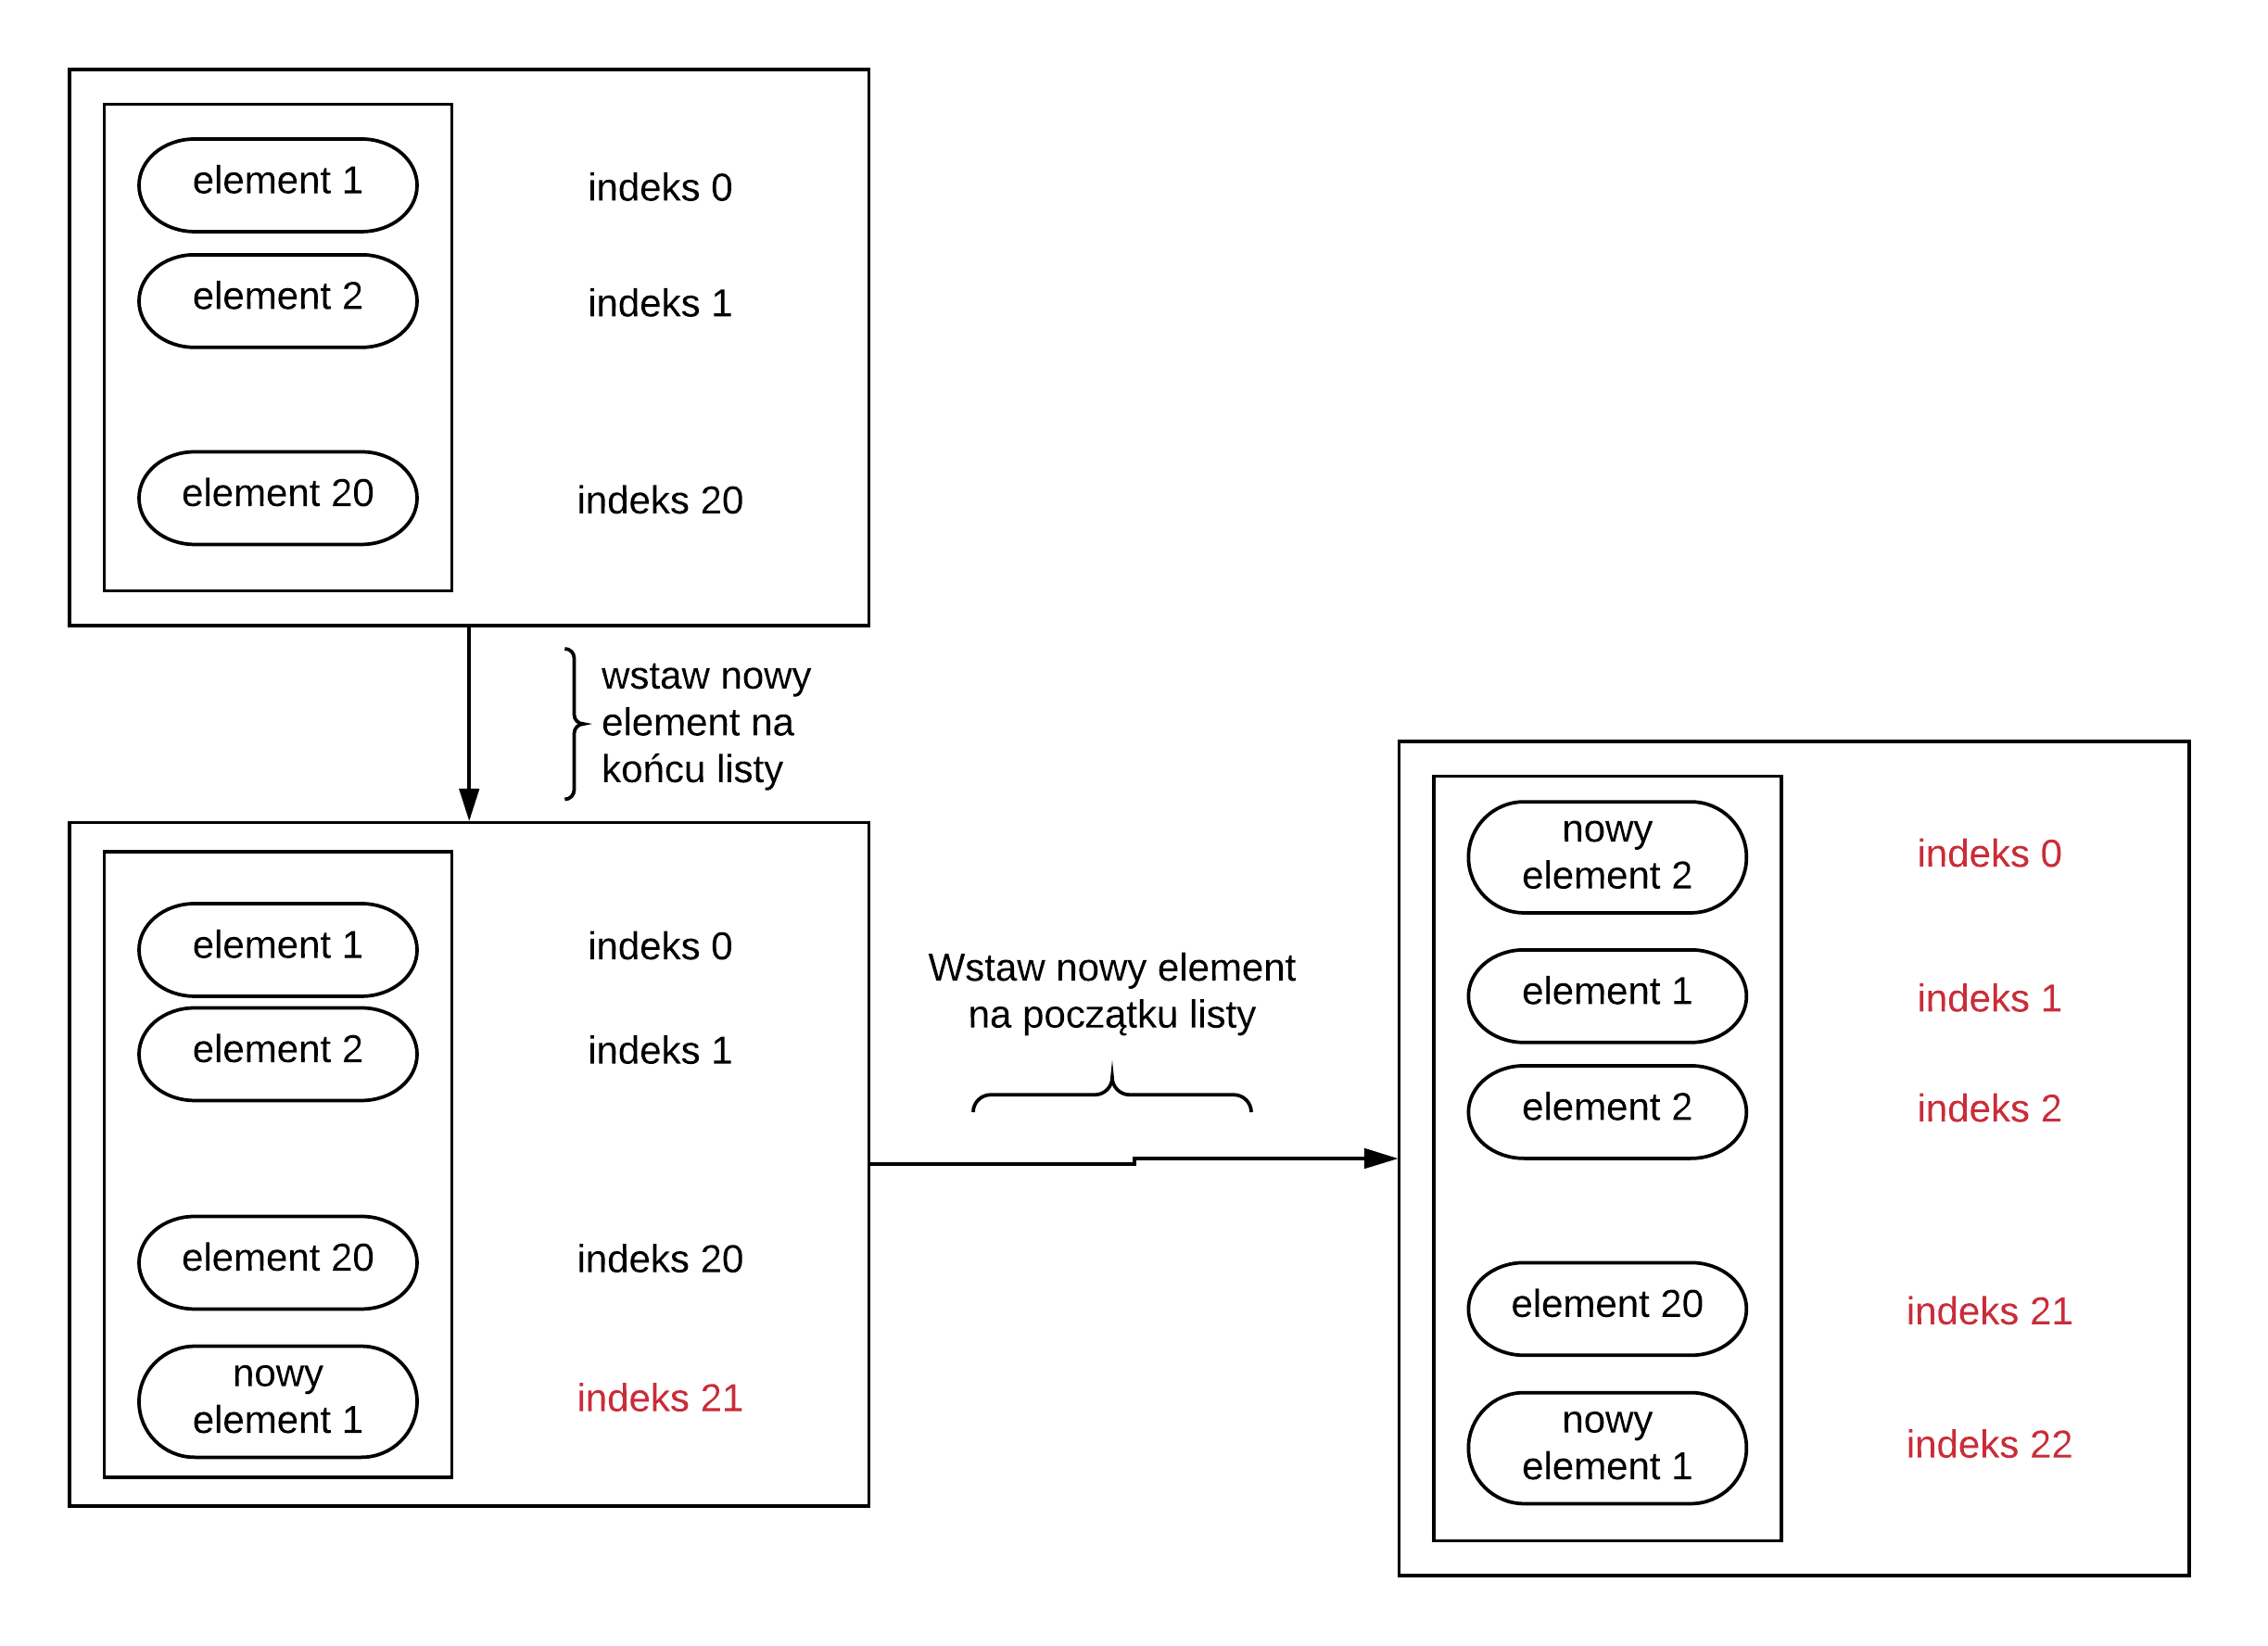
\includegraphics[width=12cm]{rysunek_11.png}
    \caption{Ilustracja przedstawiająca problem dopisywania elementu na koniec listy}
    \label{fig:rysunek_11}
\end{figure}

\begin{figure}[!ht]
    \centering
    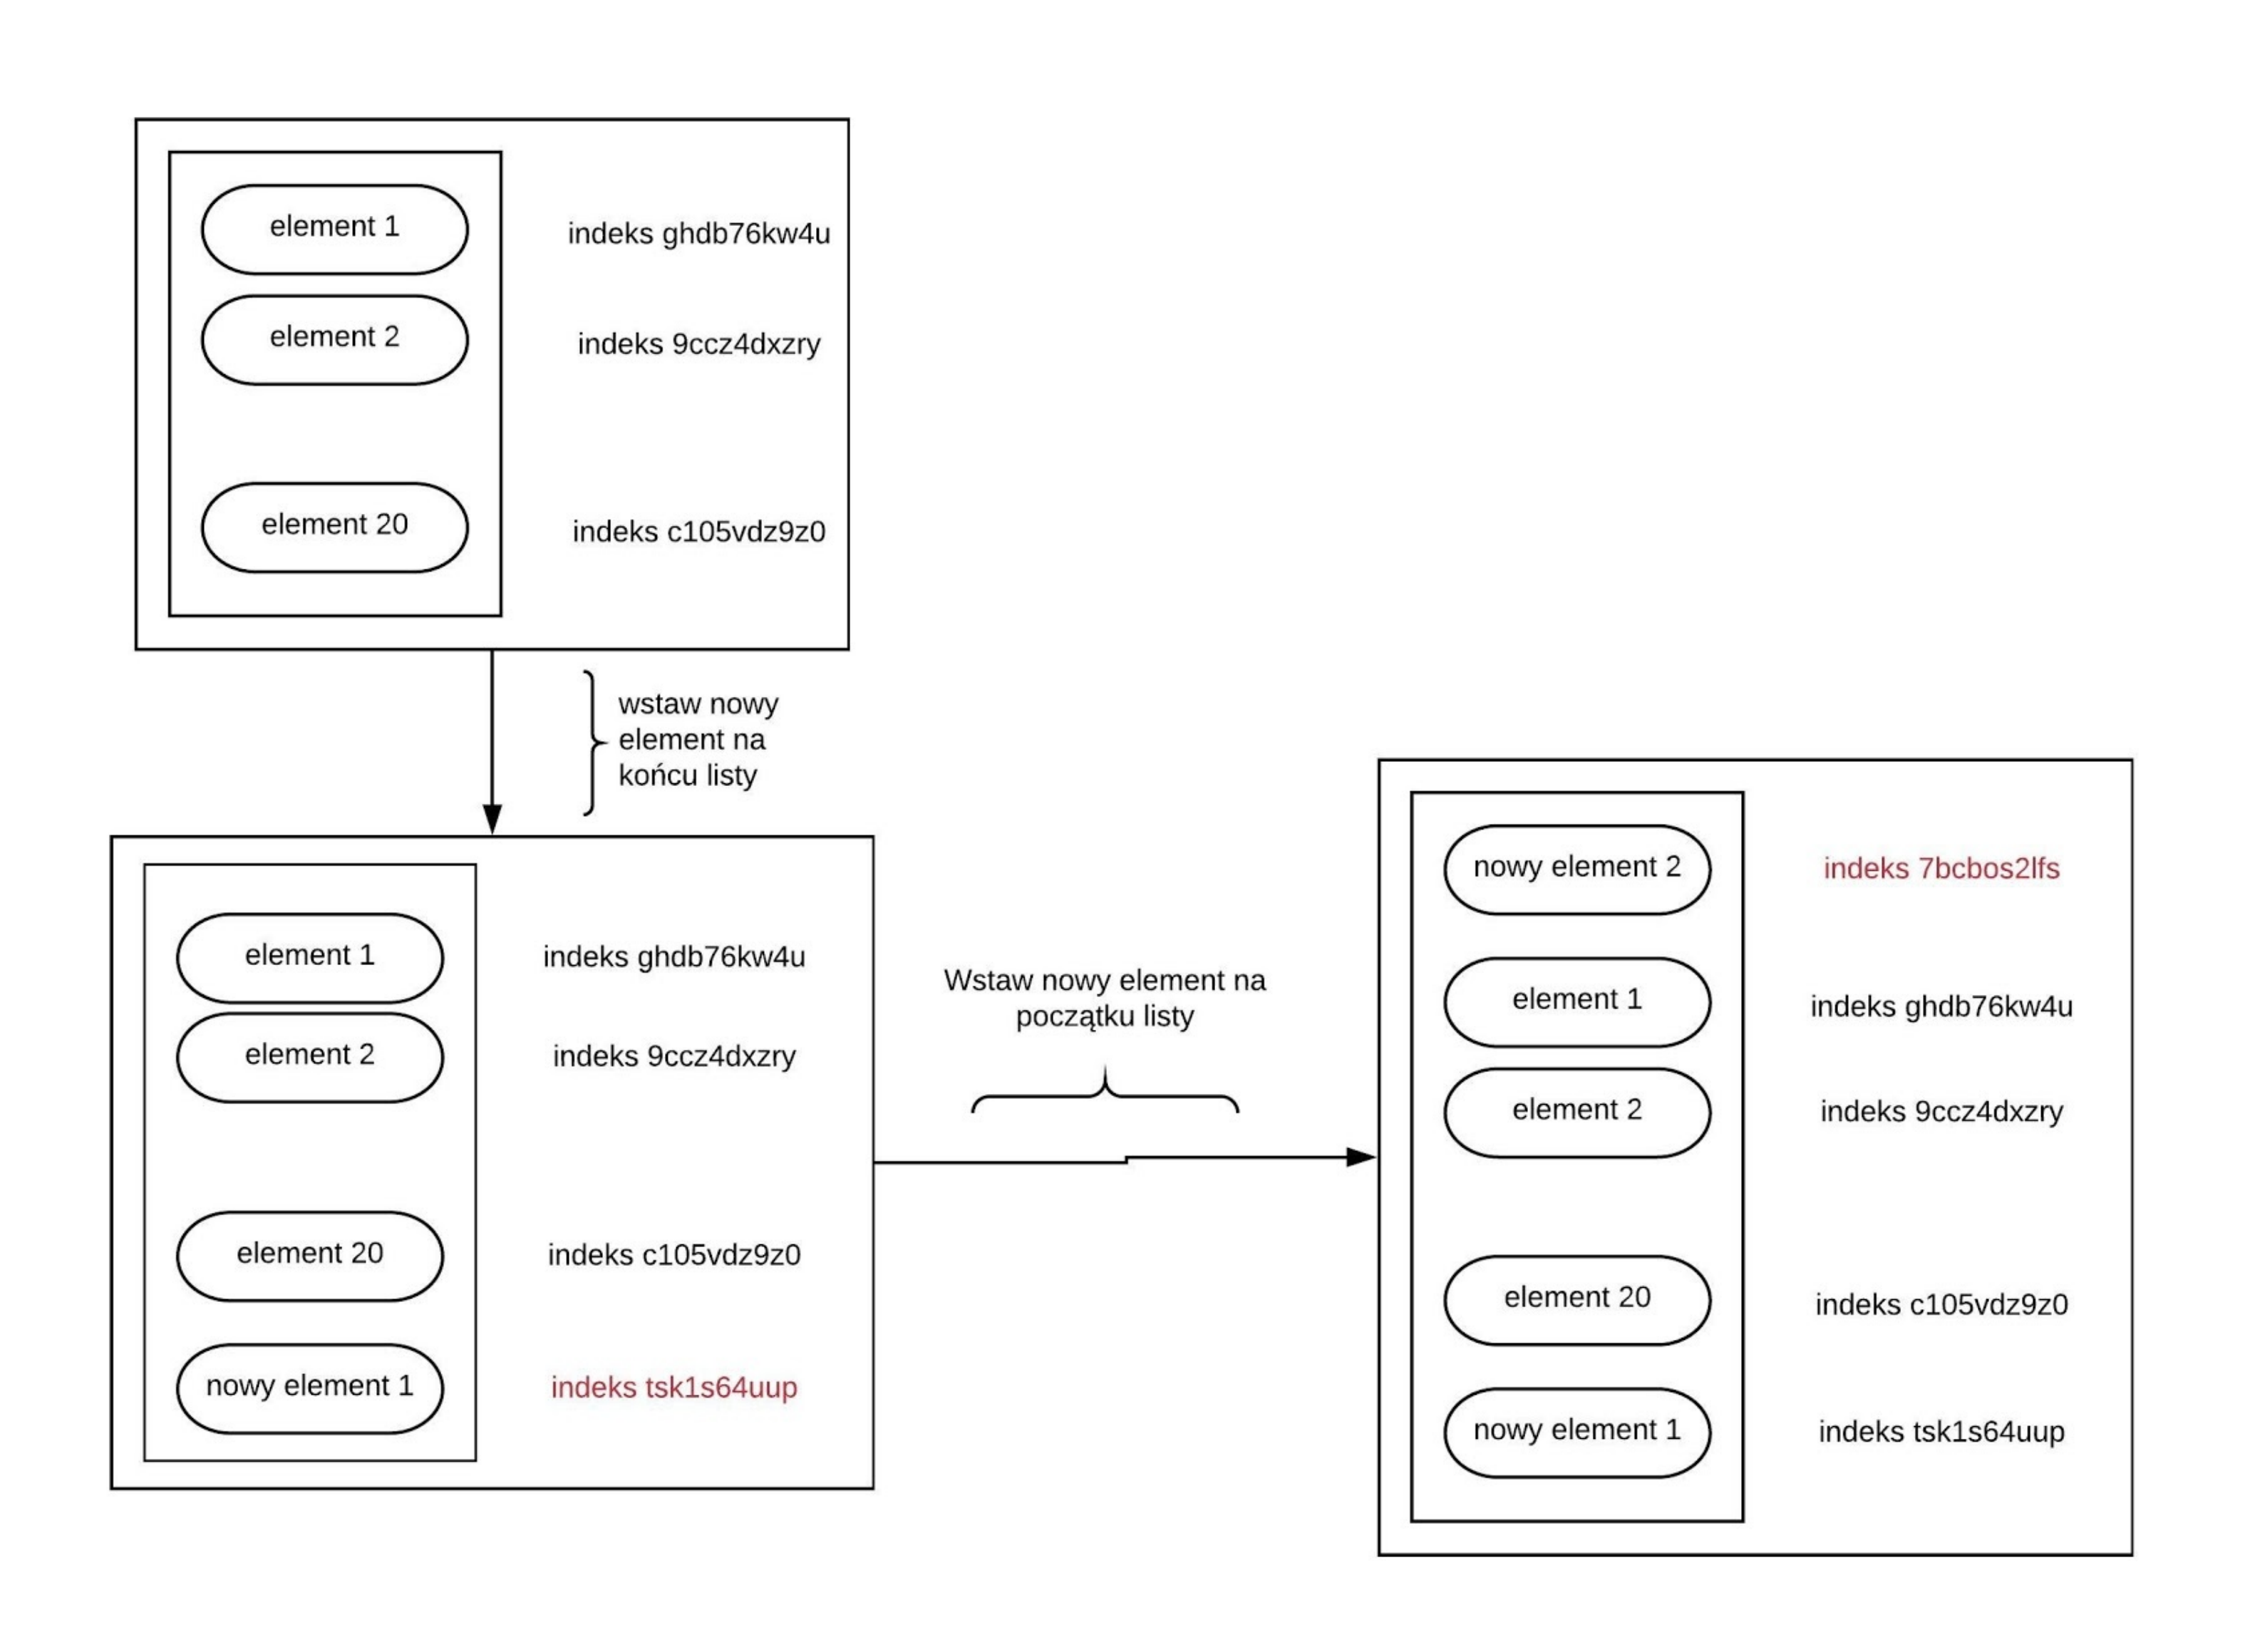
\includegraphics[width=12cm]{rysunek_12.png}
    \caption{Ilustracja przedstawiająca problem dopisywania elementów na początek listy}
    \label{fig:rysunek_12}
\end{figure}

\begin{figure}[!ht]
    \centering
    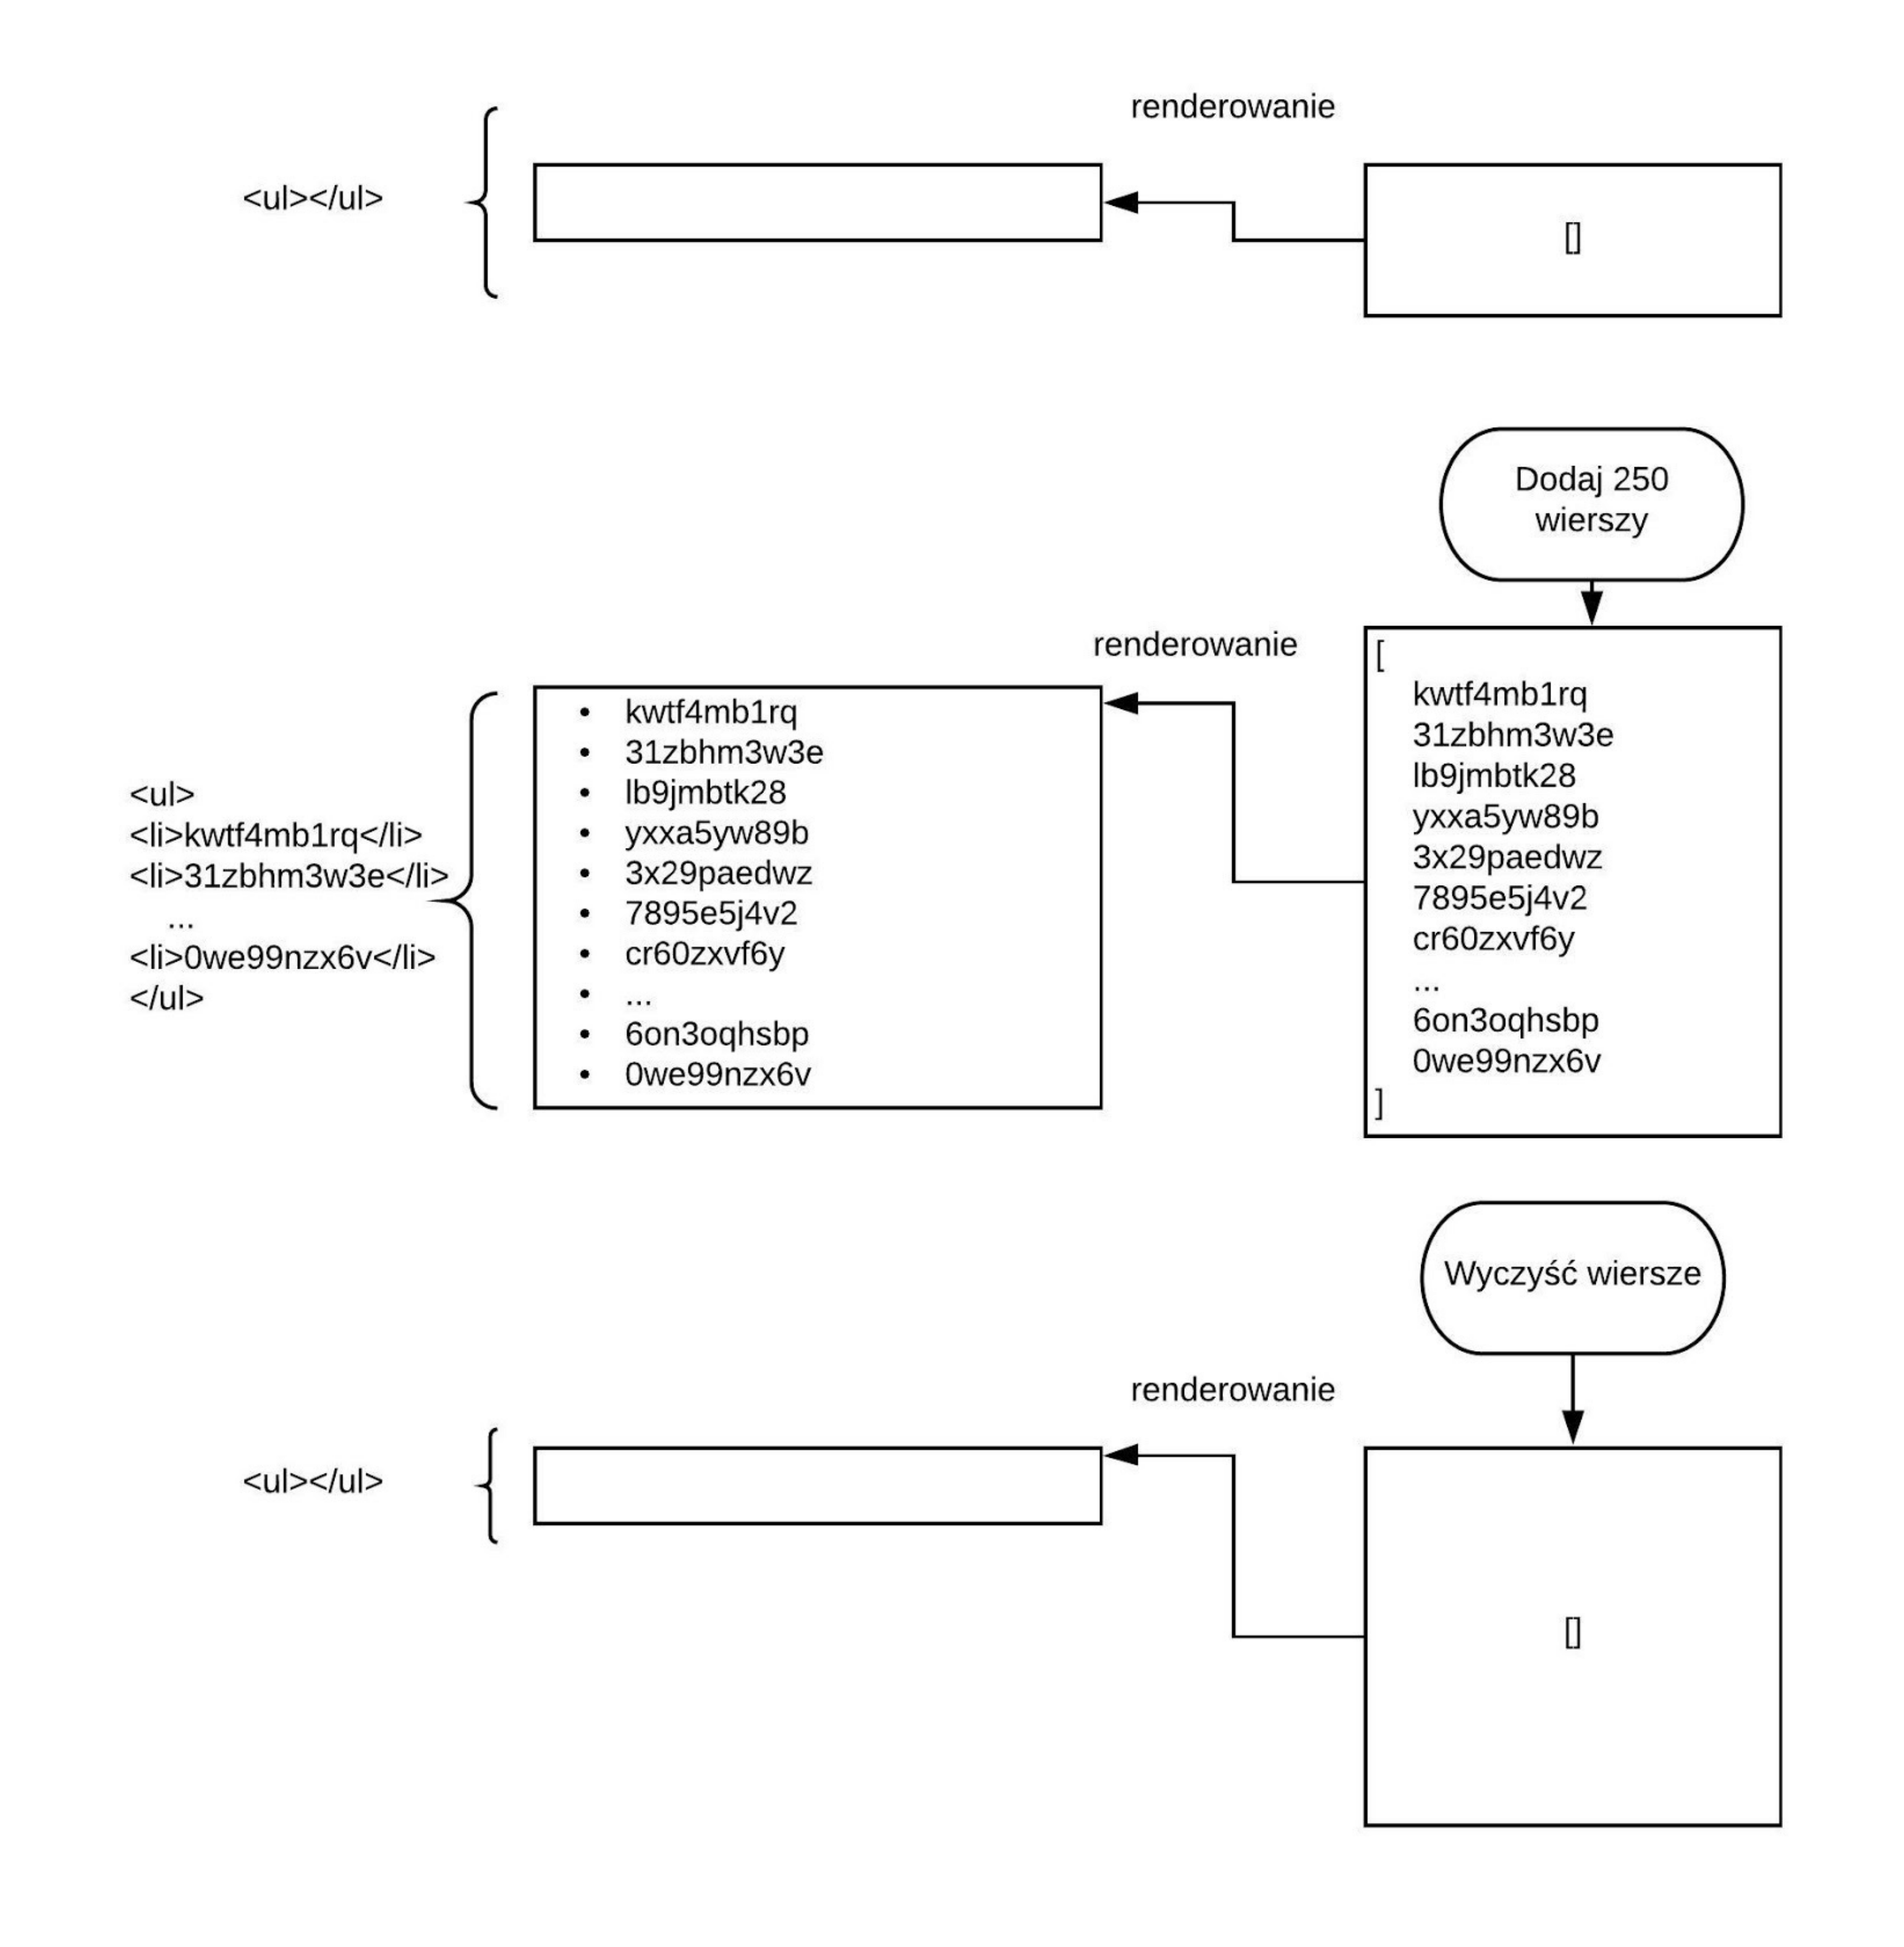
\includegraphics[width=12cm]{rysunek_13.png}
    \caption{Ilustracja mechanizmu przebiegu badania}
    \label{fig:rysunek_13}
\end{figure}

\begin{figure}[!ht]
    \centering
    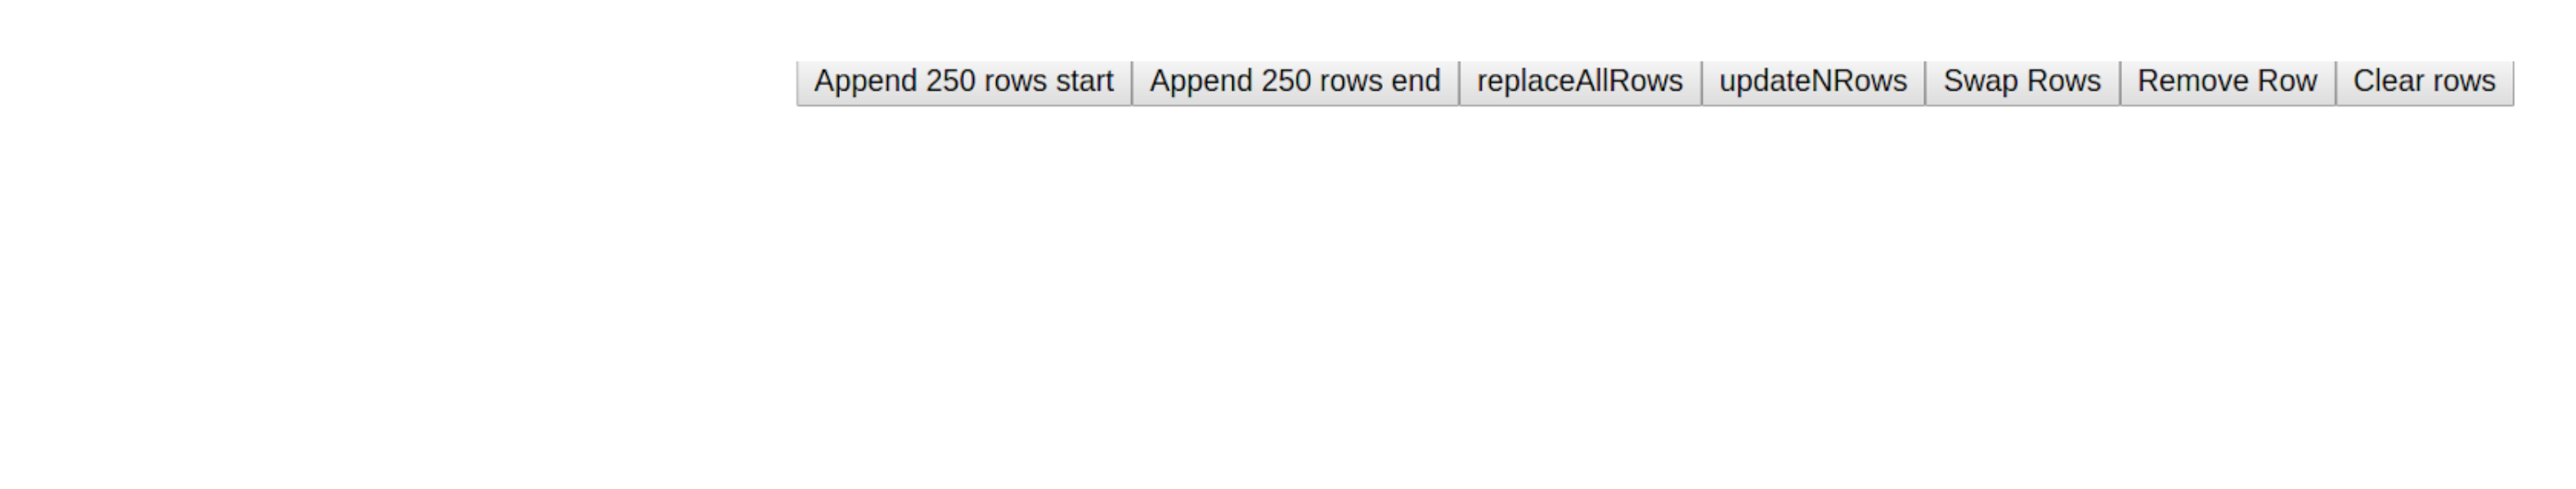
\includegraphics[width=12cm]{rysunek_14.png}
    \caption{Grafika przedstawiająca zaimplementowane przyciski w aplikacji}
    \label{fig:rysunek_14}
\end{figure}

\begin{figure}[!ht]
    \centering
    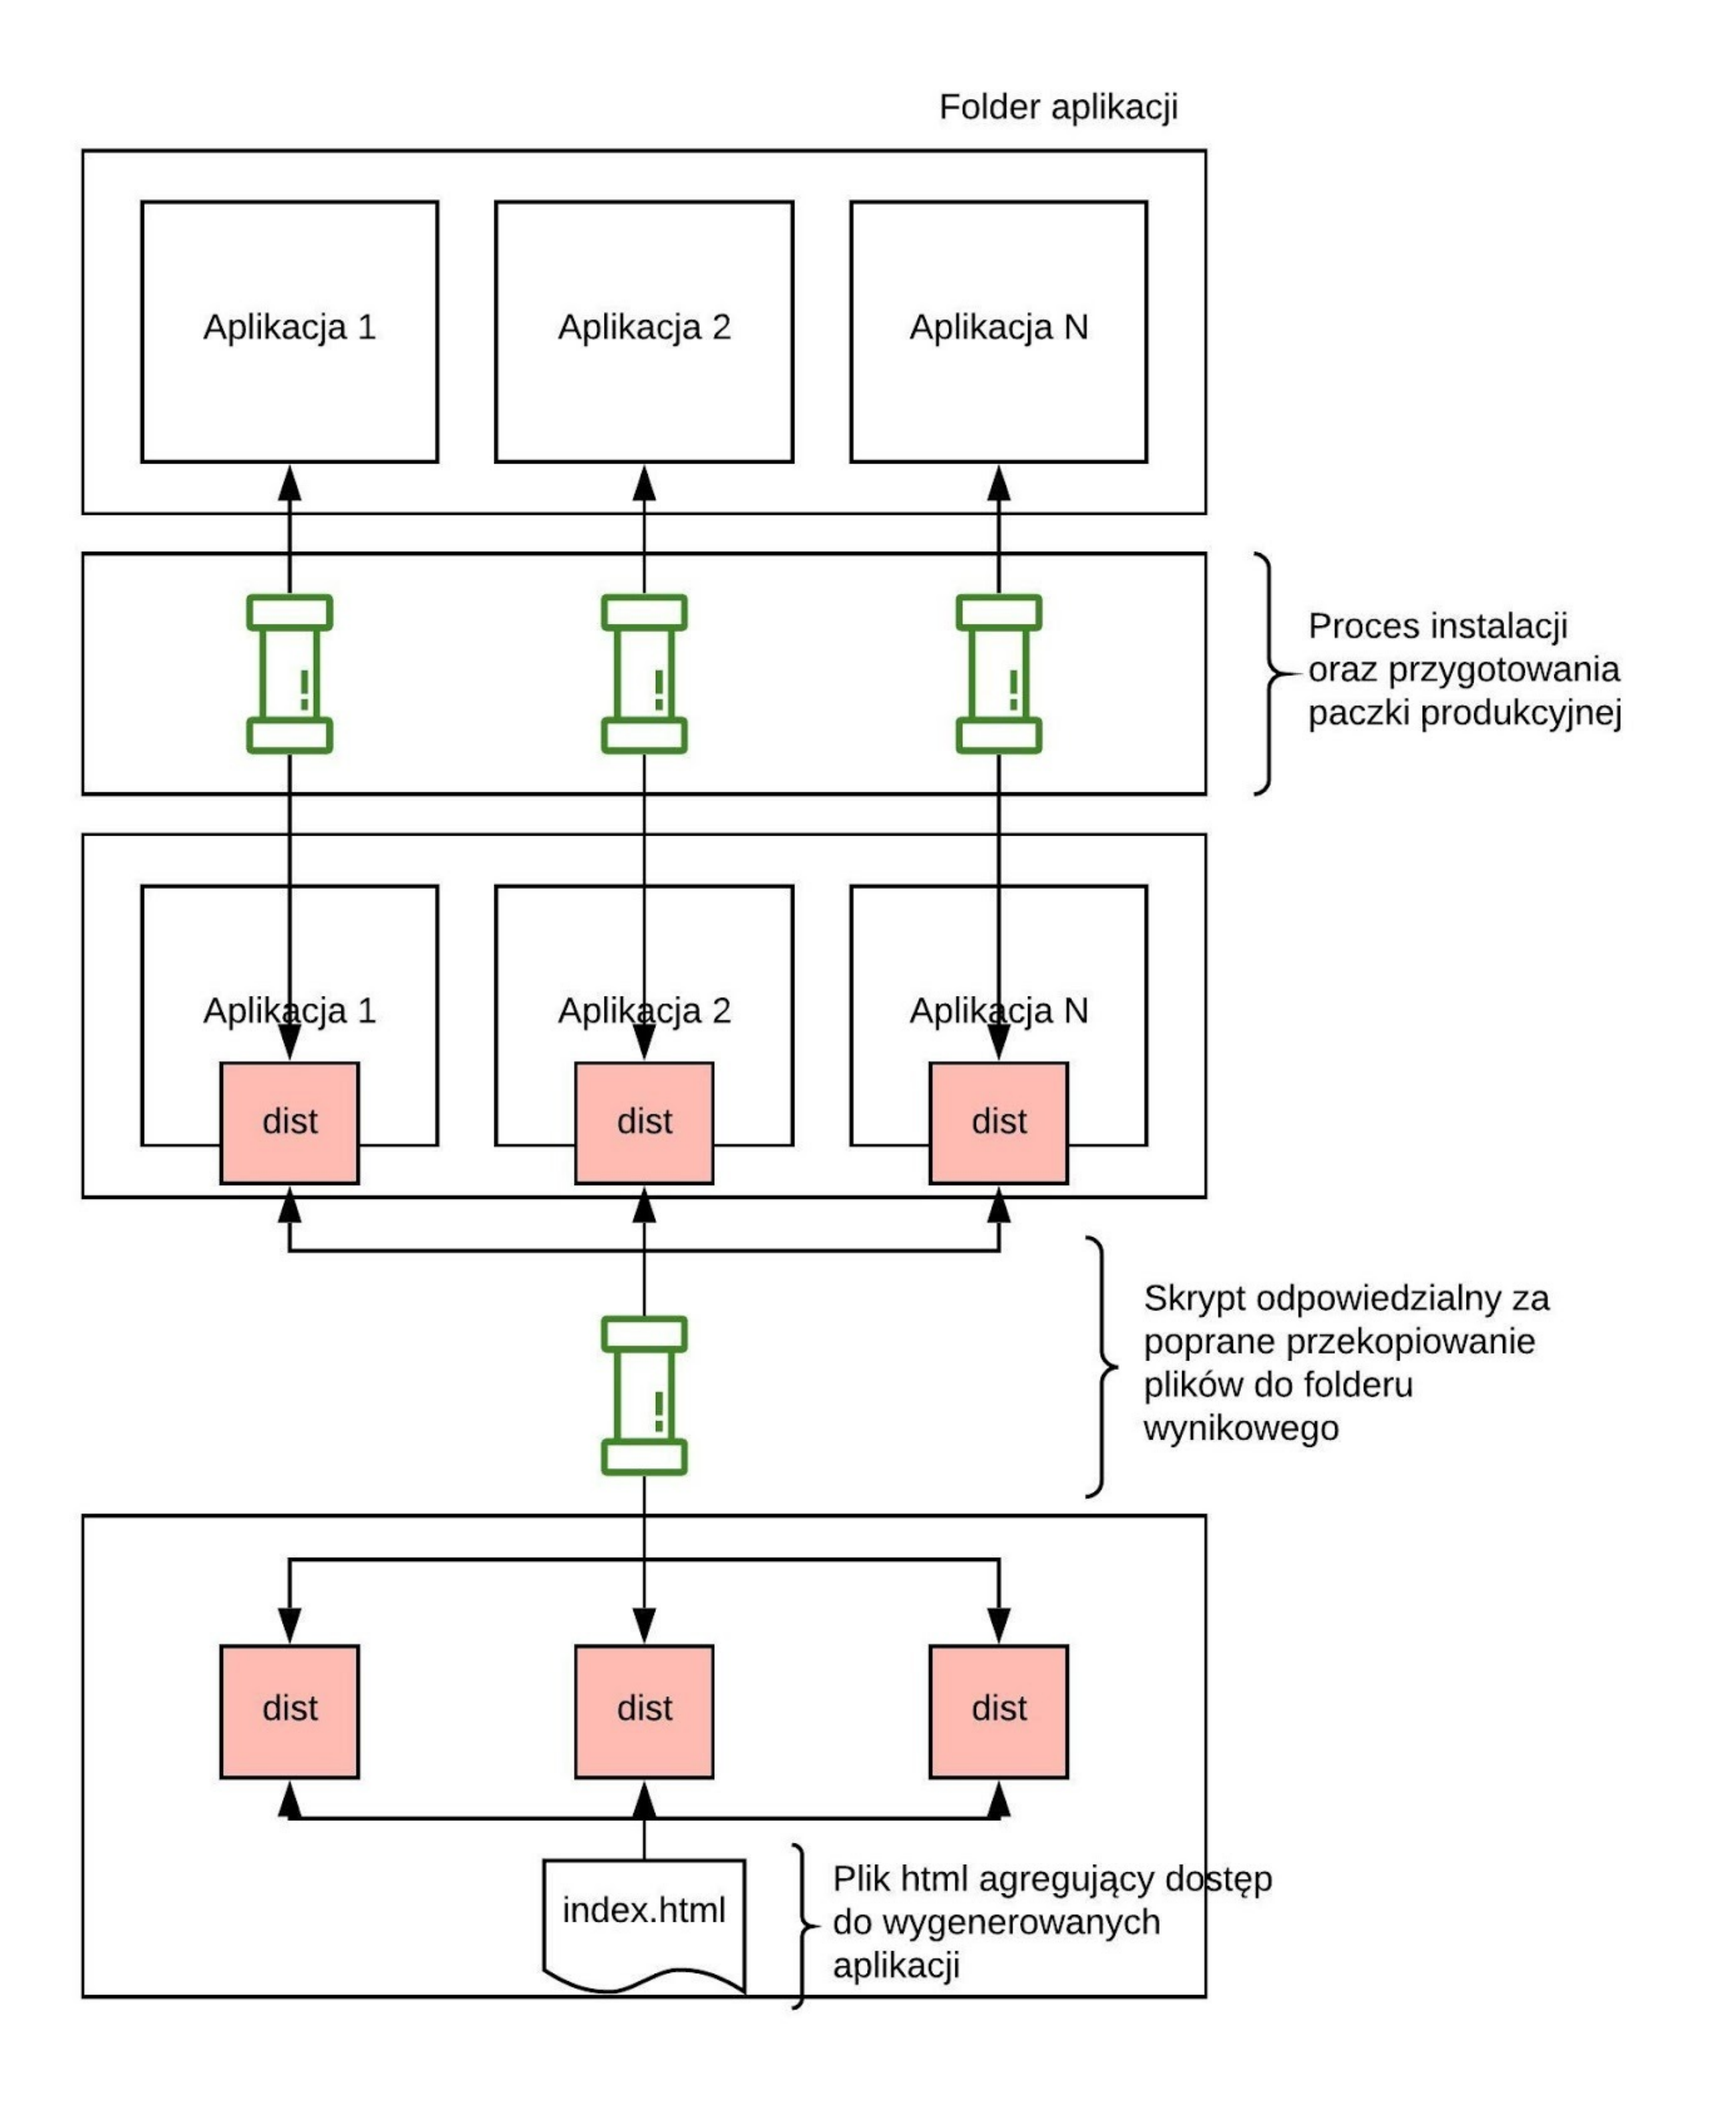
\includegraphics[width=12cm]{rysunek_15.png}
    \caption{Ilustracja procesu przygotowania aplikacji do konteneryzacji}
    \label{fig:rysunek_15}
\end{figure}

\begin{figure}[!ht]
    \centering
    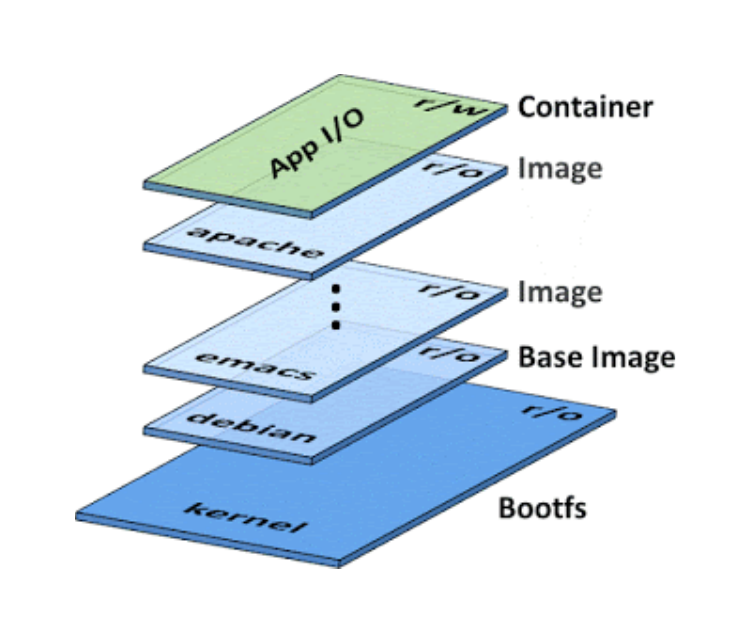
\includegraphics[width=12cm]{rysunek_16.png}
    \caption{Ilustracja przedstawiająca warstwy składające się na  przykładowy obraz dockera}
    \label{fig:rysunek_16}
\end{figure}

\begin{figure}[!ht]
    \centering
    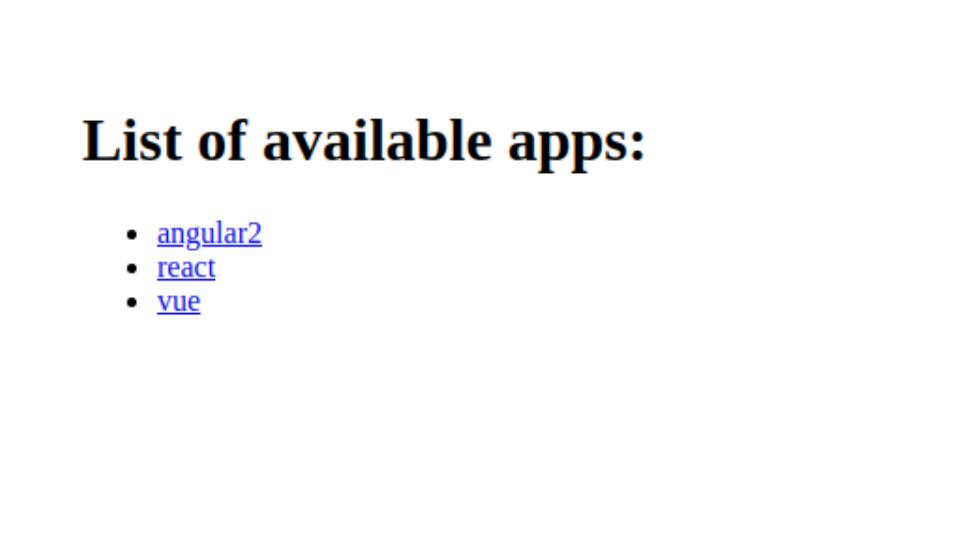
\includegraphics[width=12cm]{rysunek_17.png}
    \caption{Grafika przedstawiająca plik index.html wraz z dostępnymi aplikacjami do badania}
    \label{fig:rysunek_17}
\end{figure}

\begin{figure}[!ht]
    \centering
    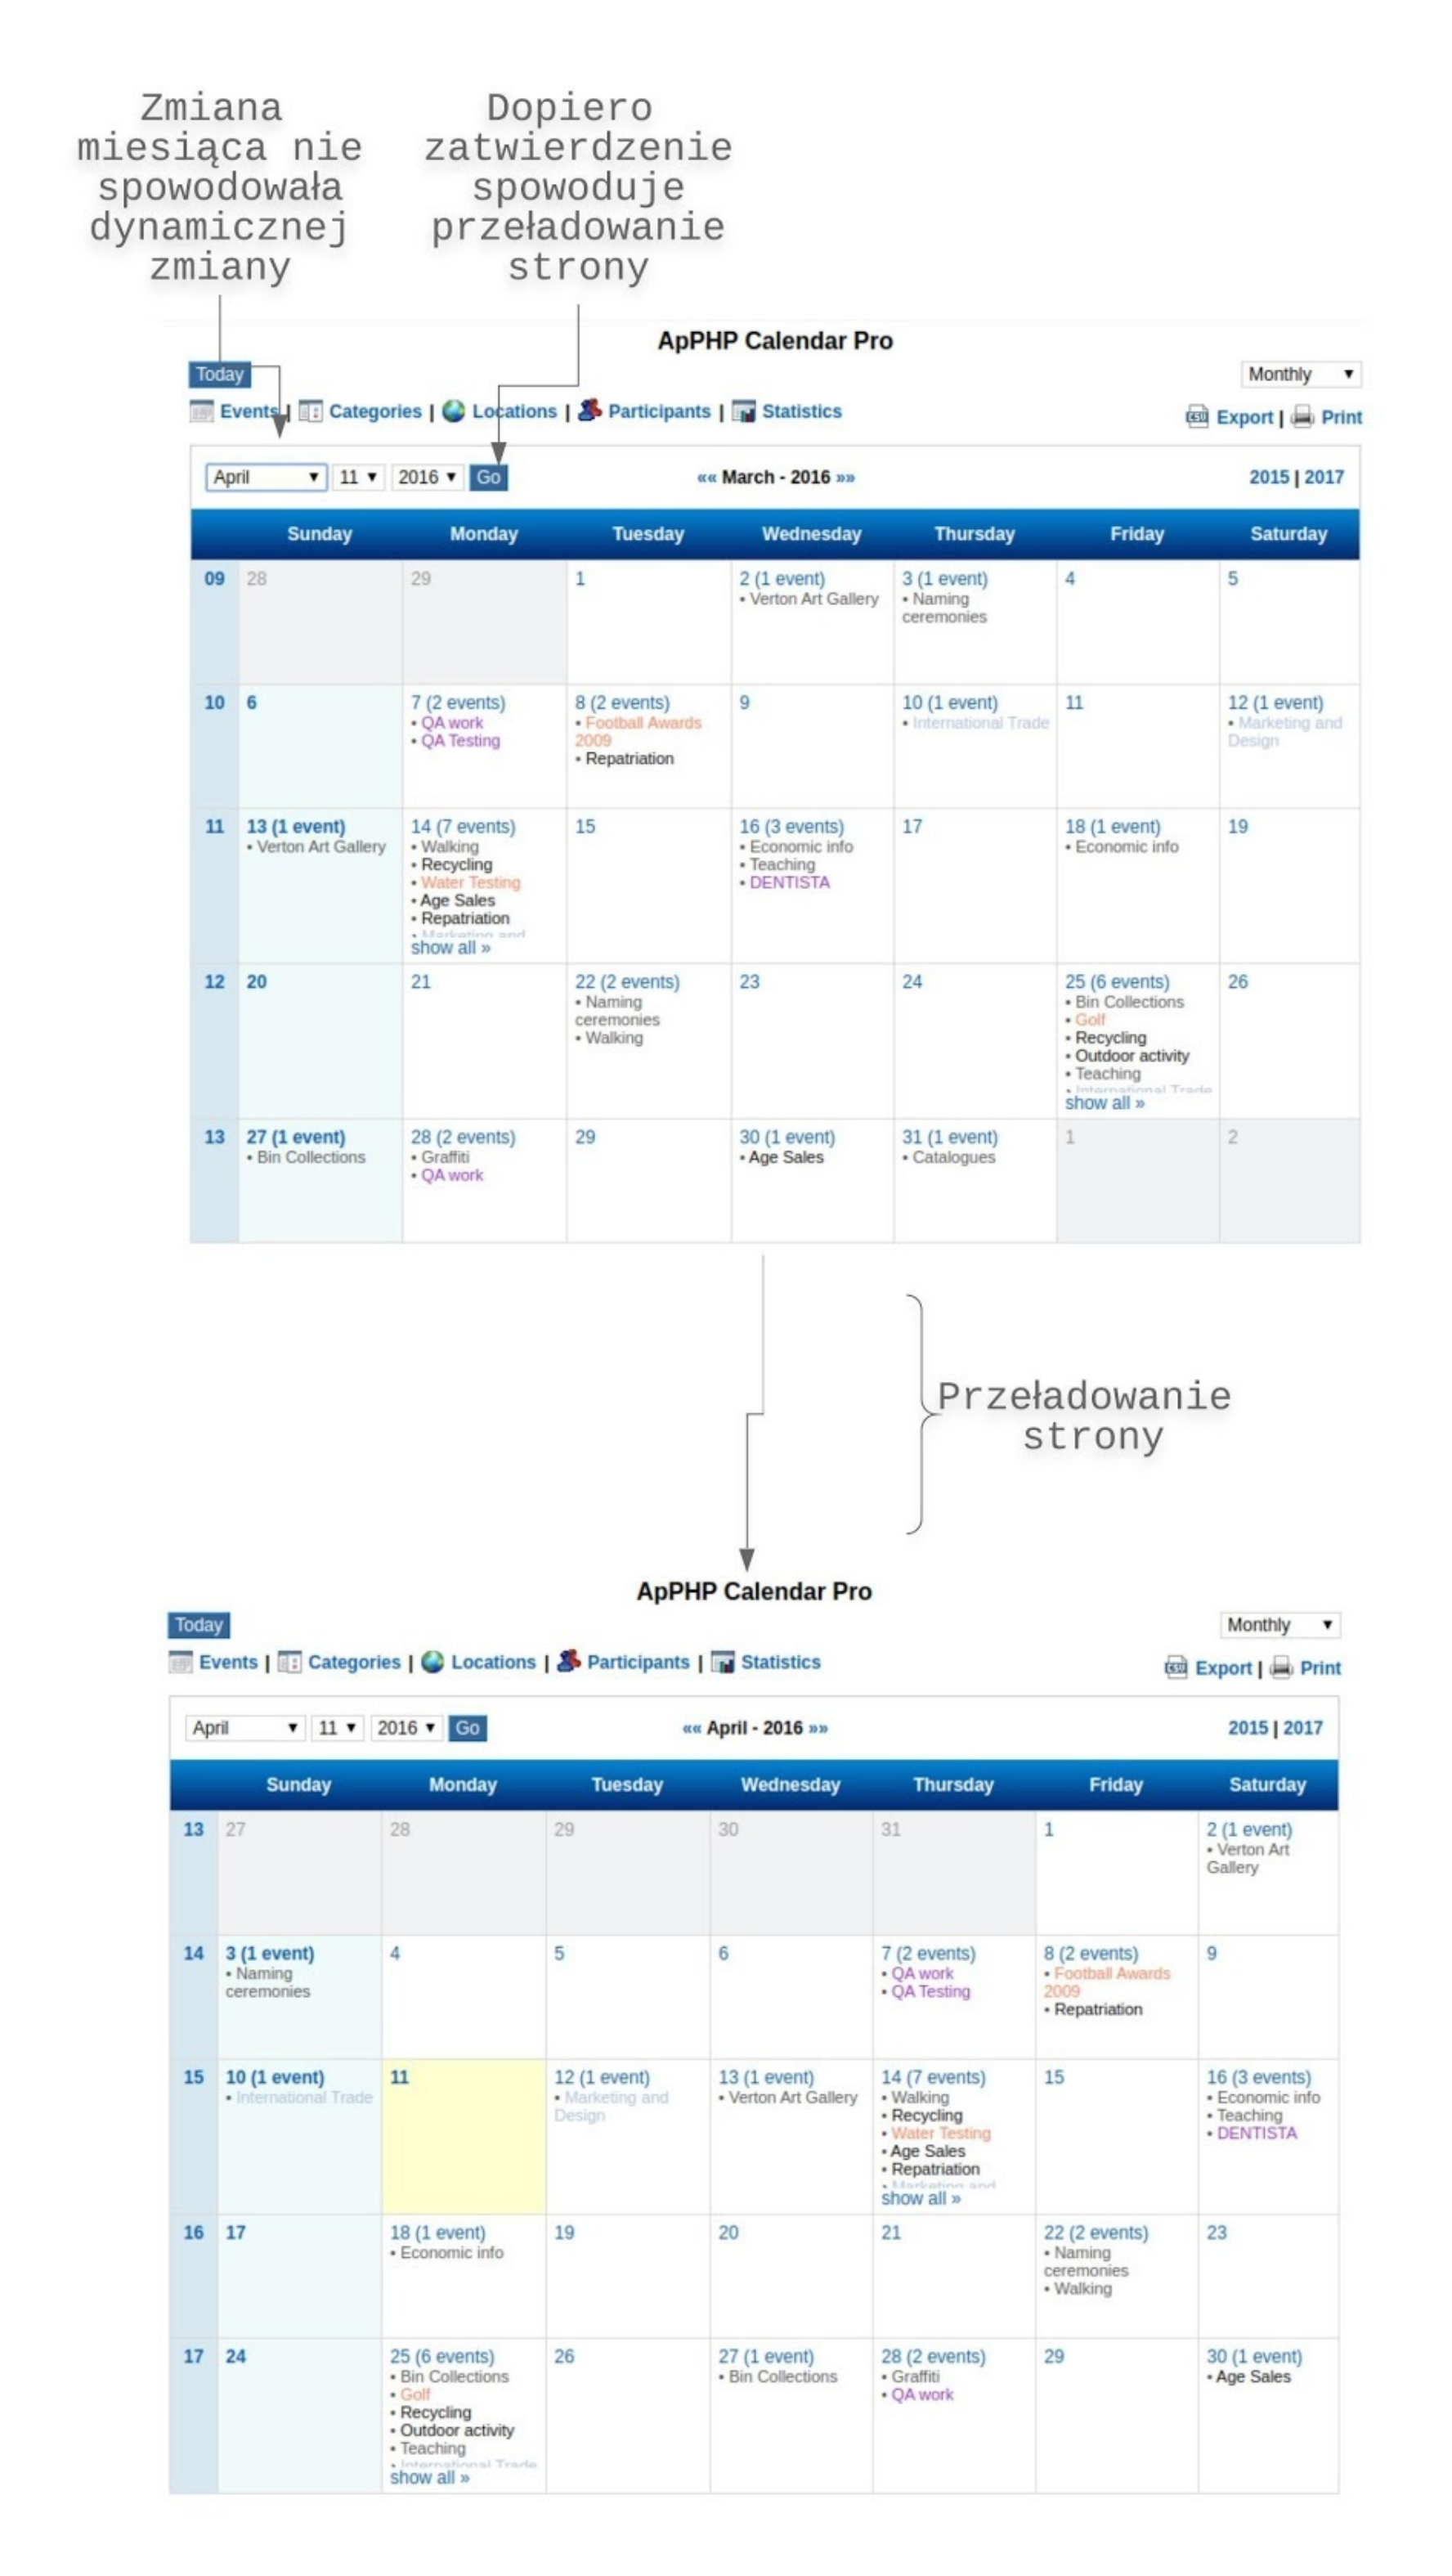
\includegraphics[width=12cm]{rysunek_18.png}
    \caption{Ilustracja mechanizmu działania strony statycznej na przykładzie aplikacji kalendarza przy użyciu języka PHP}
    \label{fig:rysunek_18}
\end{figure}

\begin{figure}[!ht]
    \centering
    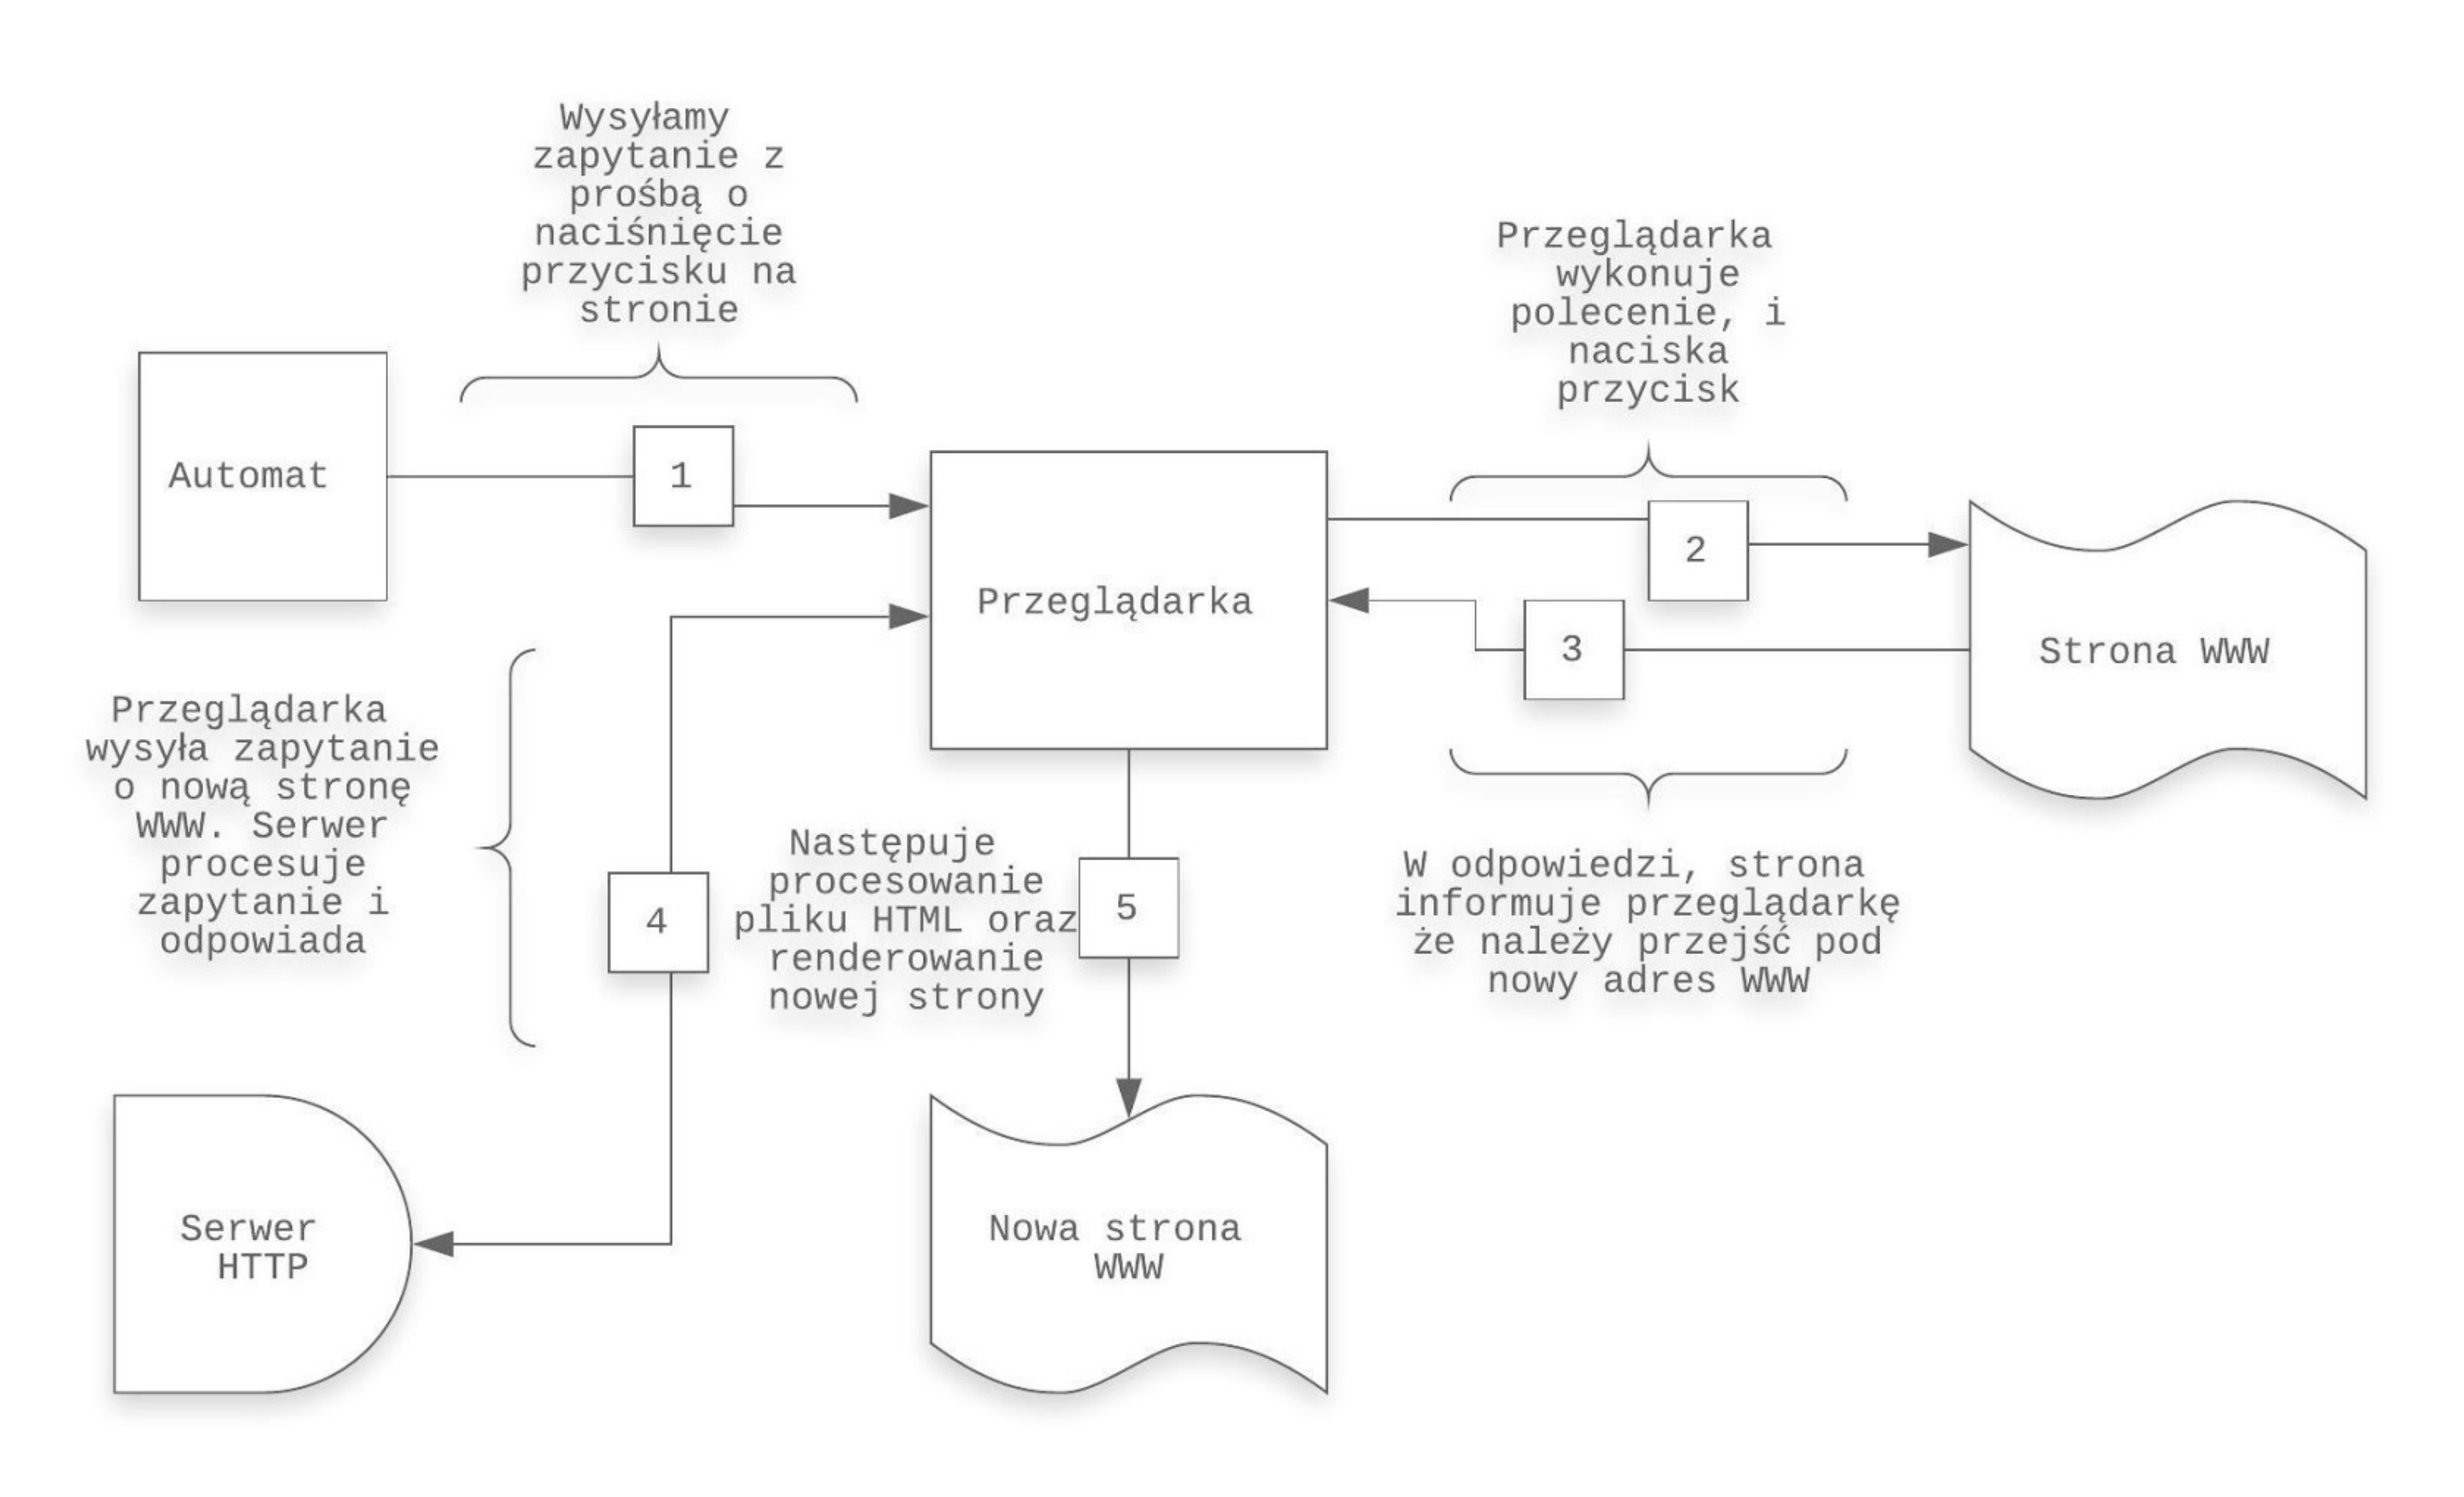
\includegraphics[width=12cm]{rysunek_19.png}
    \caption{Grafika przedstawiająca proces przeładowania strony statycznej}
    \label{fig:rysunek_19}
\end{figure}

\begin{figure}[!ht]
    \centering
    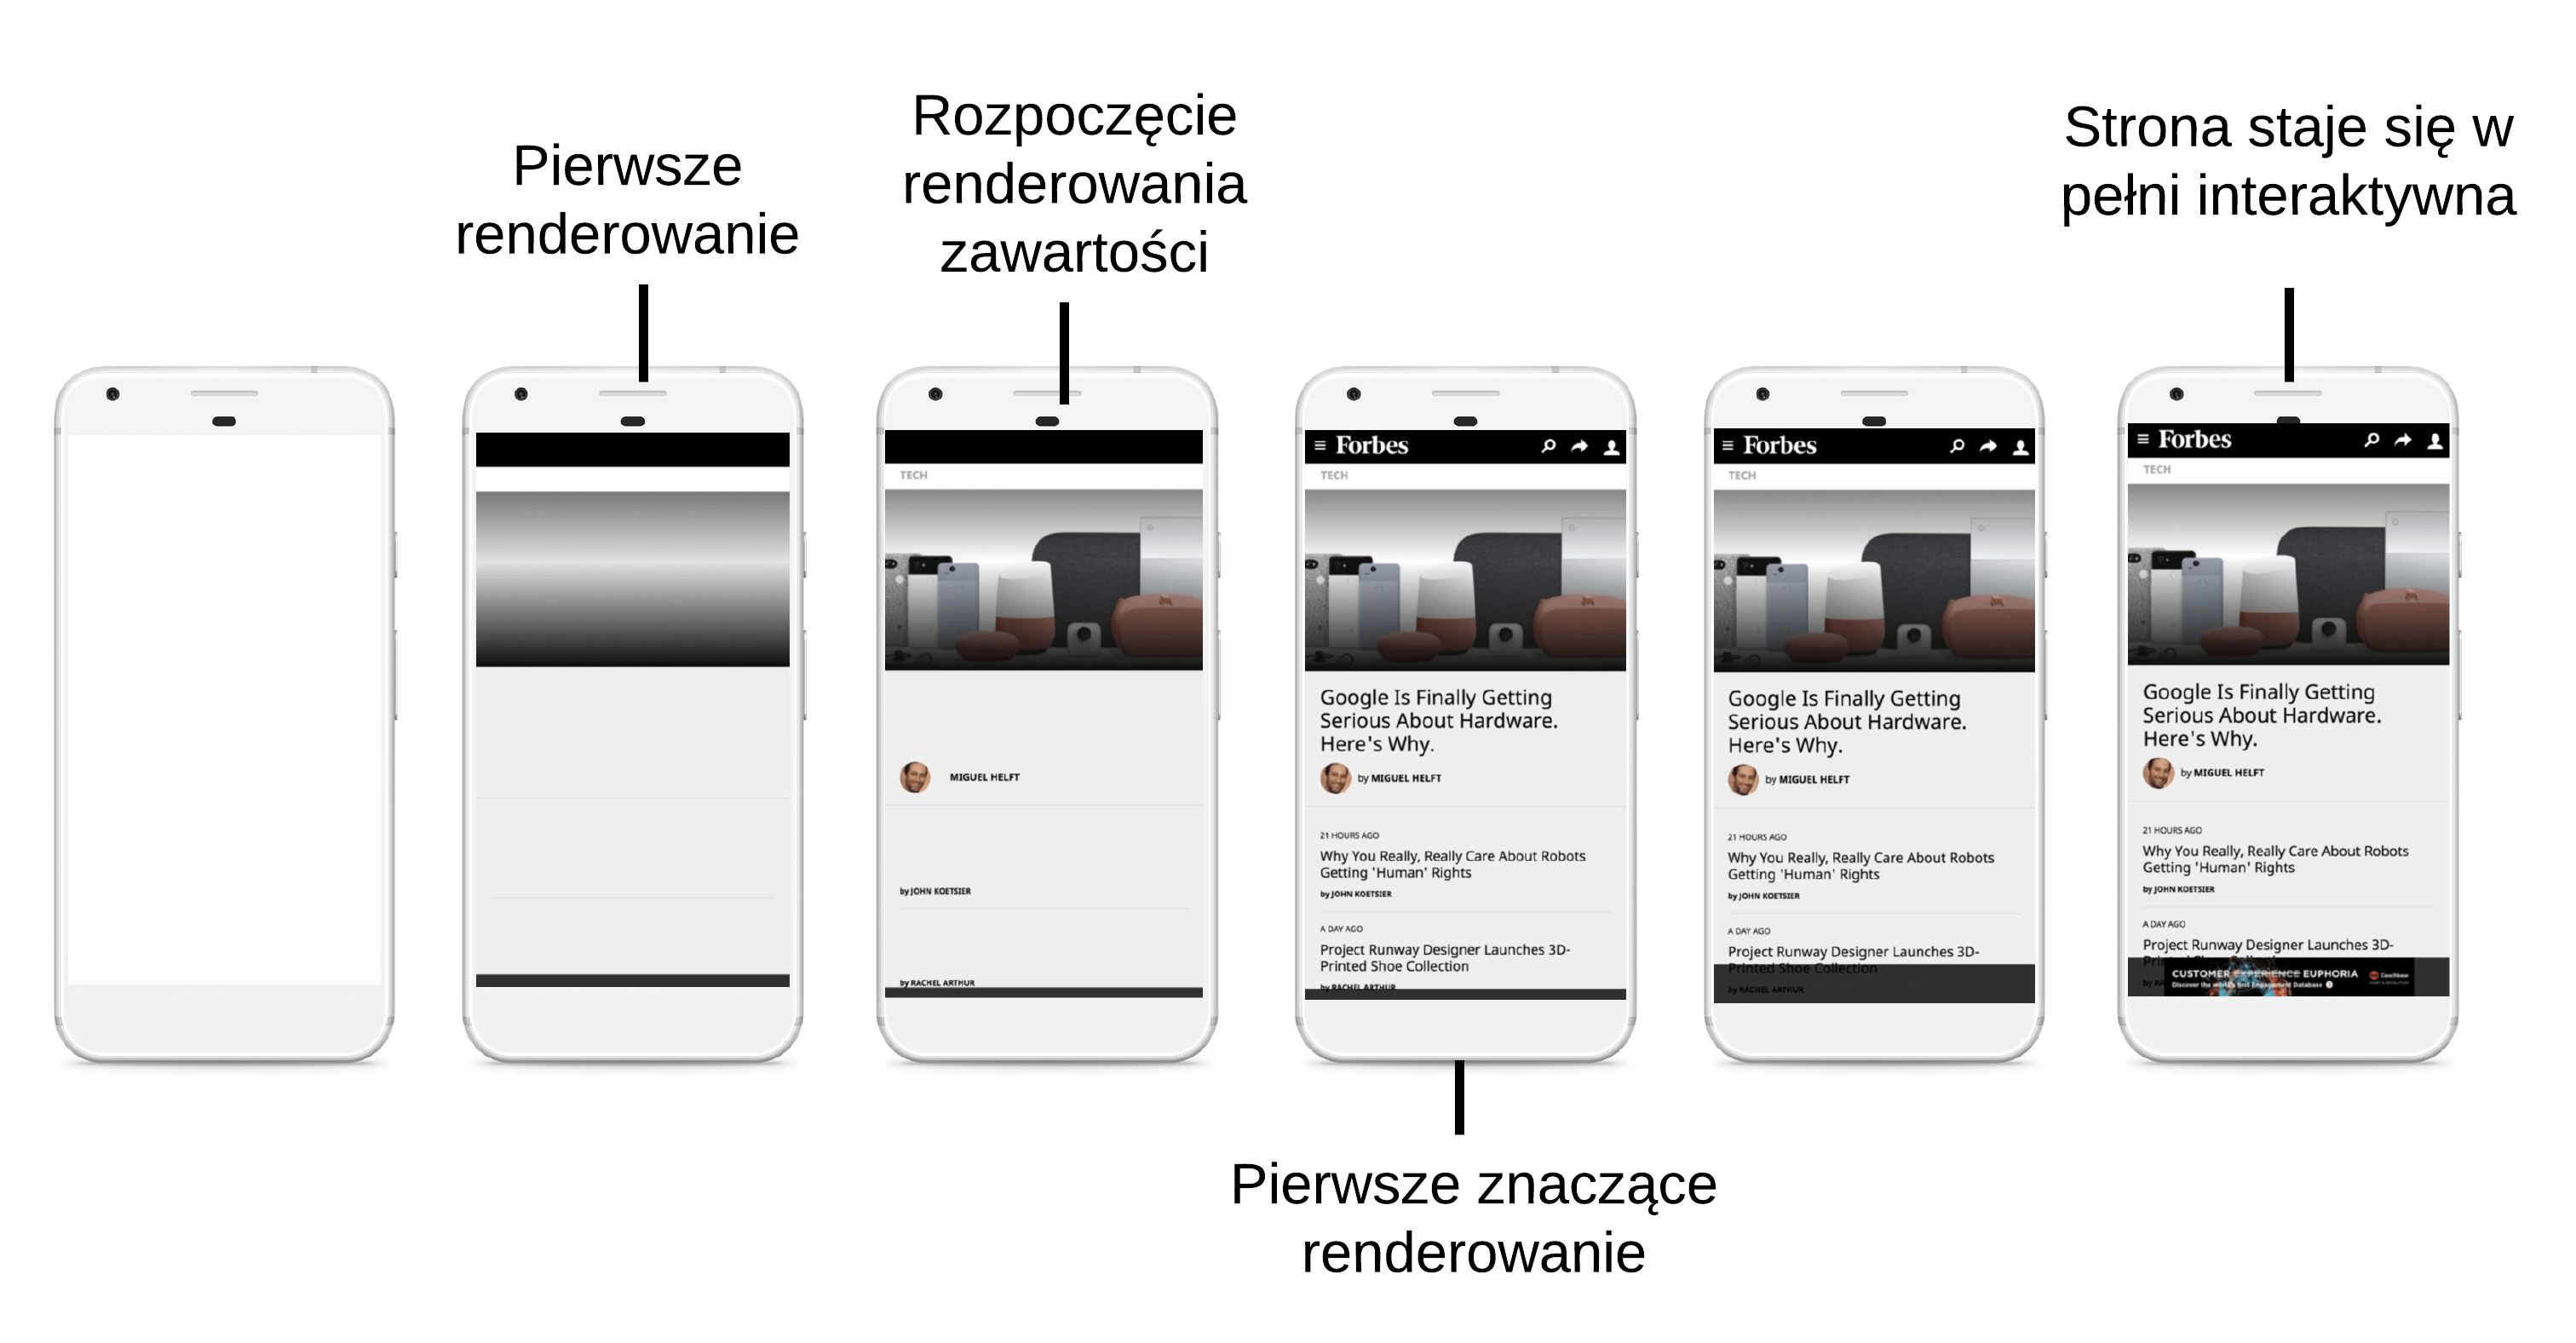
\includegraphics[width=12cm]{rysunek_20.png}
    \caption{Ilustracja procesu ładowania aplikacji oraz zdarzenia rejestrowane przez przeglądarkę}
    \label{fig:rysunek_20}
\end{figure}

\begin{figure}[!ht]
    \centering
    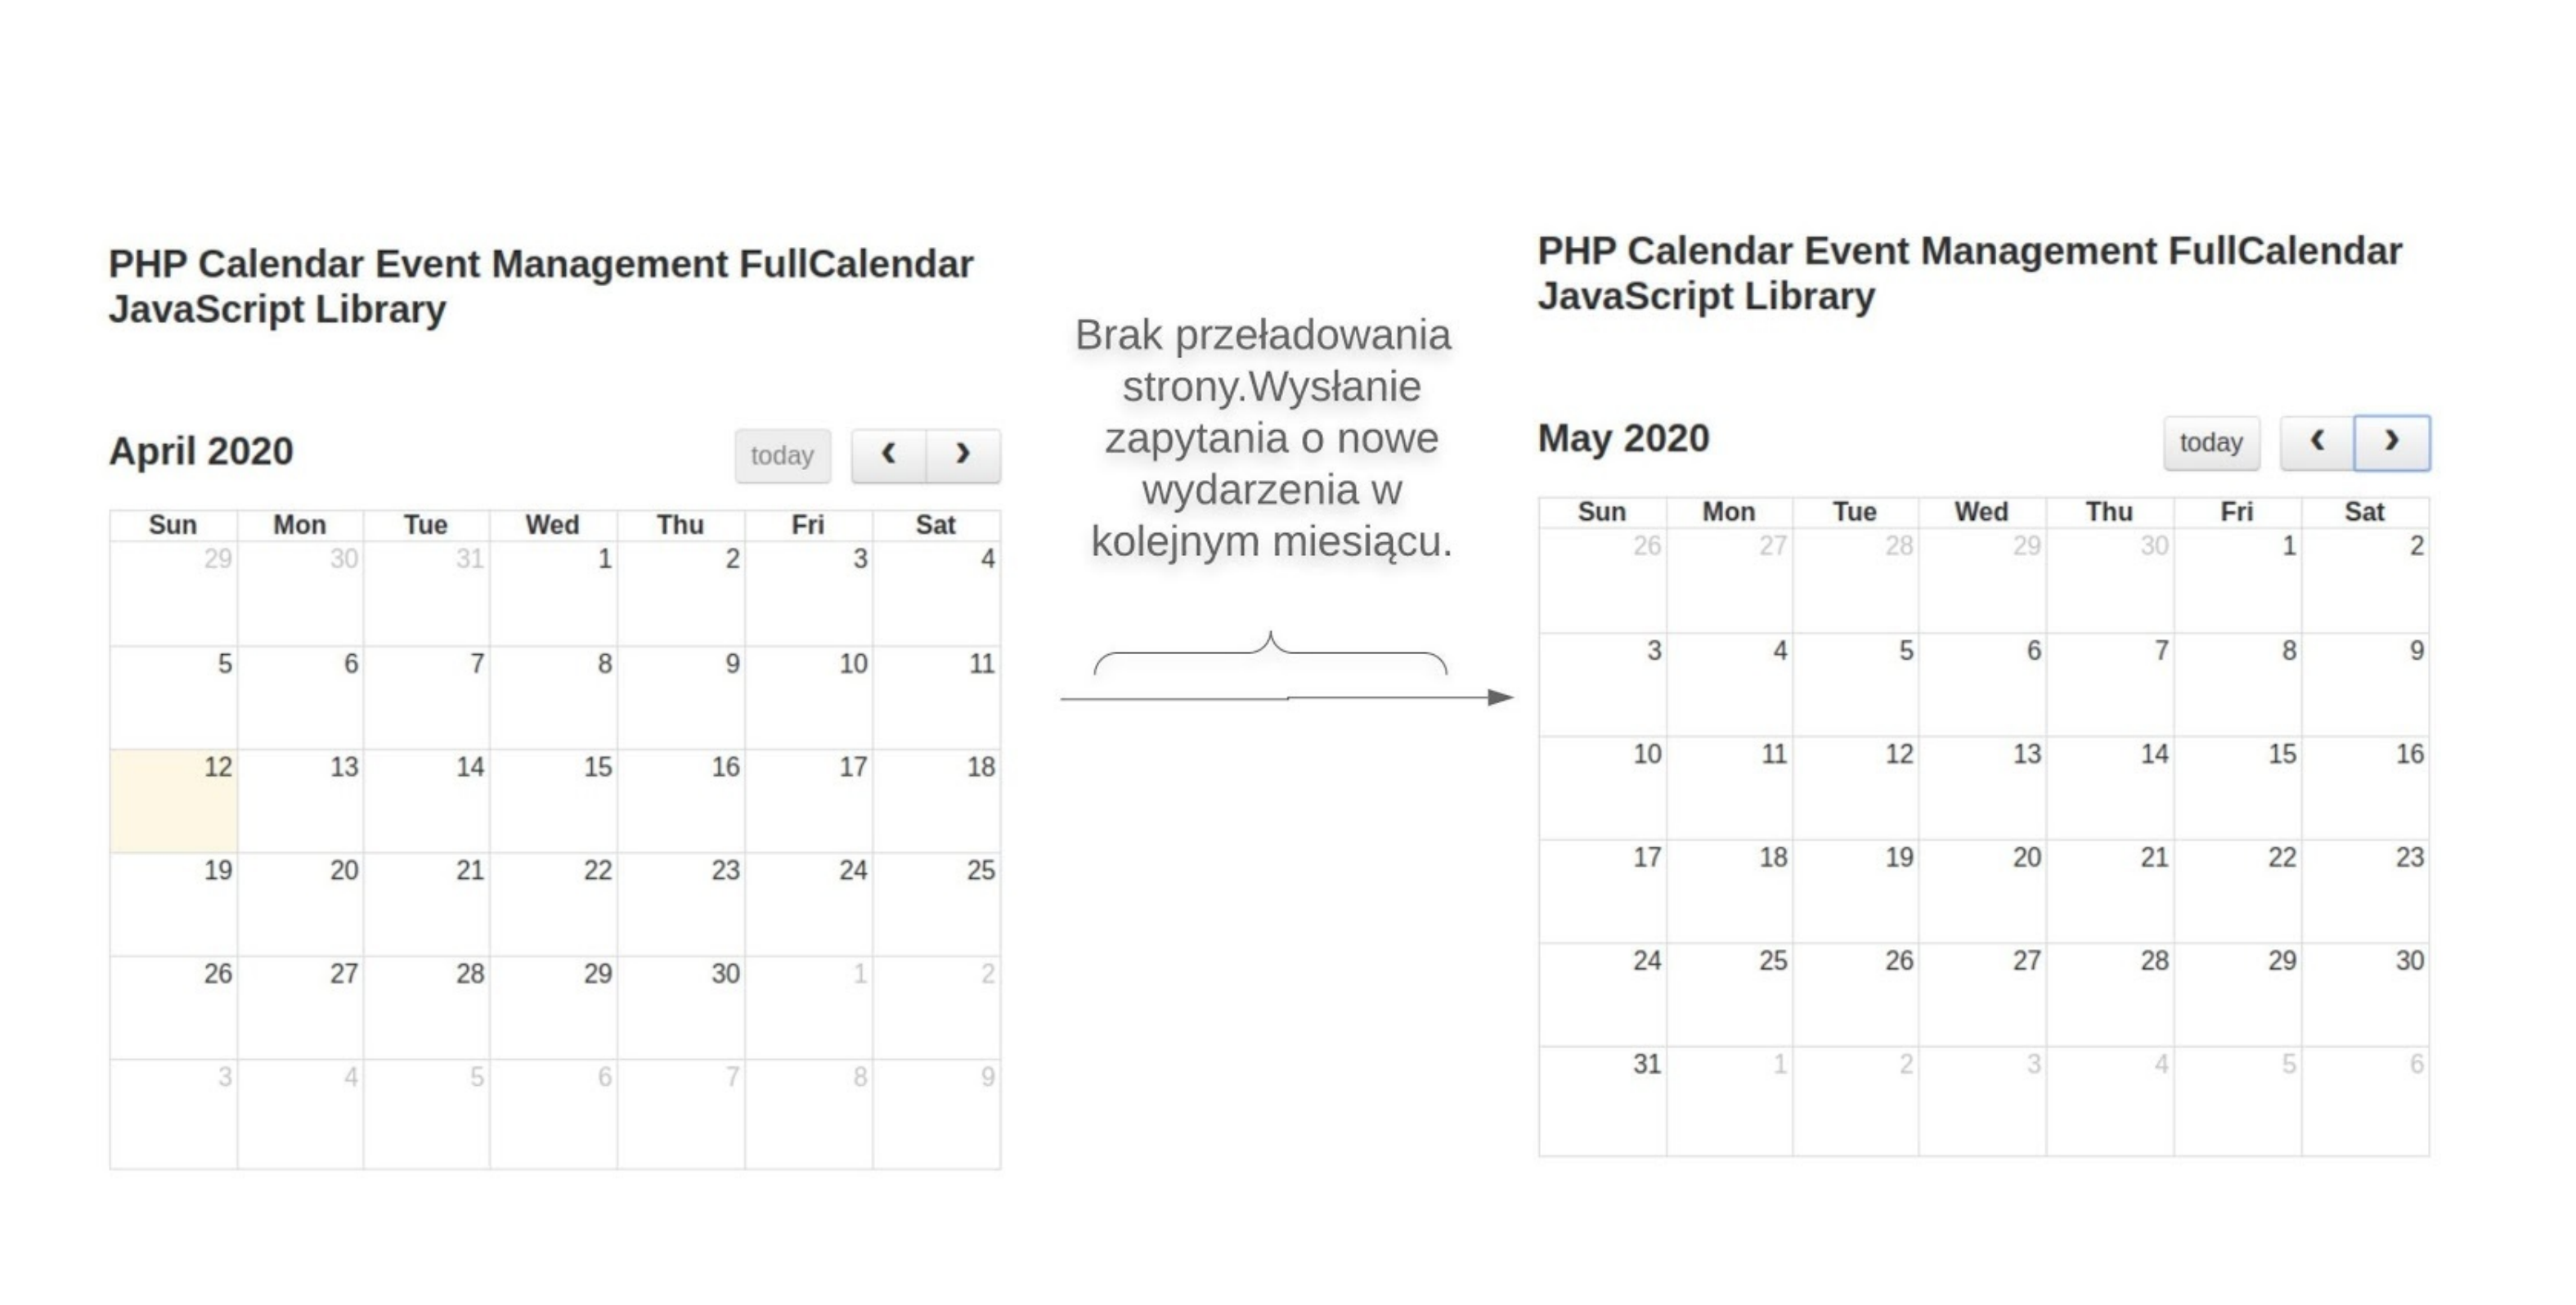
\includegraphics[width=12cm]{rysunek_21.png}
    \caption{Ilustracja mechanizmu zmiany daty w przypadku aplikacji dynamicznej}
    \label{fig:rysunek_21}
\end{figure}

\begin{figure}[!ht]
    \centering
    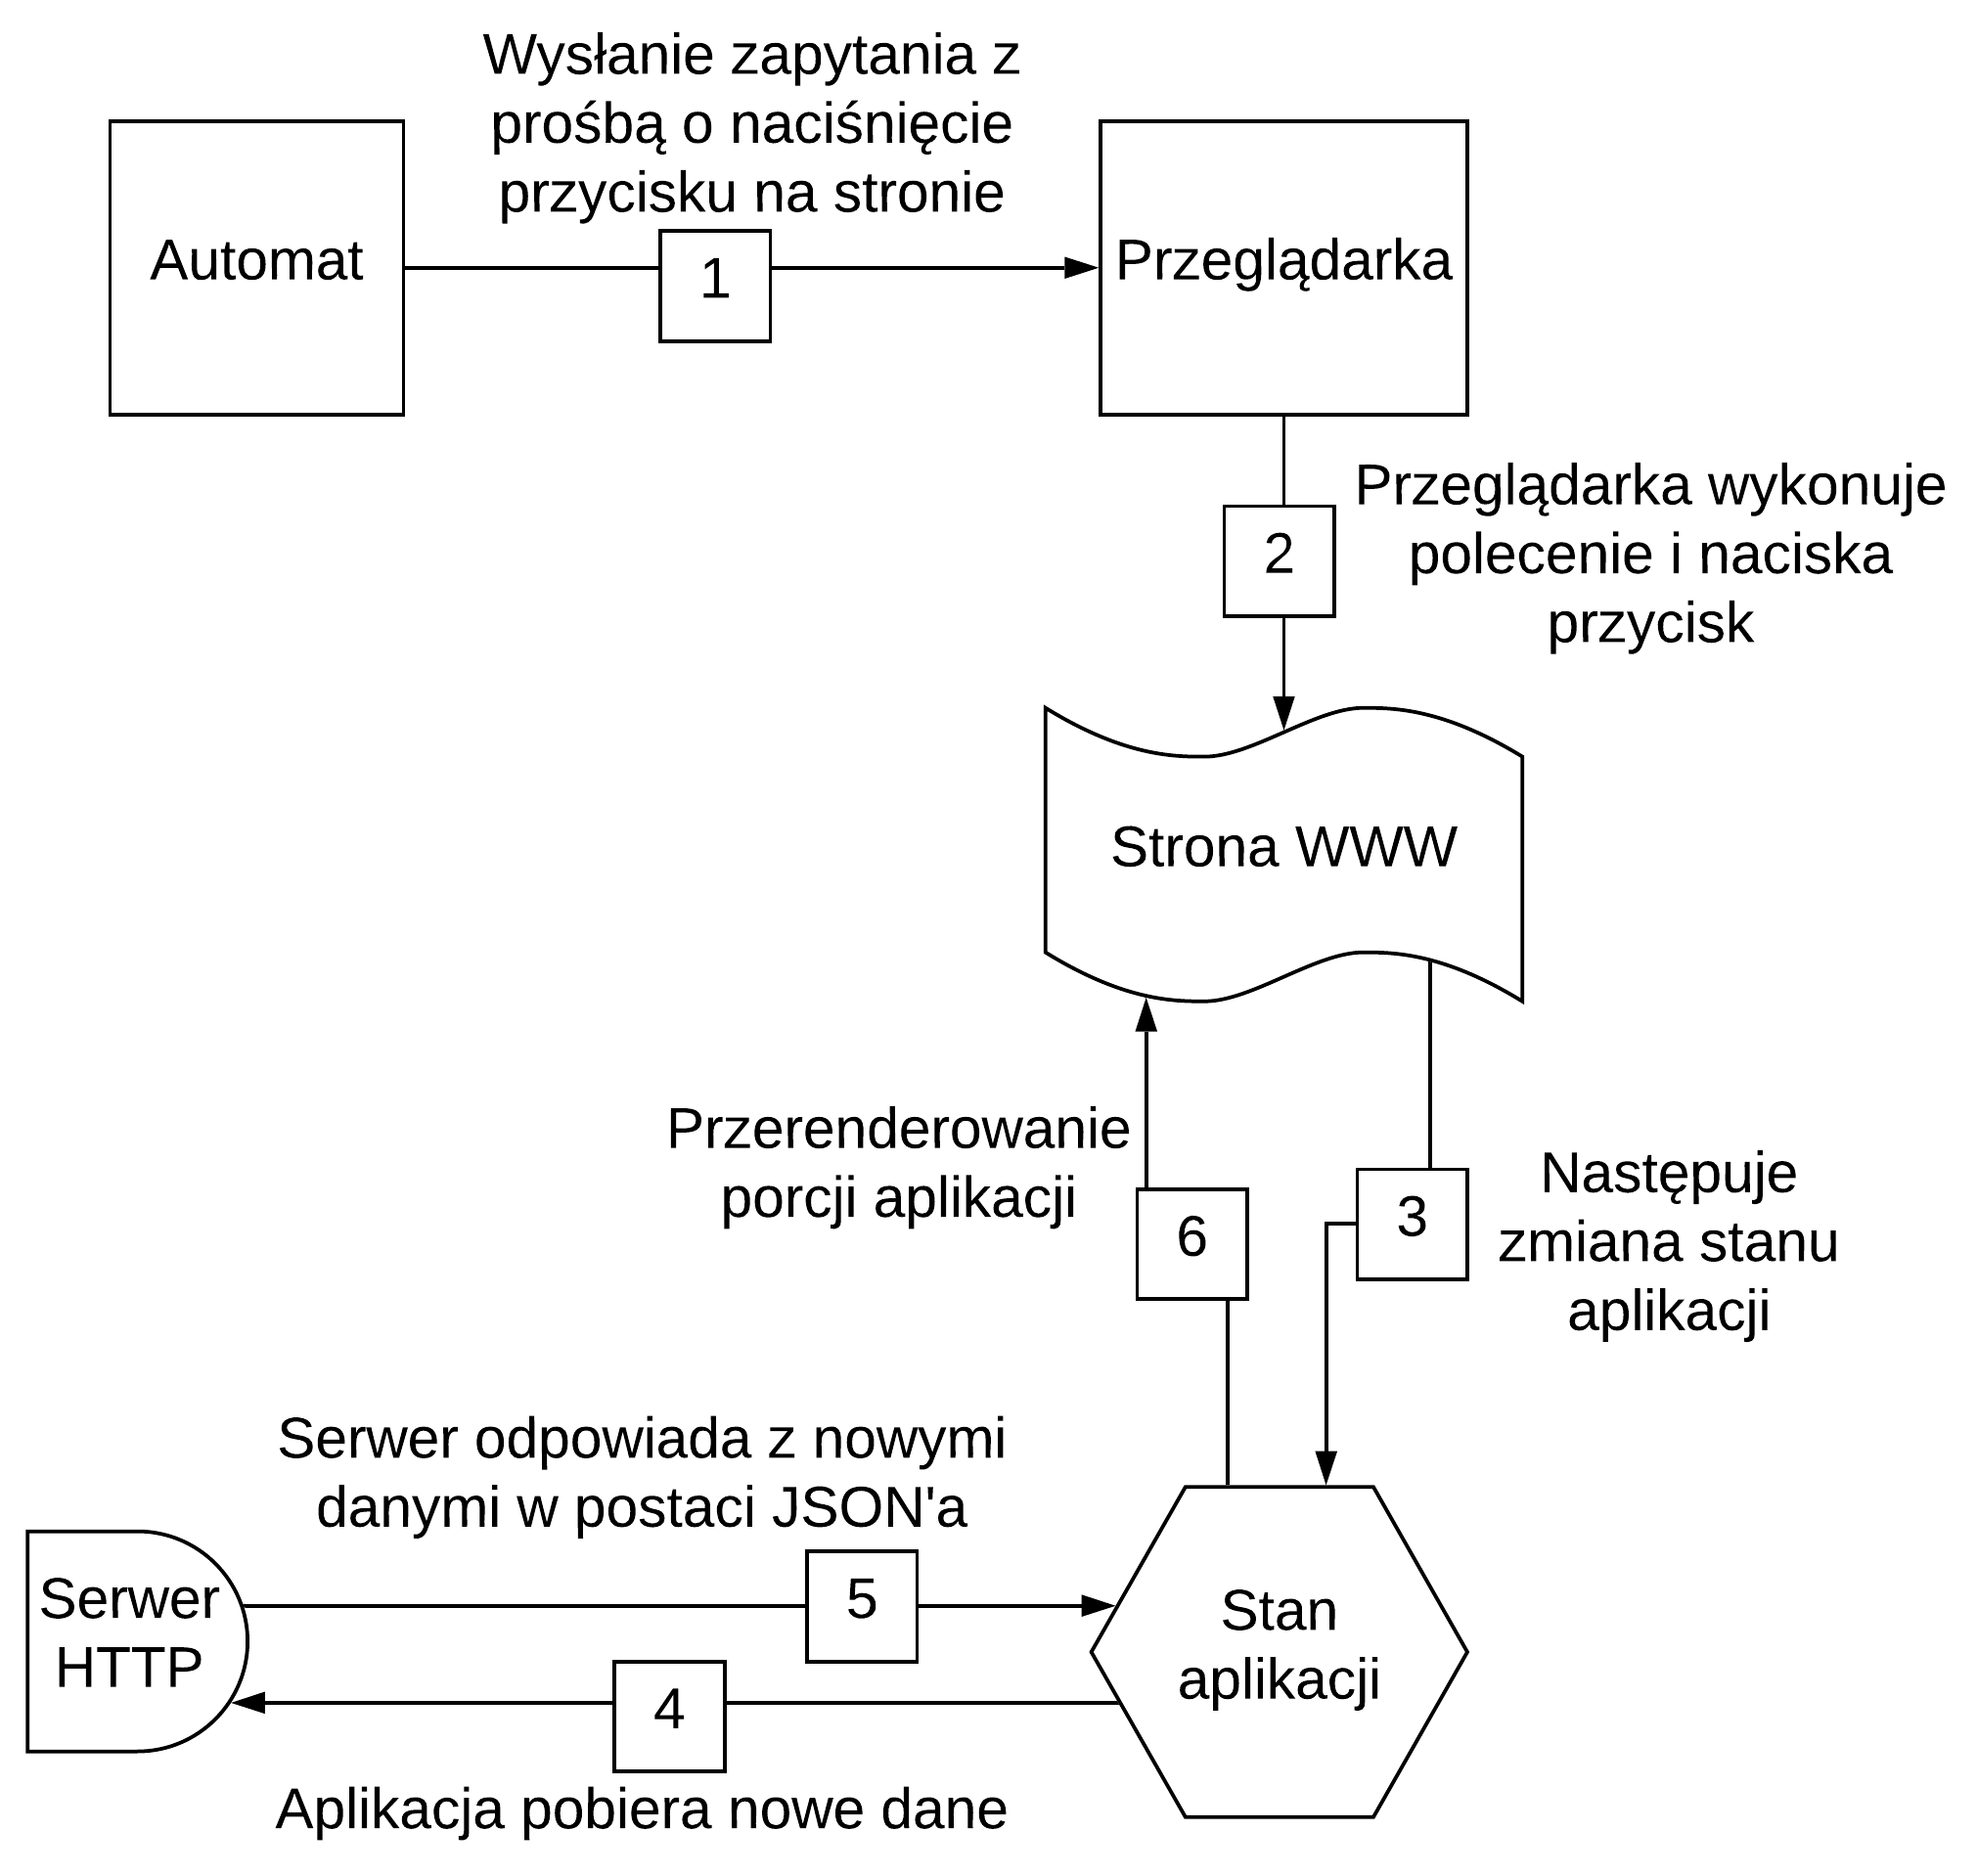
\includegraphics[width=12cm]{rysunek_22.png}
    \caption{Ilustracja przedstawiająca proces zmiany treści strony w przypadku aplikacji dynamicznej}
    \label{fig:rysunek_22}
\end{figure}

\begin{figure}[!ht]
    \centering
    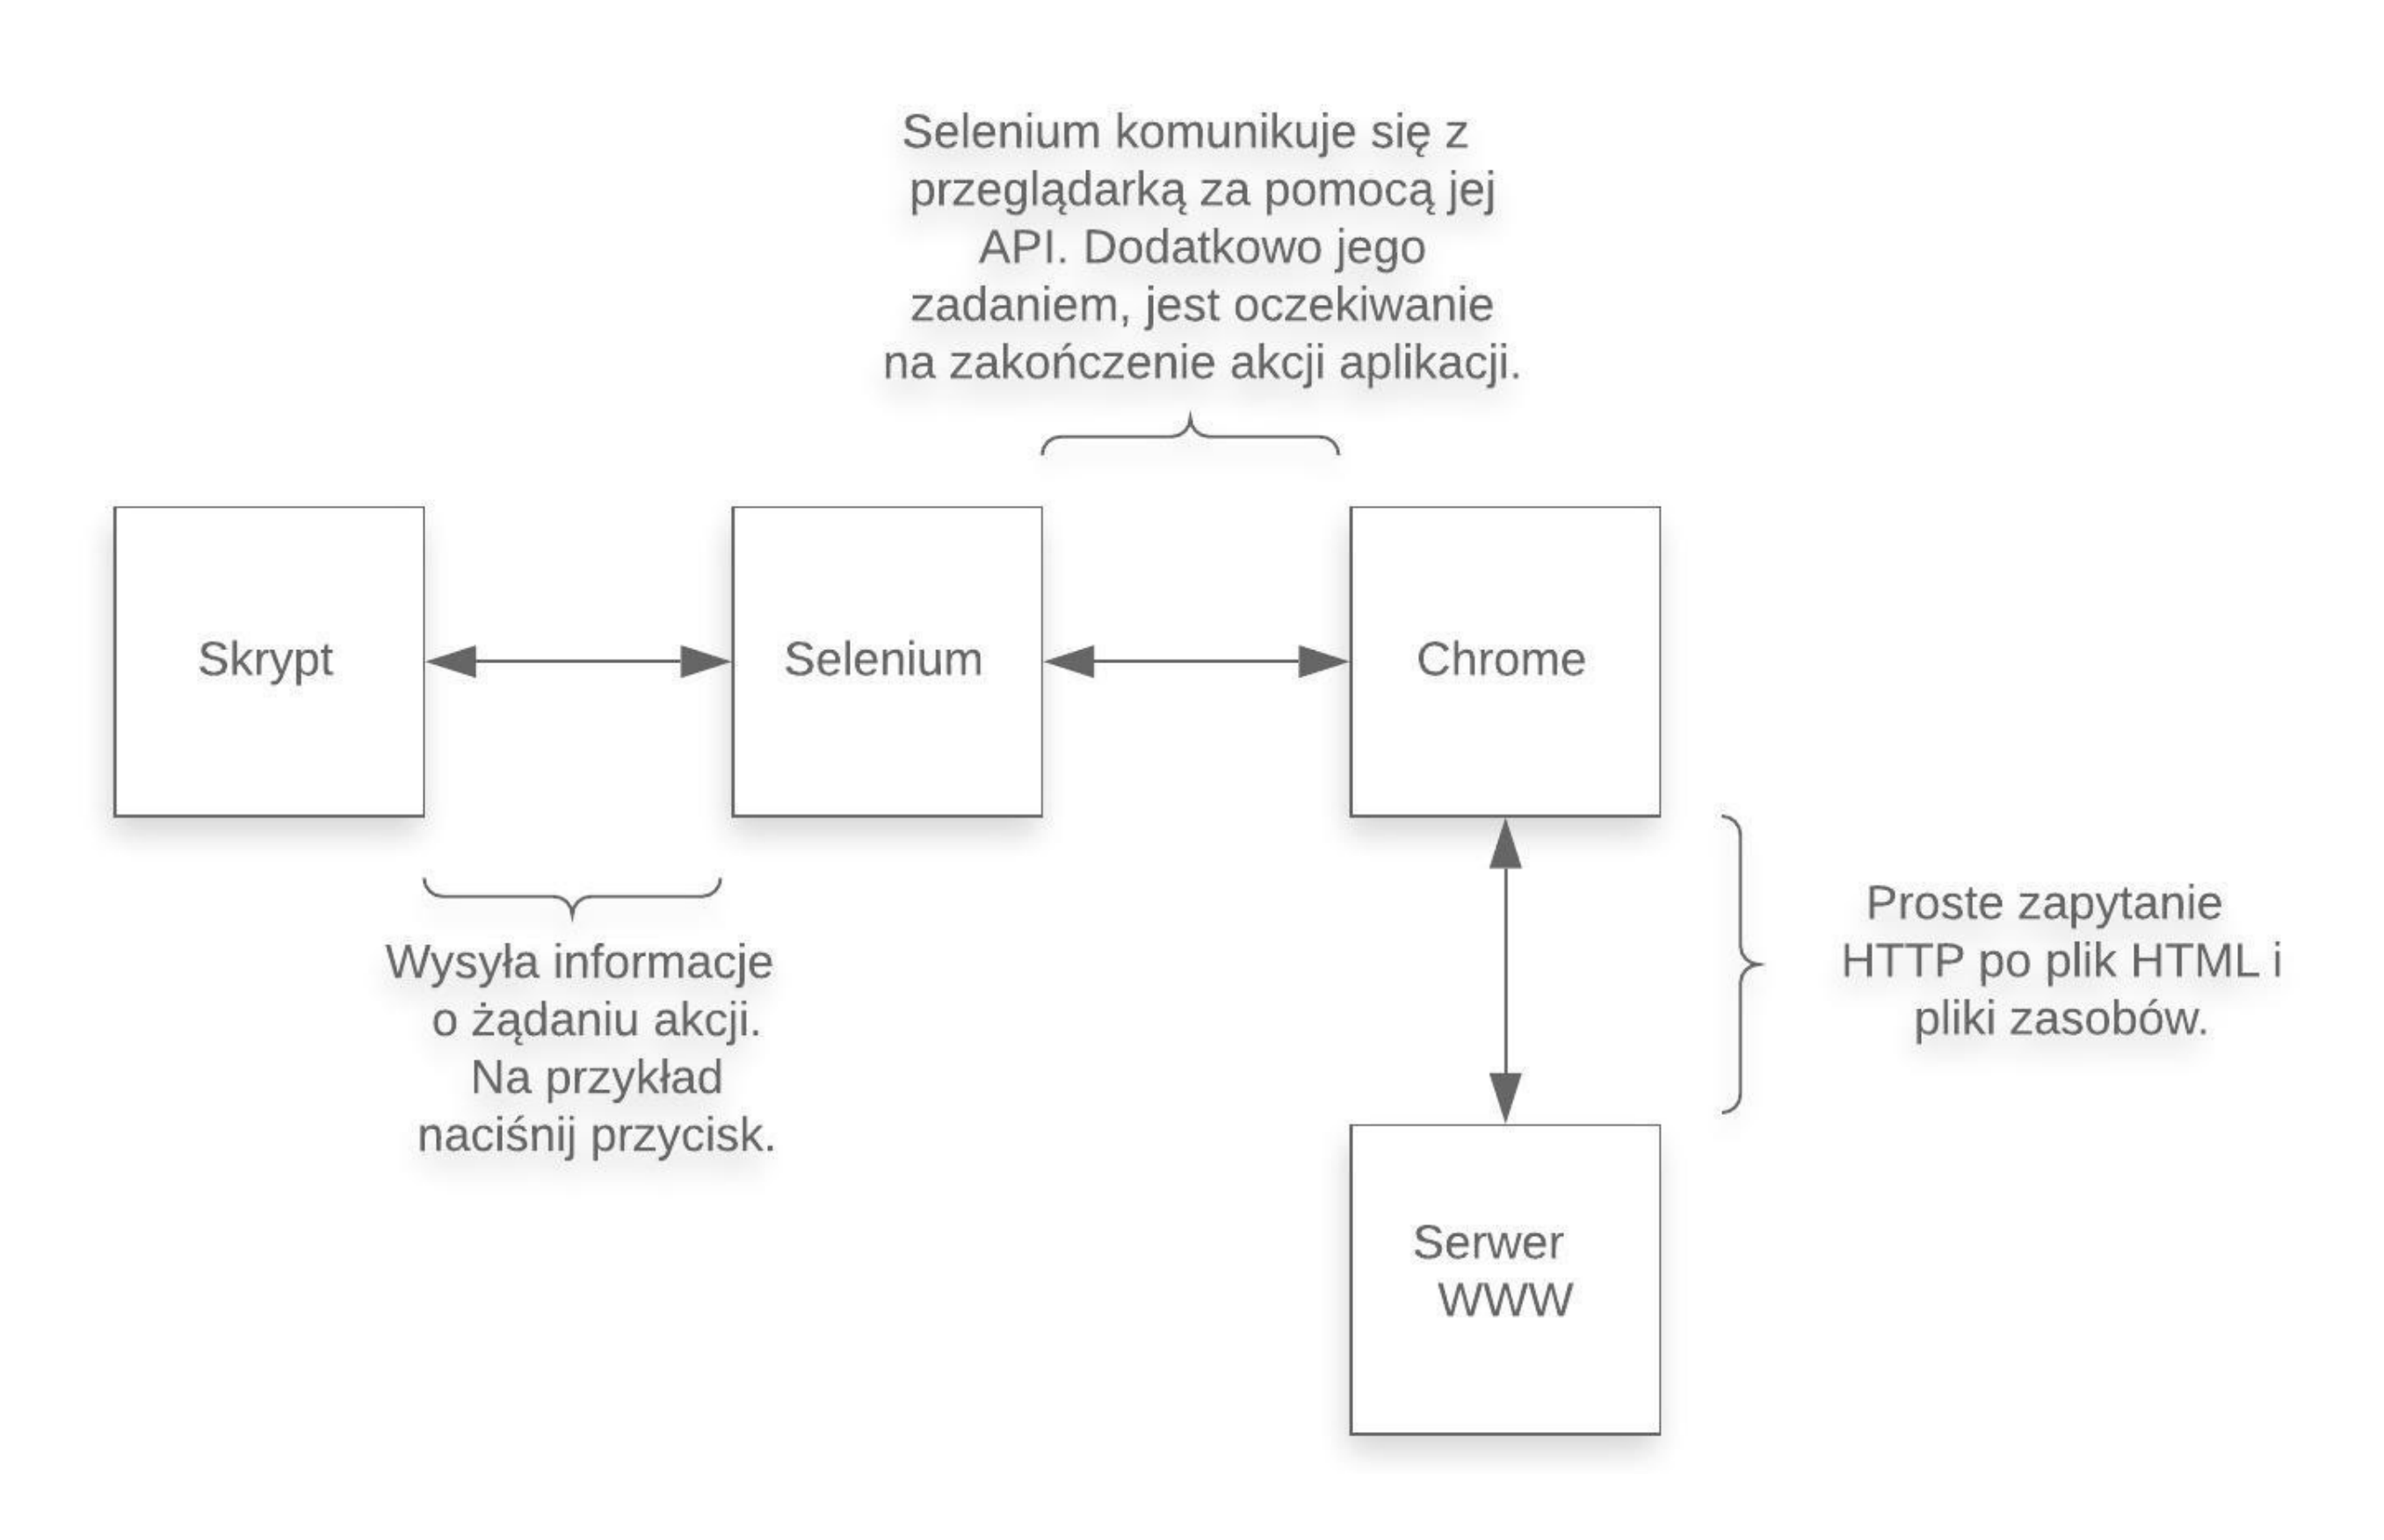
\includegraphics[width=12cm]{rysunek_23.png}
    \caption{Ilustracja procesu współpracy pomiędzy Selenium a przeglądarką}
    \label{fig:rysunek_23}
\end{figure}

\begin{figure}[!ht]
    \centering
    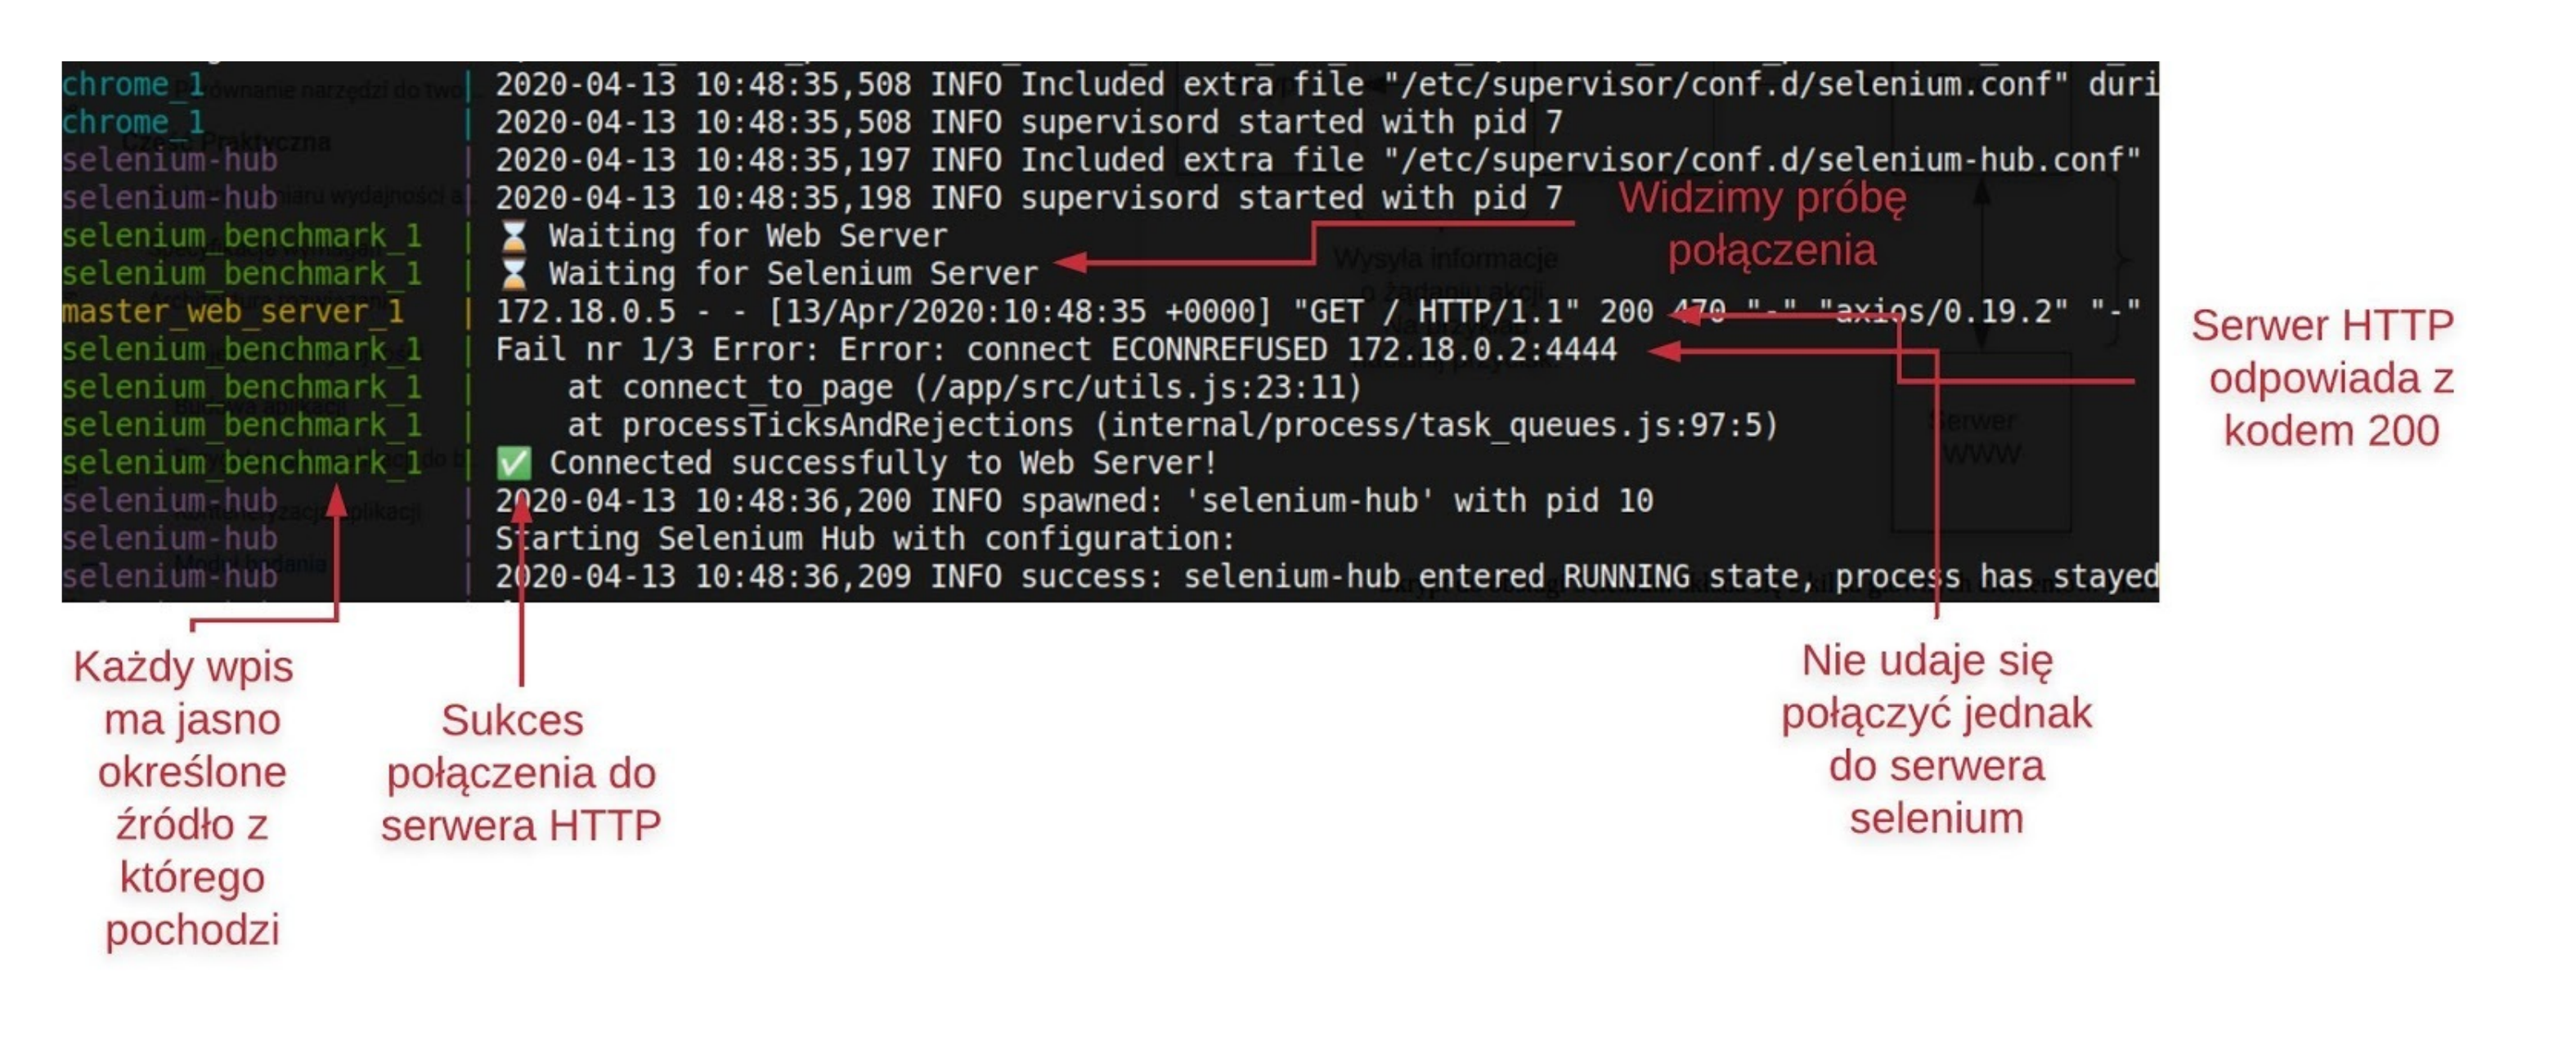
\includegraphics[width=12cm]{rysunek_24.png}
    \caption{Wycinek wpisów skryptu przeprowadzającego badanie w środowisku docker-compose. Ilustruje on inicjalizację skryptu oraz mechanizm uzyskiwania połączenia pomiędzy Skryptem - Przeglądarką - Selenium}
    \label{fig:rysunek_24}
\end{figure}

\begin{figure}[!ht]
    \centering
    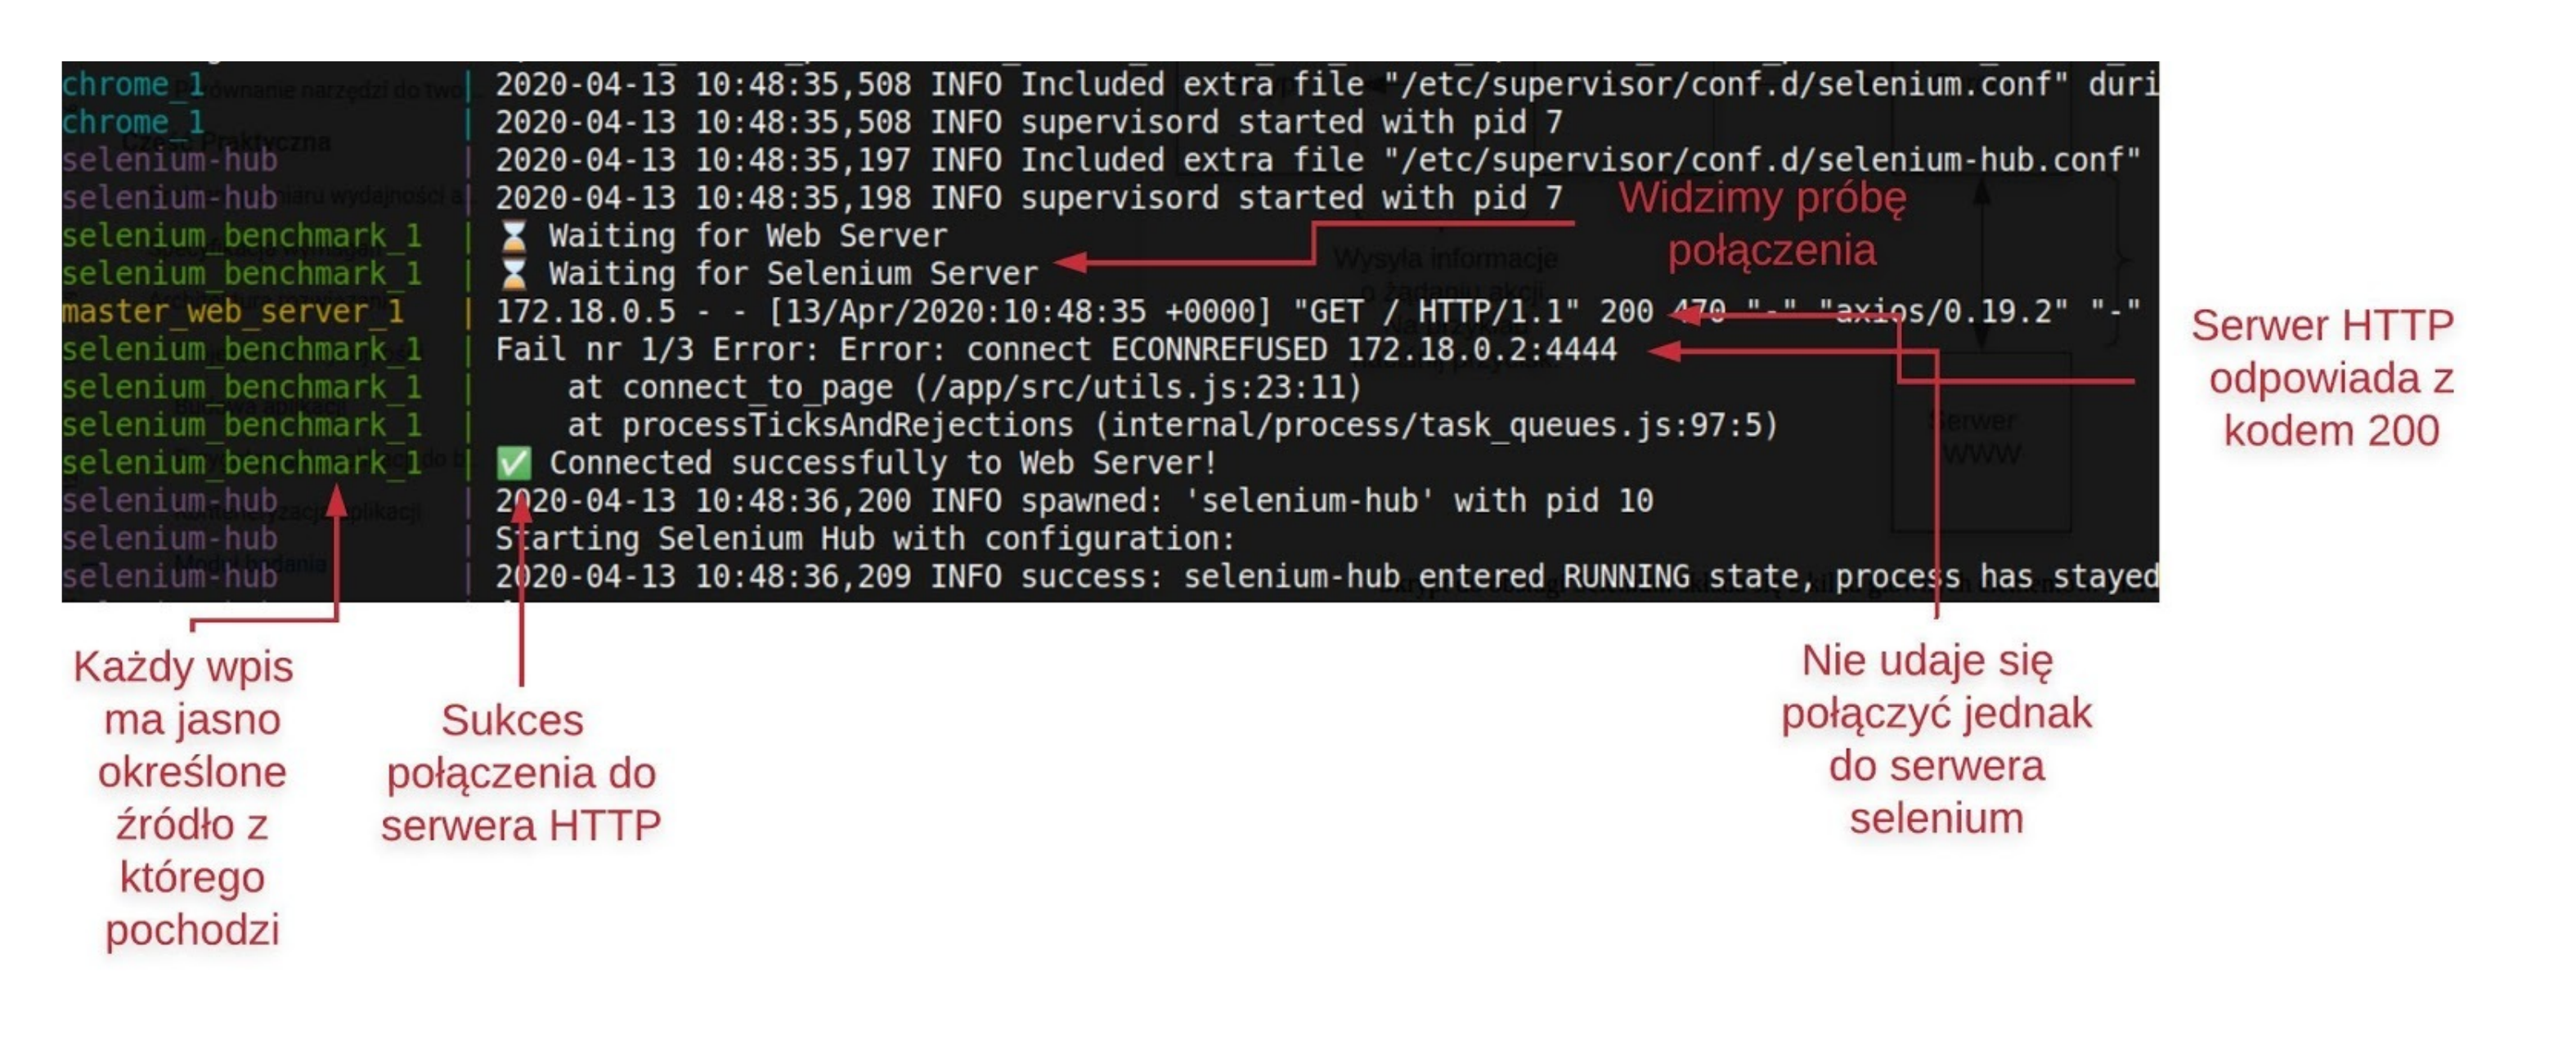
\includegraphics[width=12cm]{rysunek_25.png}
    \caption{Wycinek skryptu ukazujący uzyskanie połączenia do Selenium pomimo początkowych problemów}
    \label{fig:rysunek_25}
\end{figure}

\begin{figure}[!ht]
    \centering
    \includegraphics[width=12cm]{rysunek_26.png}
    \caption{Grafika przedstawia rozpoczęcie badania}
    \label{fig:rysunek_26}
\end{figure}

\begin{figure}[!ht]
    \centering
    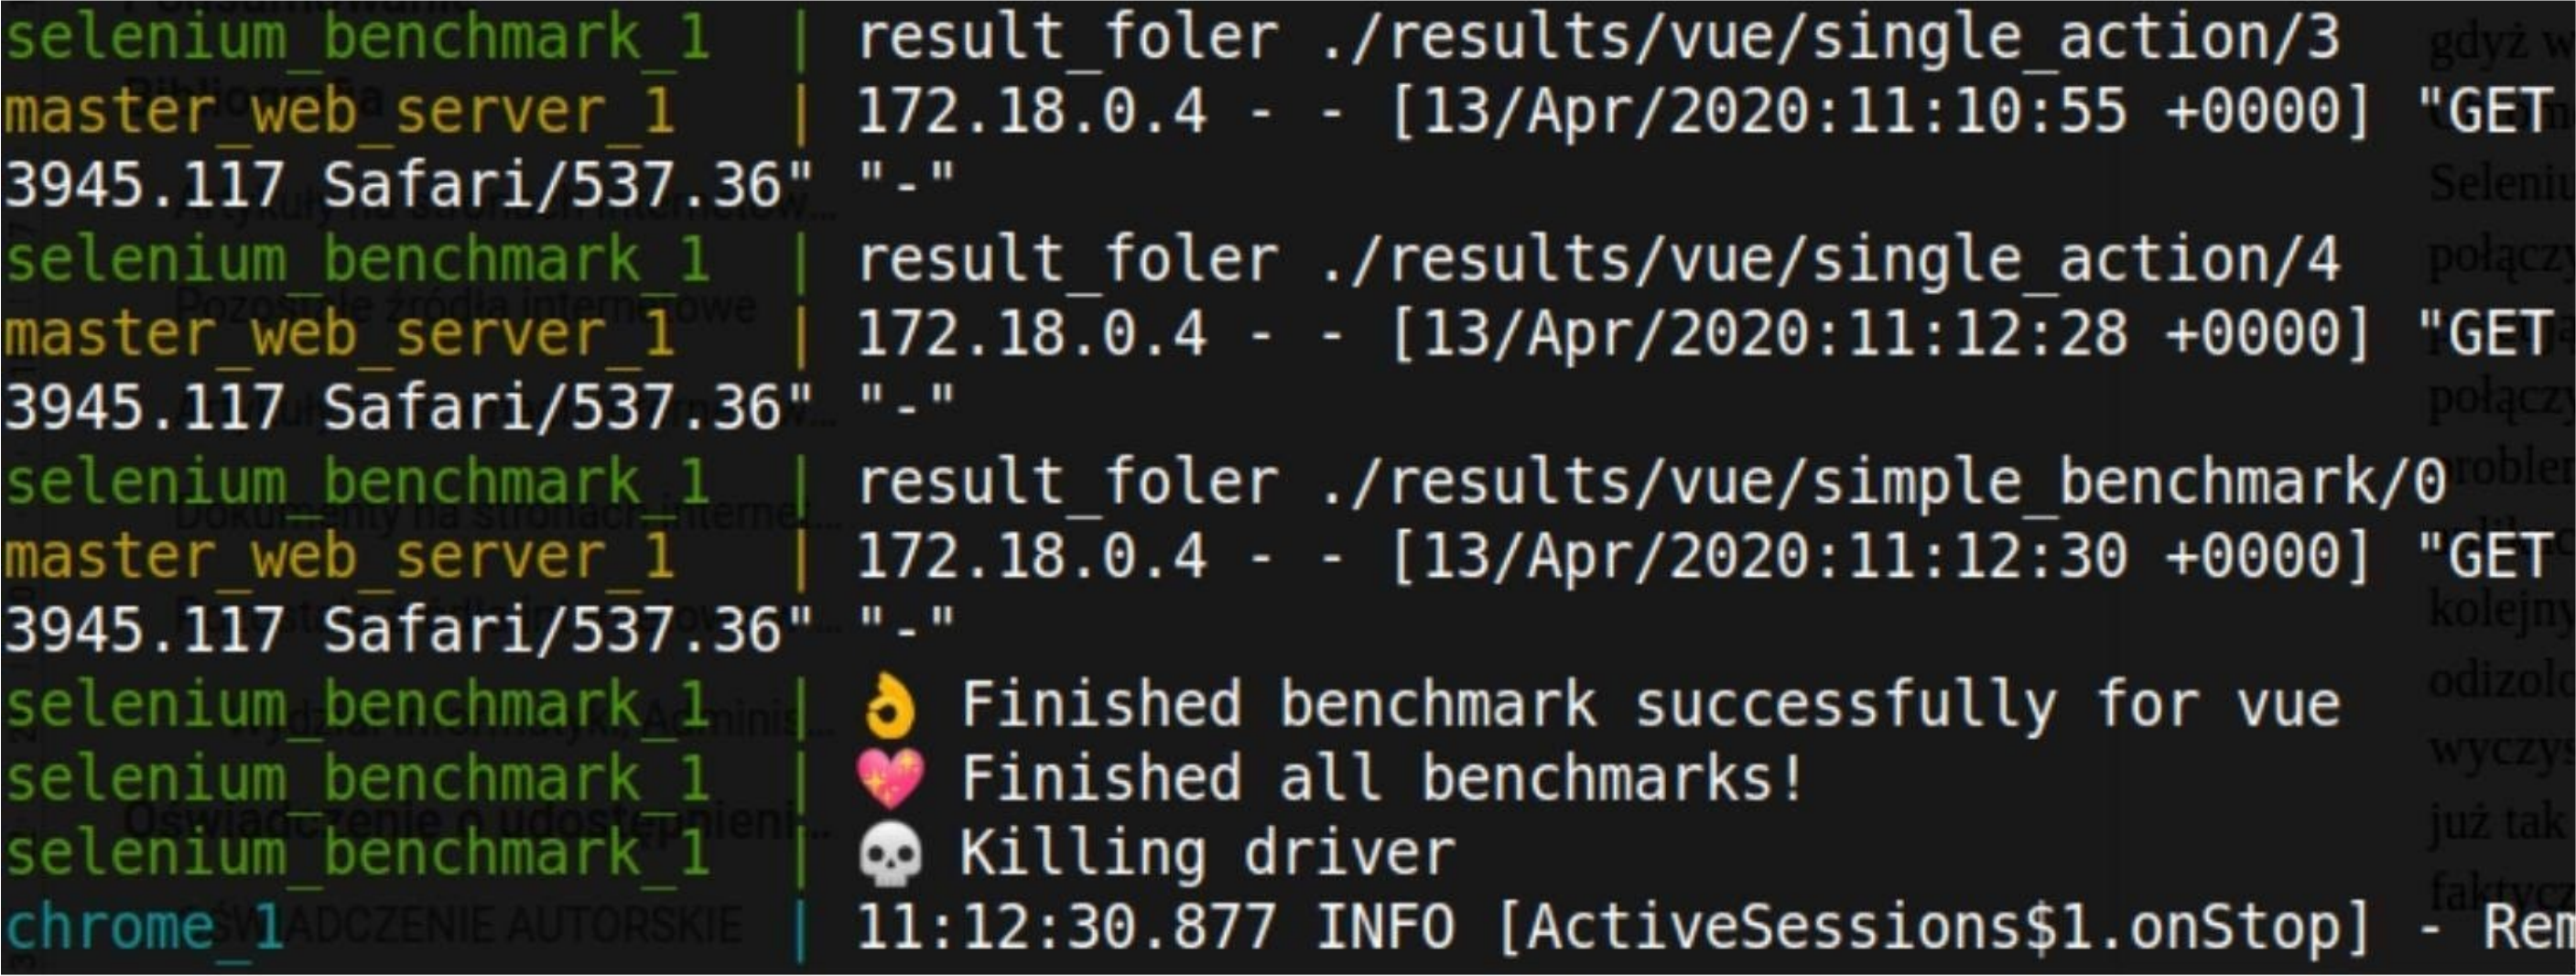
\includegraphics[width=12cm]{rysunek_27.png}
    \caption{Grafika przedstawia skrypt zakańczający badanie po zapisaniu zebranych danych na dysk - widzimy, że ważnym elementem jest zamknięcie połączenia do Selenium}
    \label{fig:rysunek_27}
\end{figure}

\begin{figure}[!ht]
    \centering
    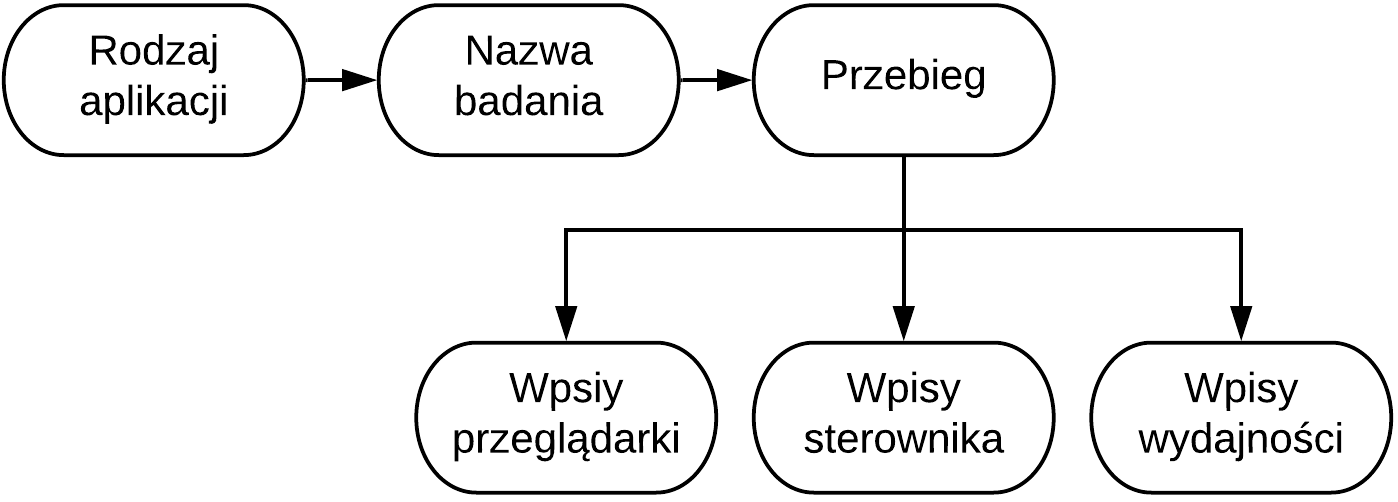
\includegraphics[width=12cm]{rysunek_28.png}
    \caption{Ilustracja struktury wyniku badania na które zostanie poddane dalszej obróbce}
    \label{fig:rysunek_28}
\end{figure}

\begin{figure}[!ht]
    \centering
    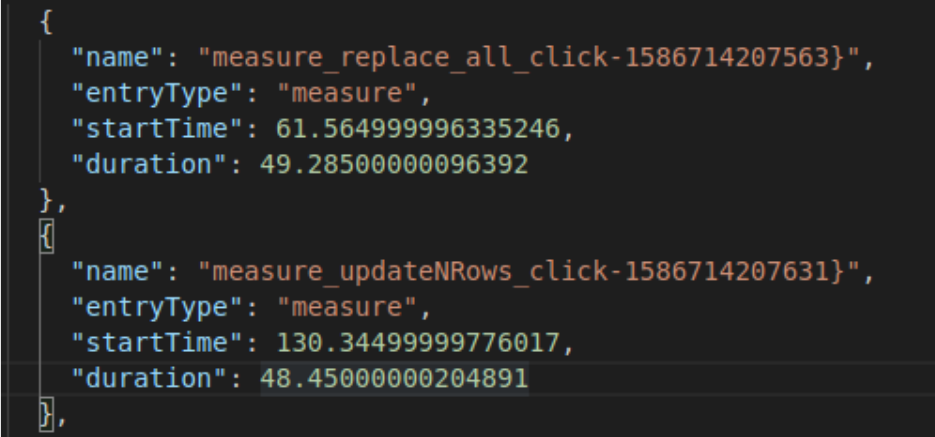
\includegraphics[width=12cm]{rysunek_29.png}
    \caption{Grafika przedstawiająca wpis zebranego pomiaru}
    \label{fig:rysunek_29}
\end{figure}

\begin{figure}[!ht]
    \centering
    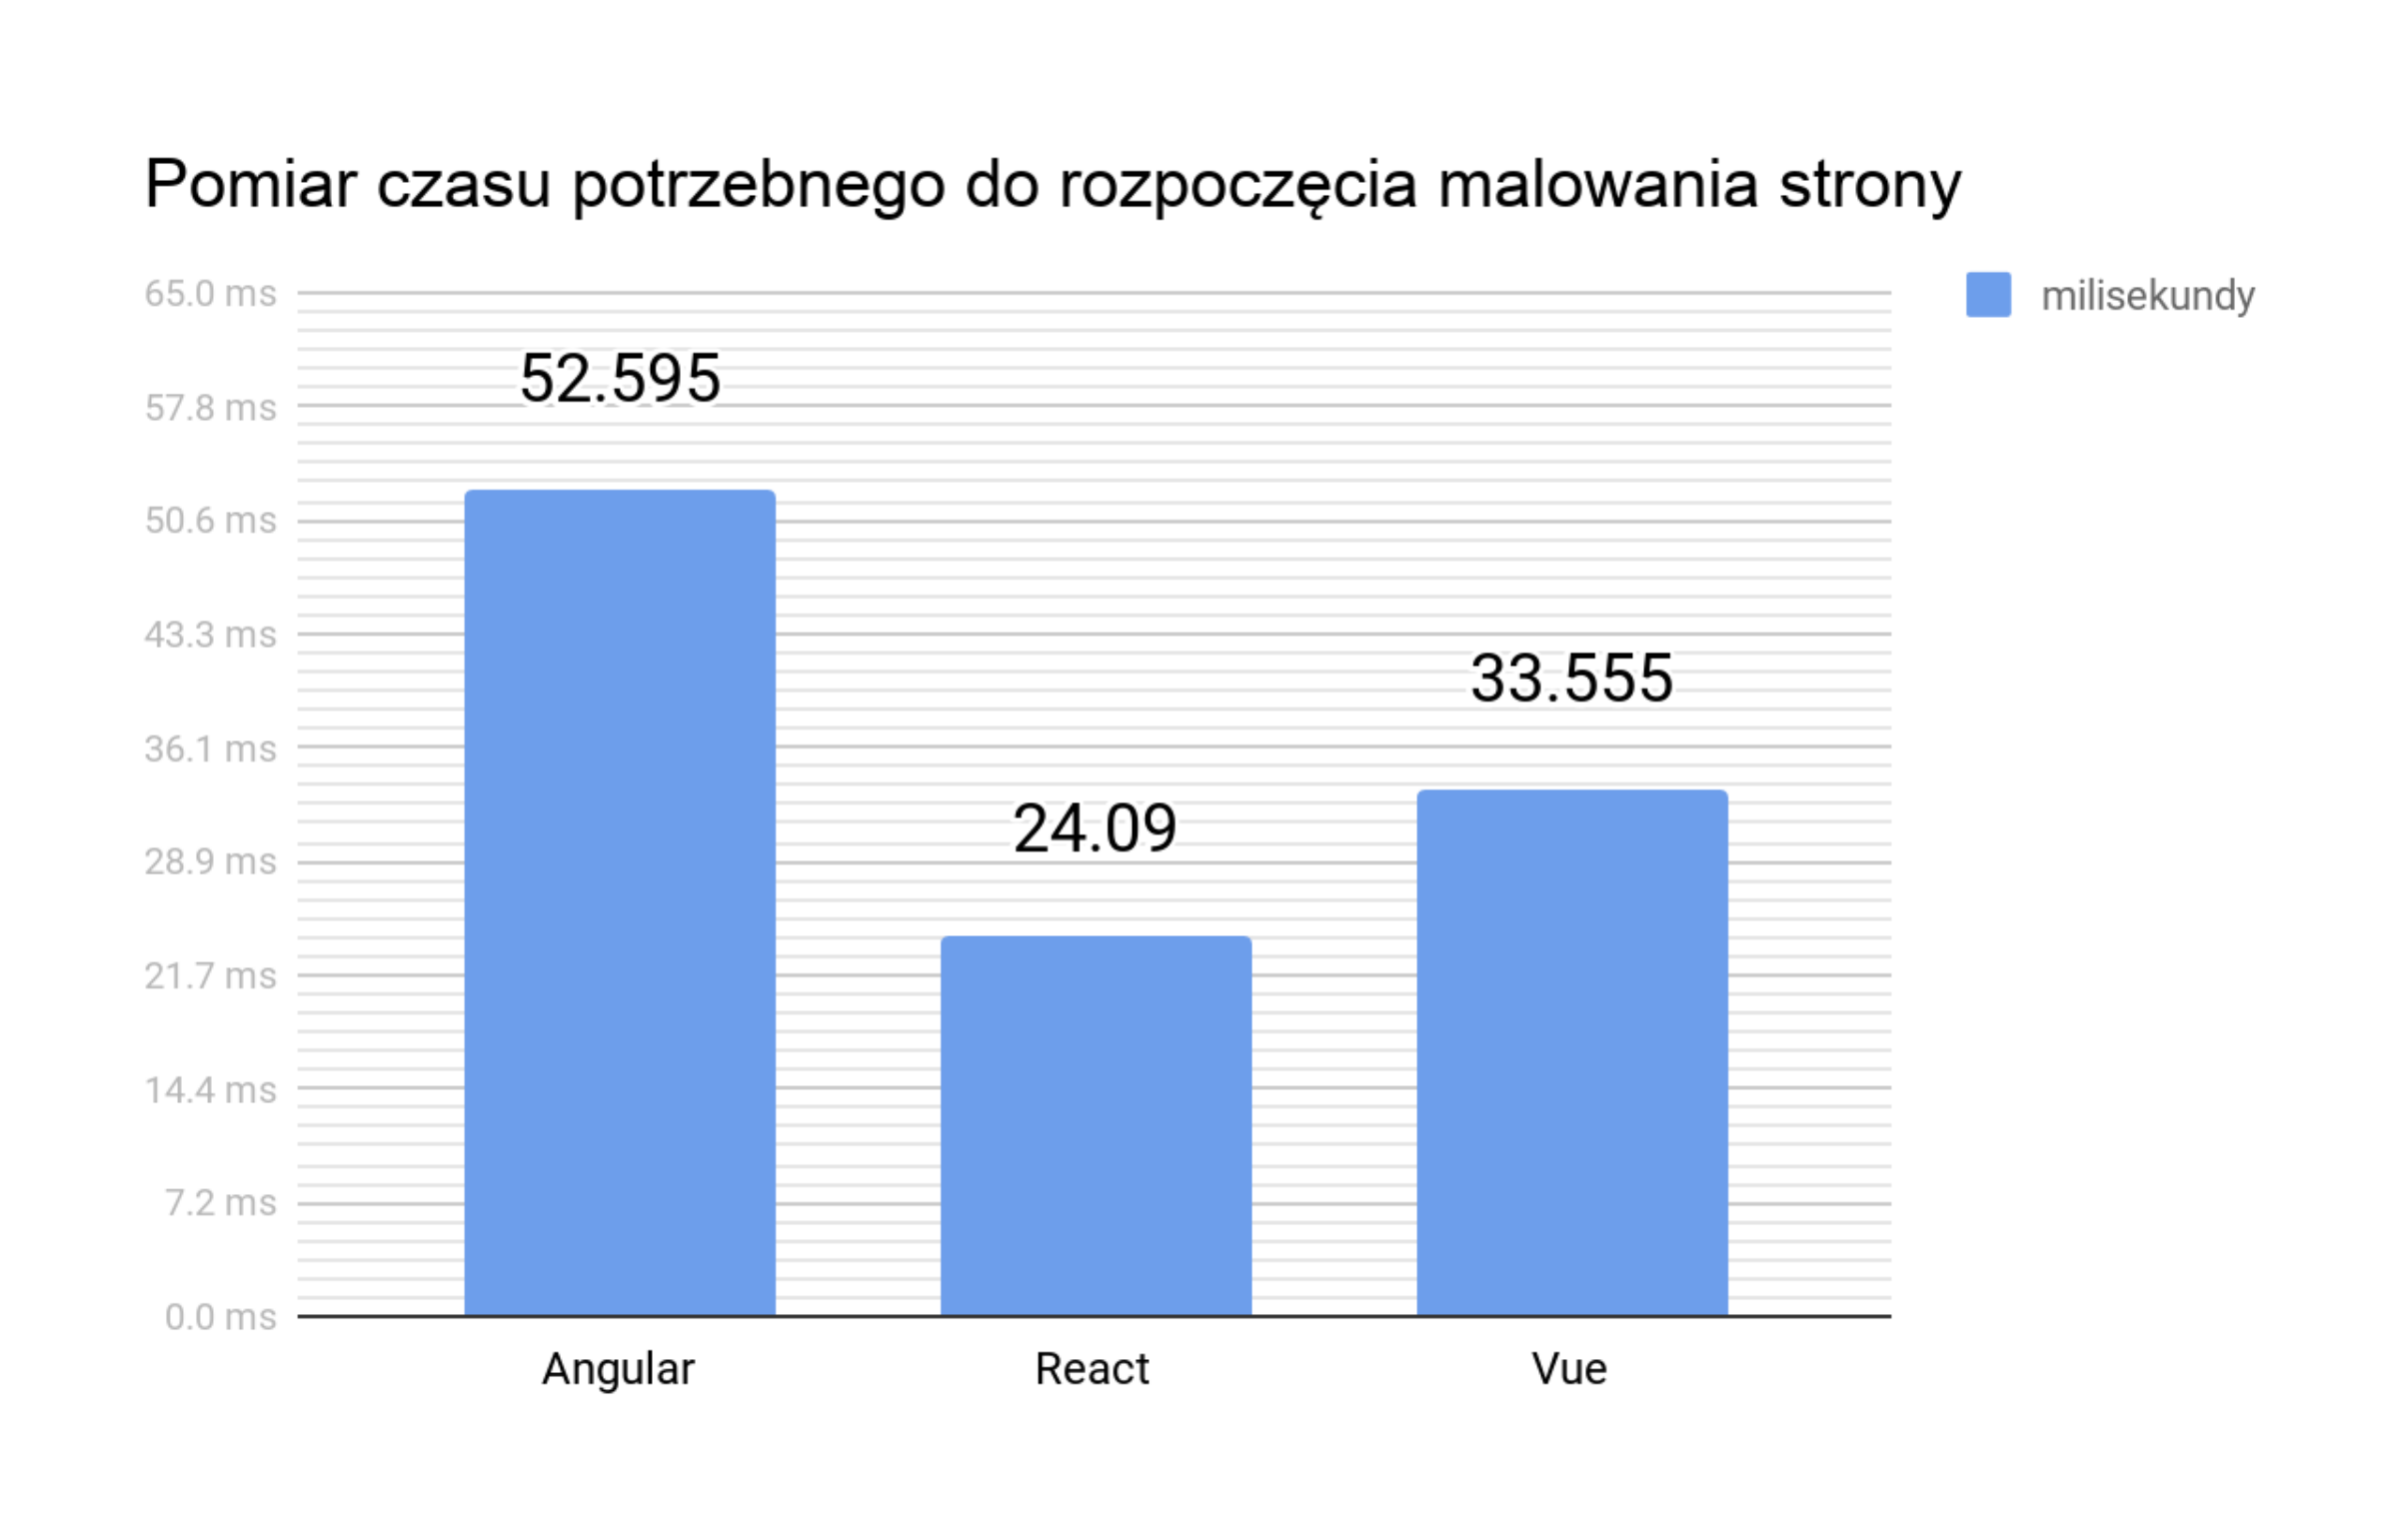
\includegraphics[width=12cm]{rysunek_30.png}
    \caption{Diagram kolumnowy ukazujący wynik badania czasu potrzebnego do rozpoczęcia malowania strony}
    \label{fig:rysunek_30}
\end{figure}

\begin{figure}[!ht]
    \centering
    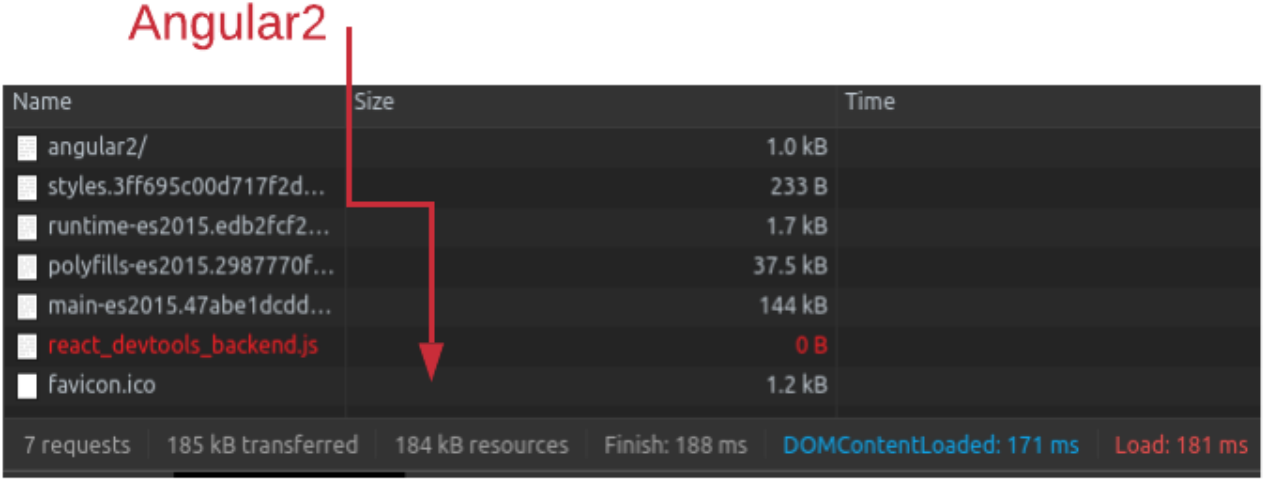
\includegraphics[width=12cm]{rysunek_31.png}
    \caption{Grafika ukazująca rozmiar plików zasobów dla aplikacji Angular2}
    \label{fig:rysunek_31}
\end{figure}

\begin{figure}[!ht]
    \centering
    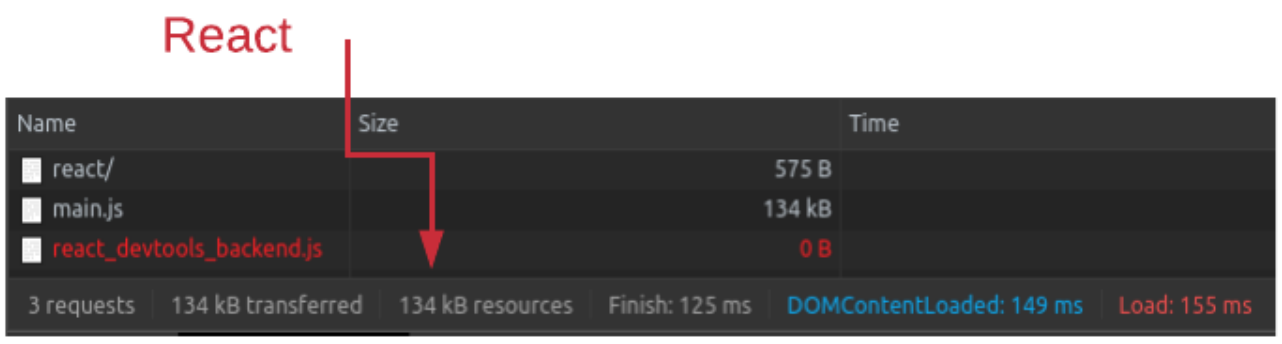
\includegraphics[width=12cm]{rysunek_32.png}
    \caption{Grafika ukazująca rozmiar plików zasobów dla aplikacji React}
    \label{fig:rysunek_32}
\end{figure}

\begin{figure}[!ht]
    \centering
    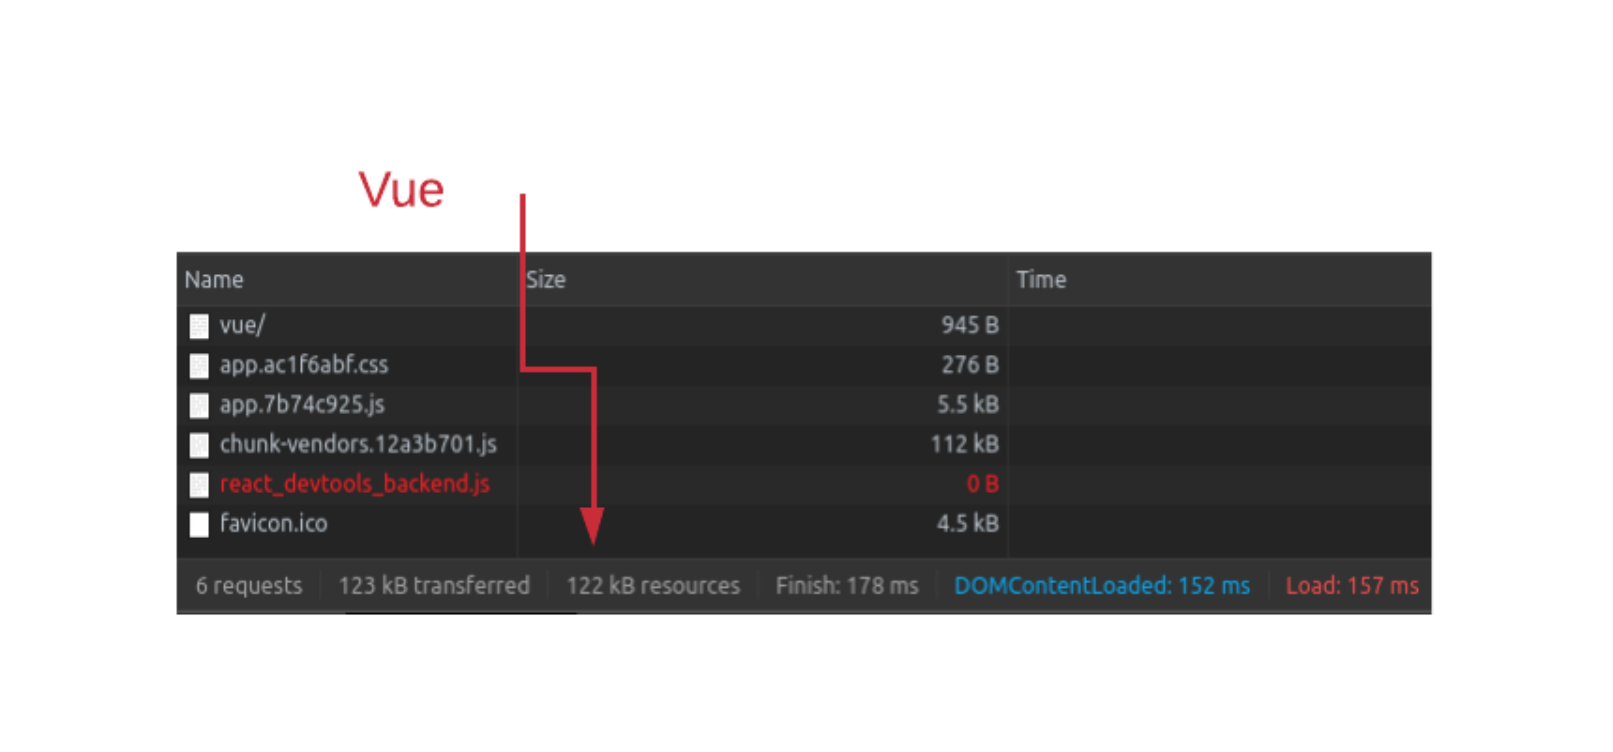
\includegraphics[width=12cm]{rysunek_33.png}
    \caption{Grafika ukazująca rozmiar plików zasobów dla aplikacji Vue}
    \label{fig:rysunek_33}
\end{figure}

\begin{figure}[!ht]
    \centering
    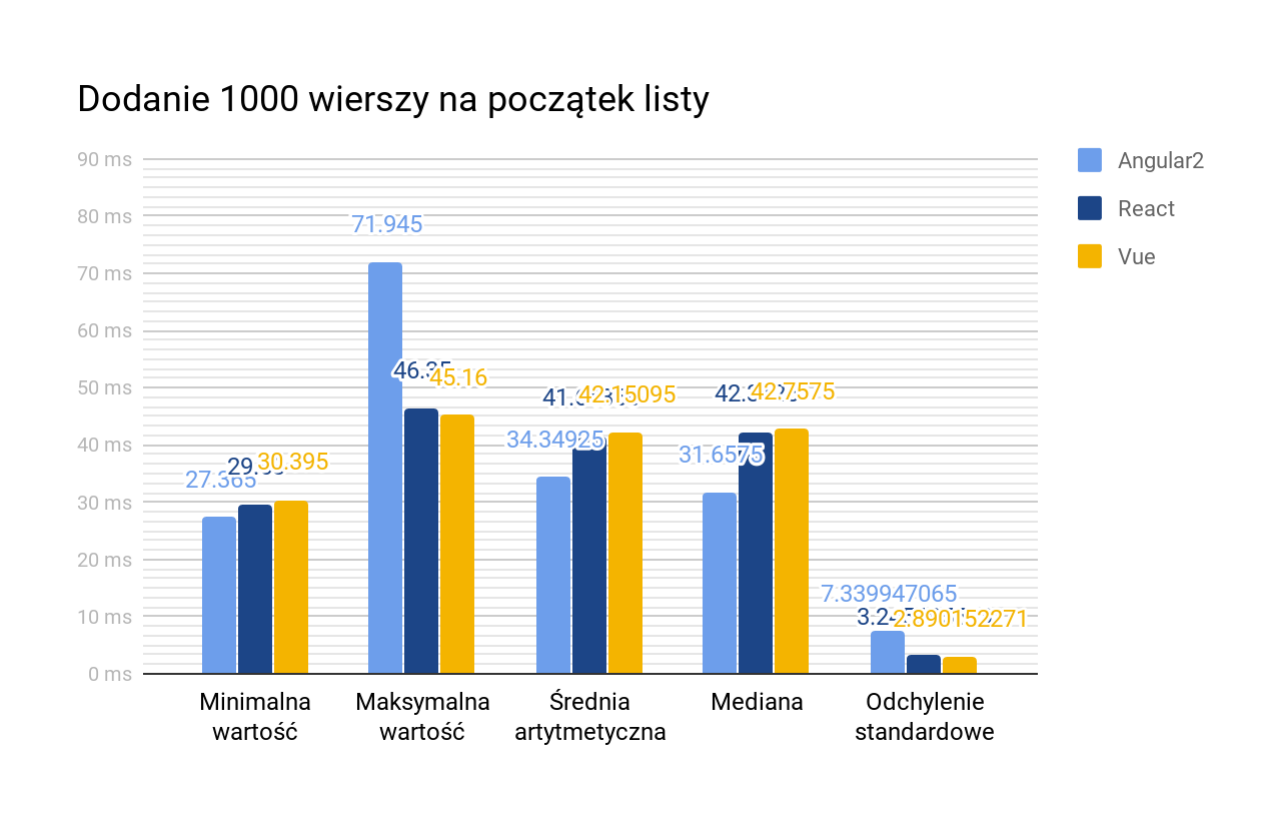
\includegraphics[width=12cm]{rysunek_34.png}
    \caption{Diagram kolumnowy obrazujący wynik badania pomiaru czasu dodania 1000 elementów na początek listy}
    \label{fig:rysunek_34}
\end{figure}

\begin{figure}[!ht]
    \centering
    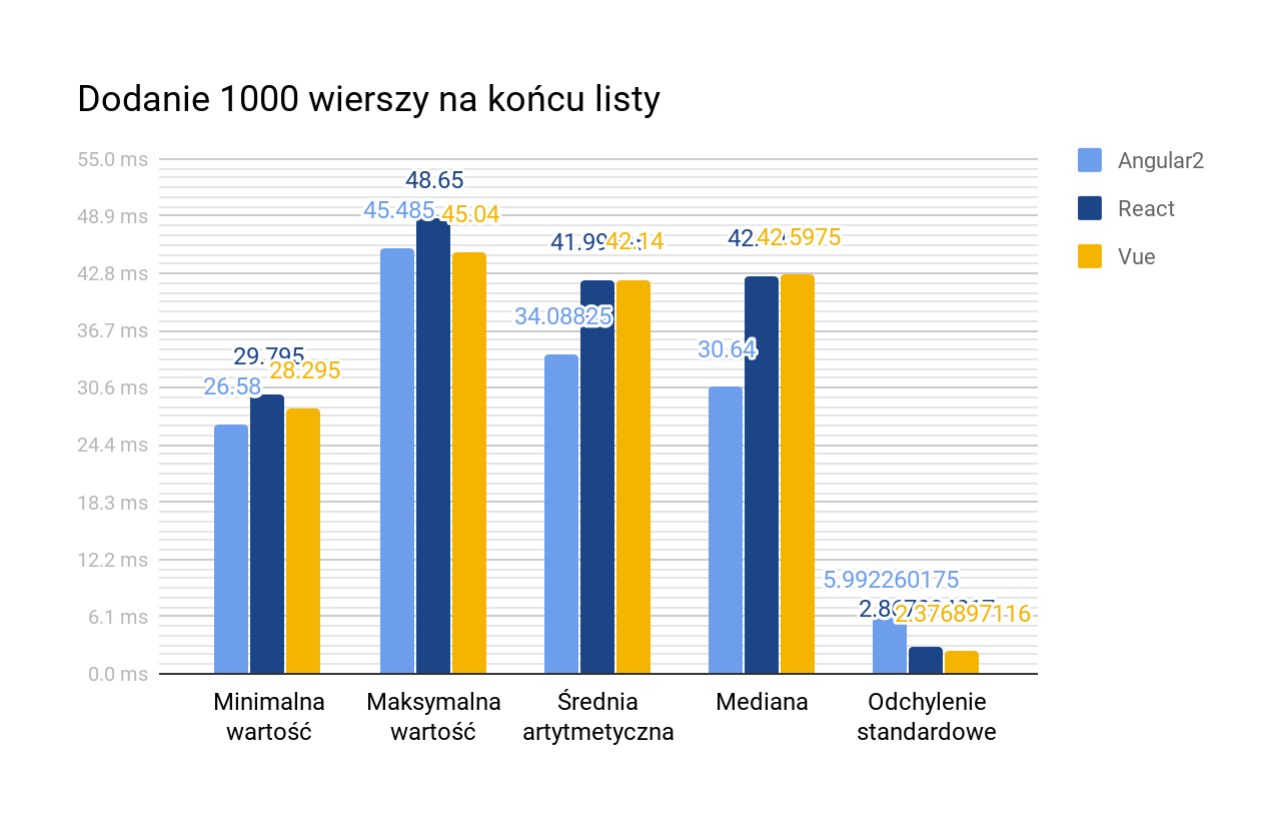
\includegraphics[width=12cm]{rysunek_35.png}
    \caption{Diagram kolumnowy obrazujący wynik badania pomiaru czasu dodania 1000 elementów na koniec listy}
    \label{fig:rysunek_35}
\end{figure}

\begin{figure}[!ht]
    \centering
    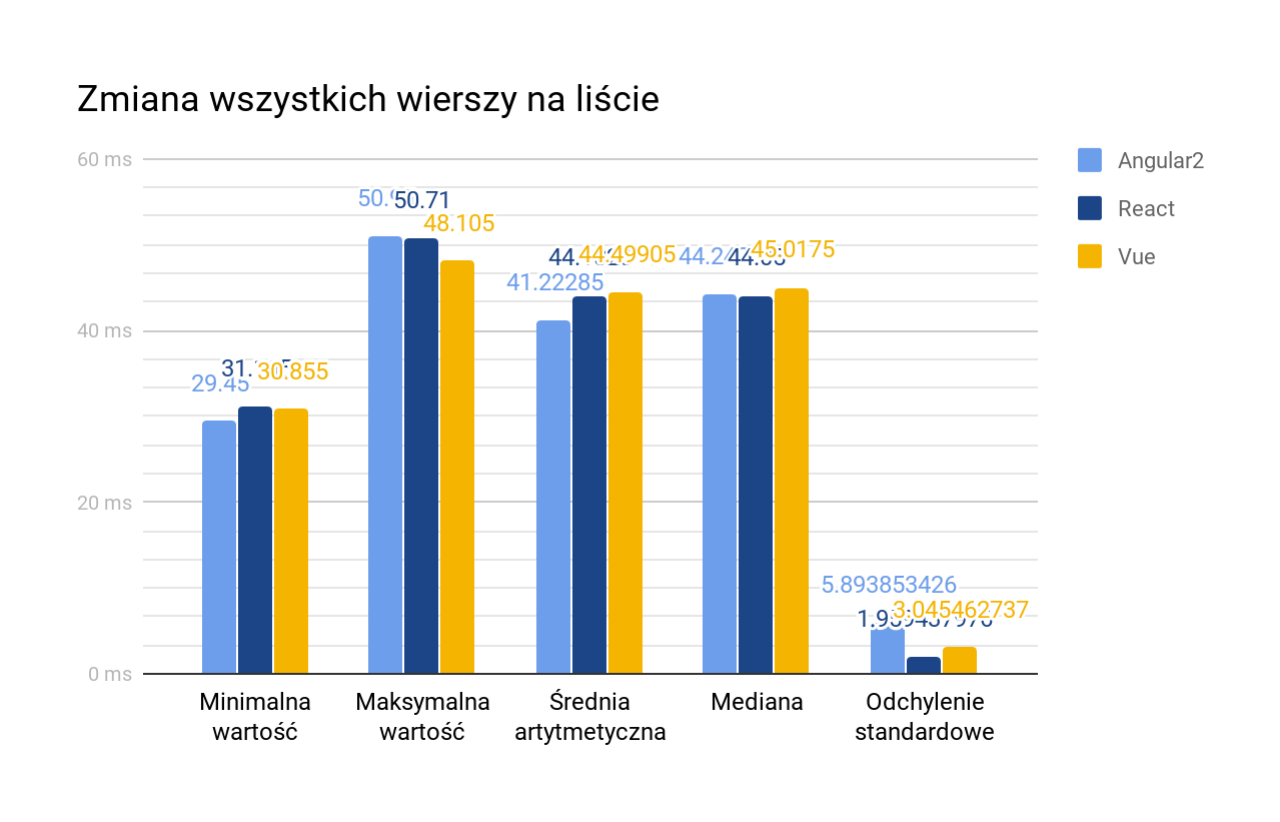
\includegraphics[width=12cm]{rysunek_36.png}
    \caption{Diagram kolumnowy obrazujący wynik badania pomiaru czasu zmiany wszystkich wartości listy dla 1000 elementów}
    \label{fig:rysunek_36}
\end{figure}

\begin{figure}[!ht]
    \centering
    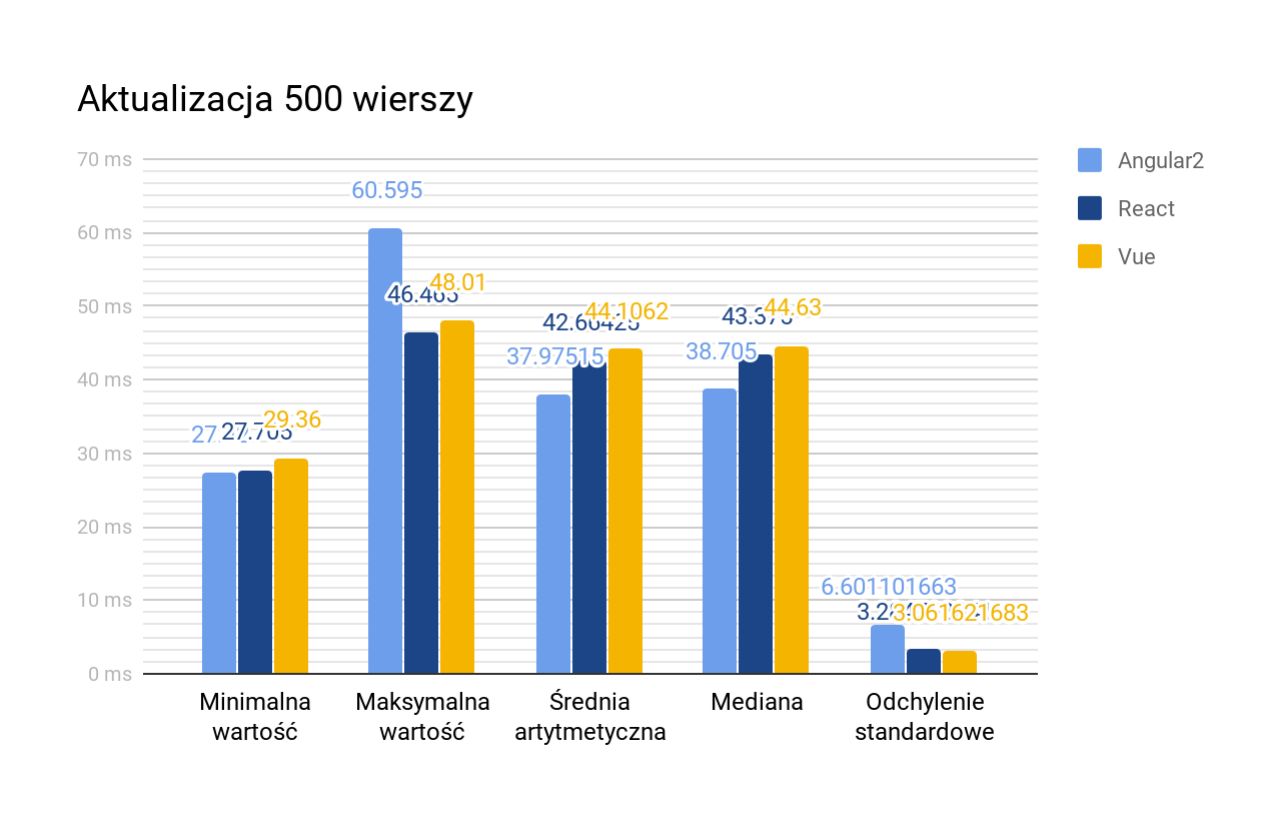
\includegraphics[width=12cm]{rysunek_37.png}
    \caption{Diagram kolumnowy obrazujący wynik badania pomiaru czasu zmiany wartości dla 500 elementów listy}
    \label{fig:rysunek_37}
\end{figure}

\begin{figure}[!ht]
    \centering
    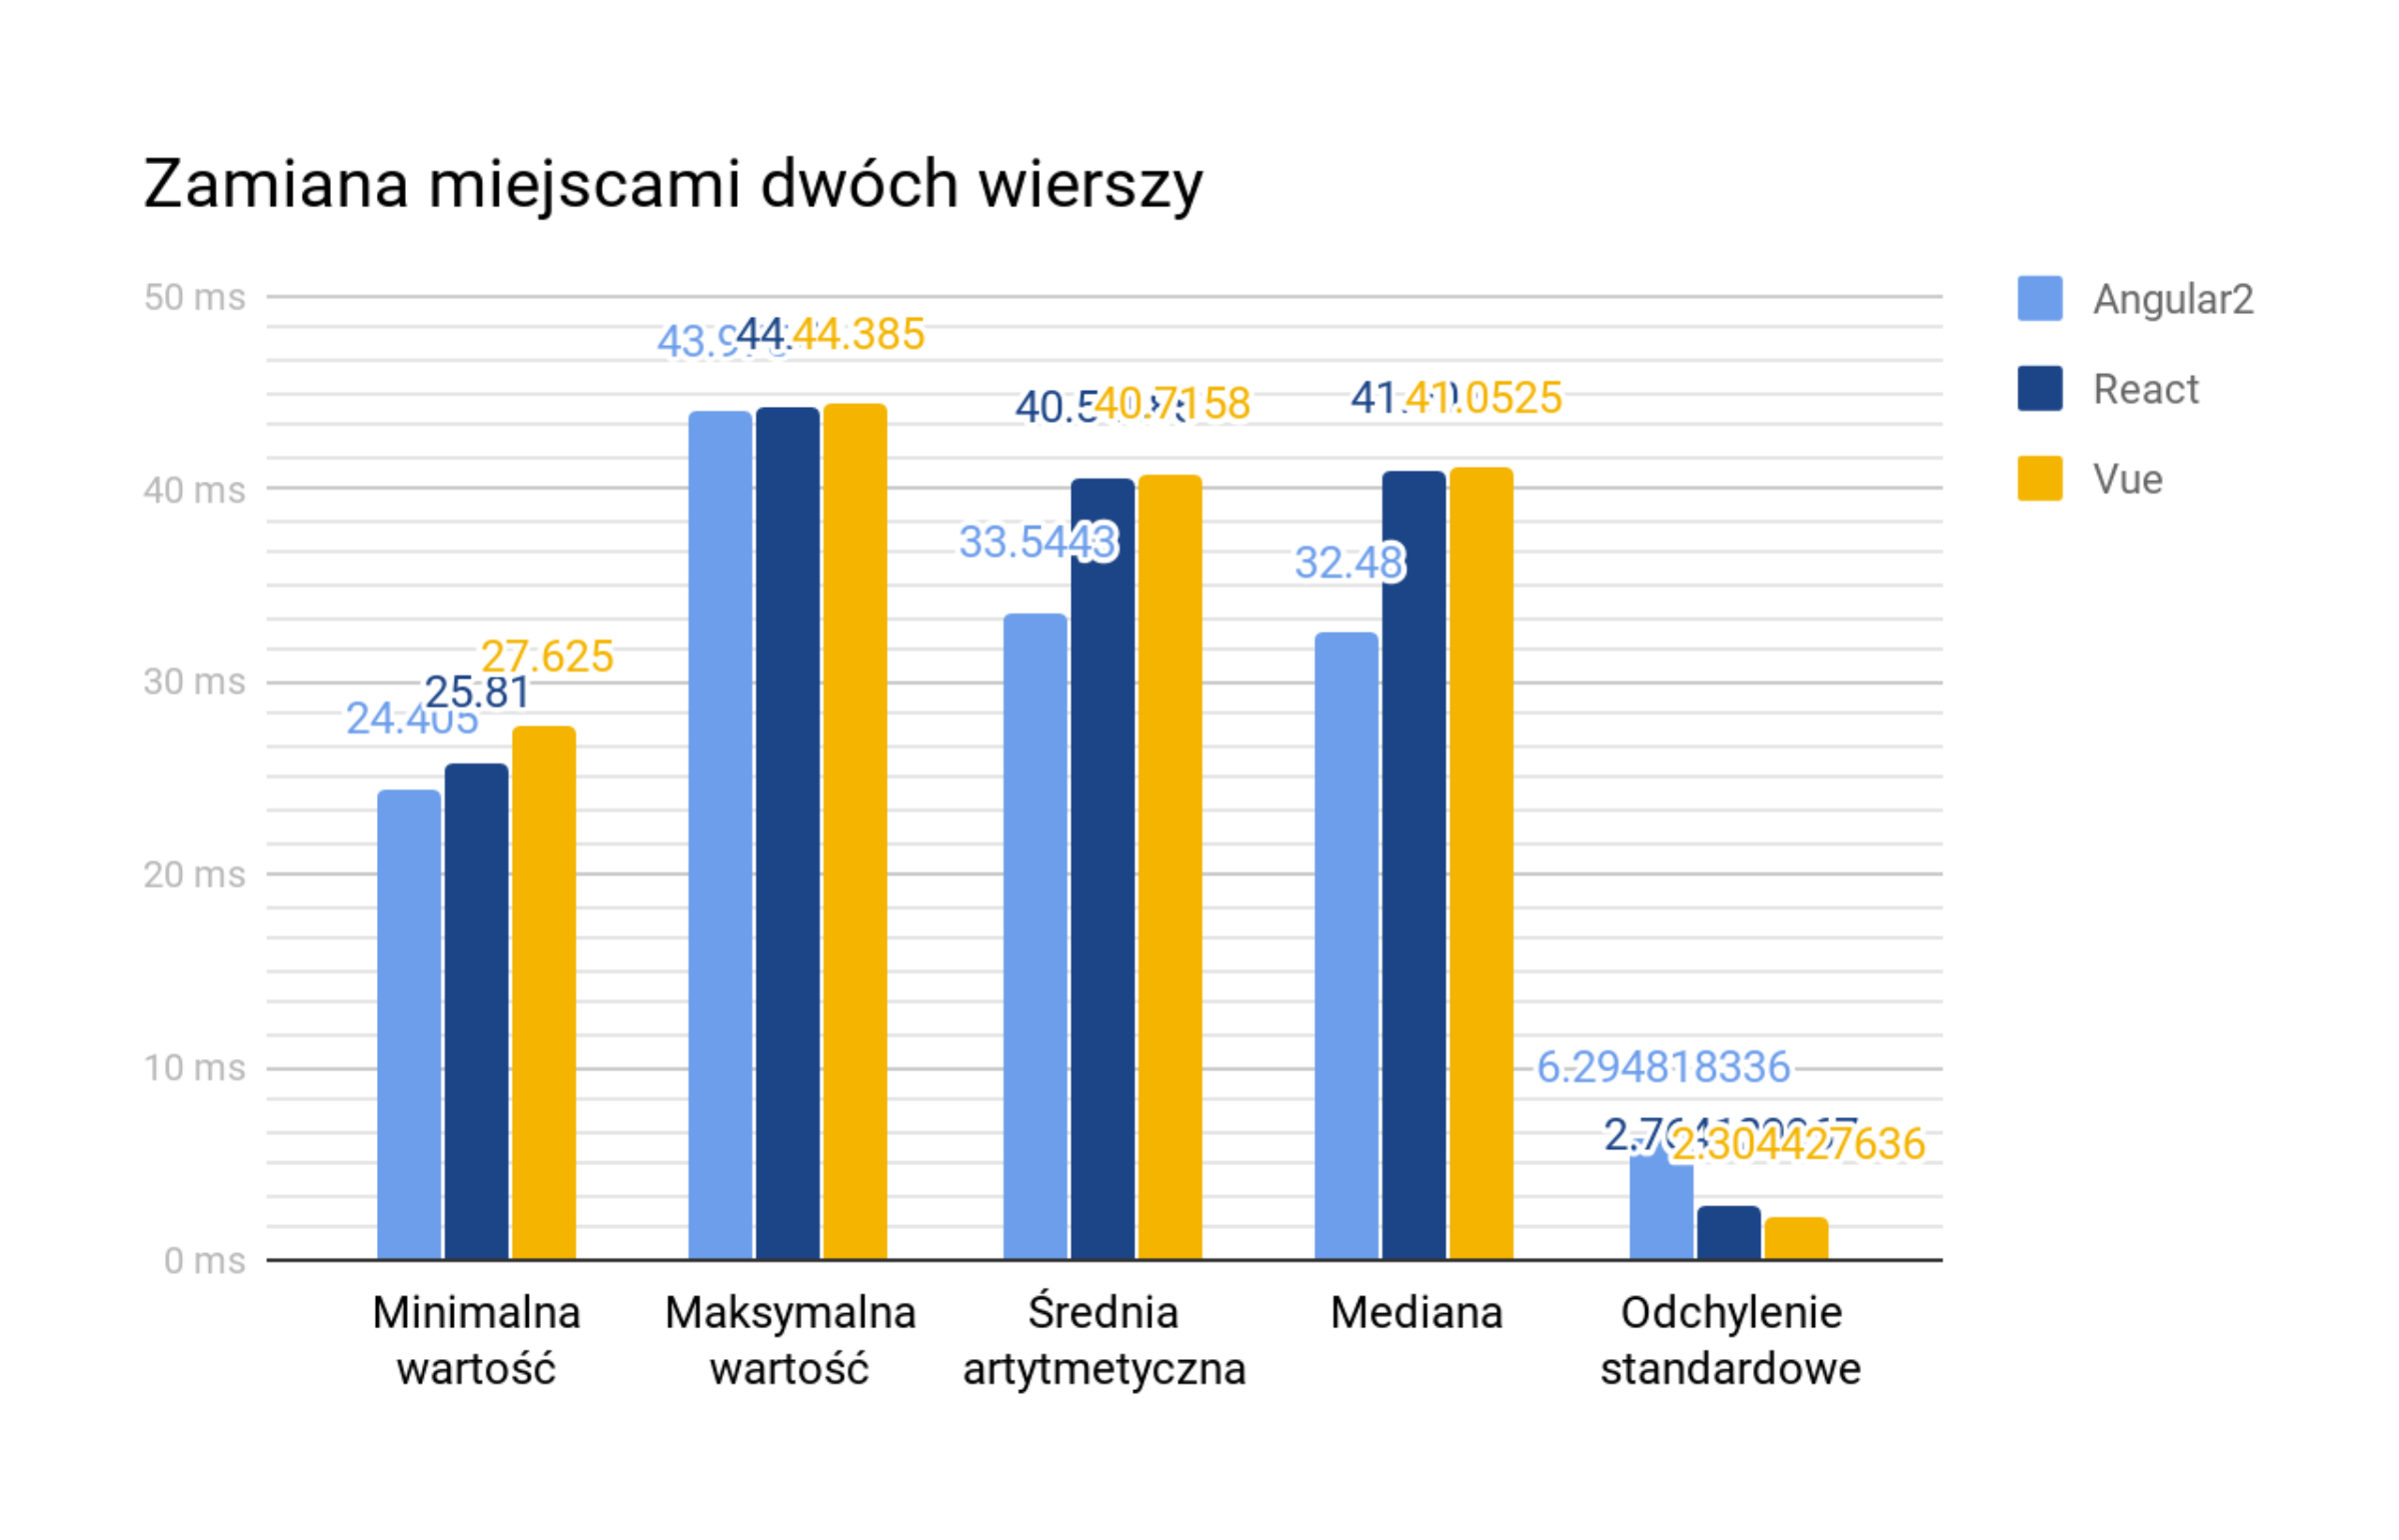
\includegraphics[width=12cm]{rysunek_38.png}
    \caption{Diagram kolumnowy obrazujący wynik badania pomiaru czasu zamiany miejscami dwóch wartości na liście elementów}
    \label{fig:rysunek_38}
\end{figure}

\begin{figure}[!ht]
    \centering
    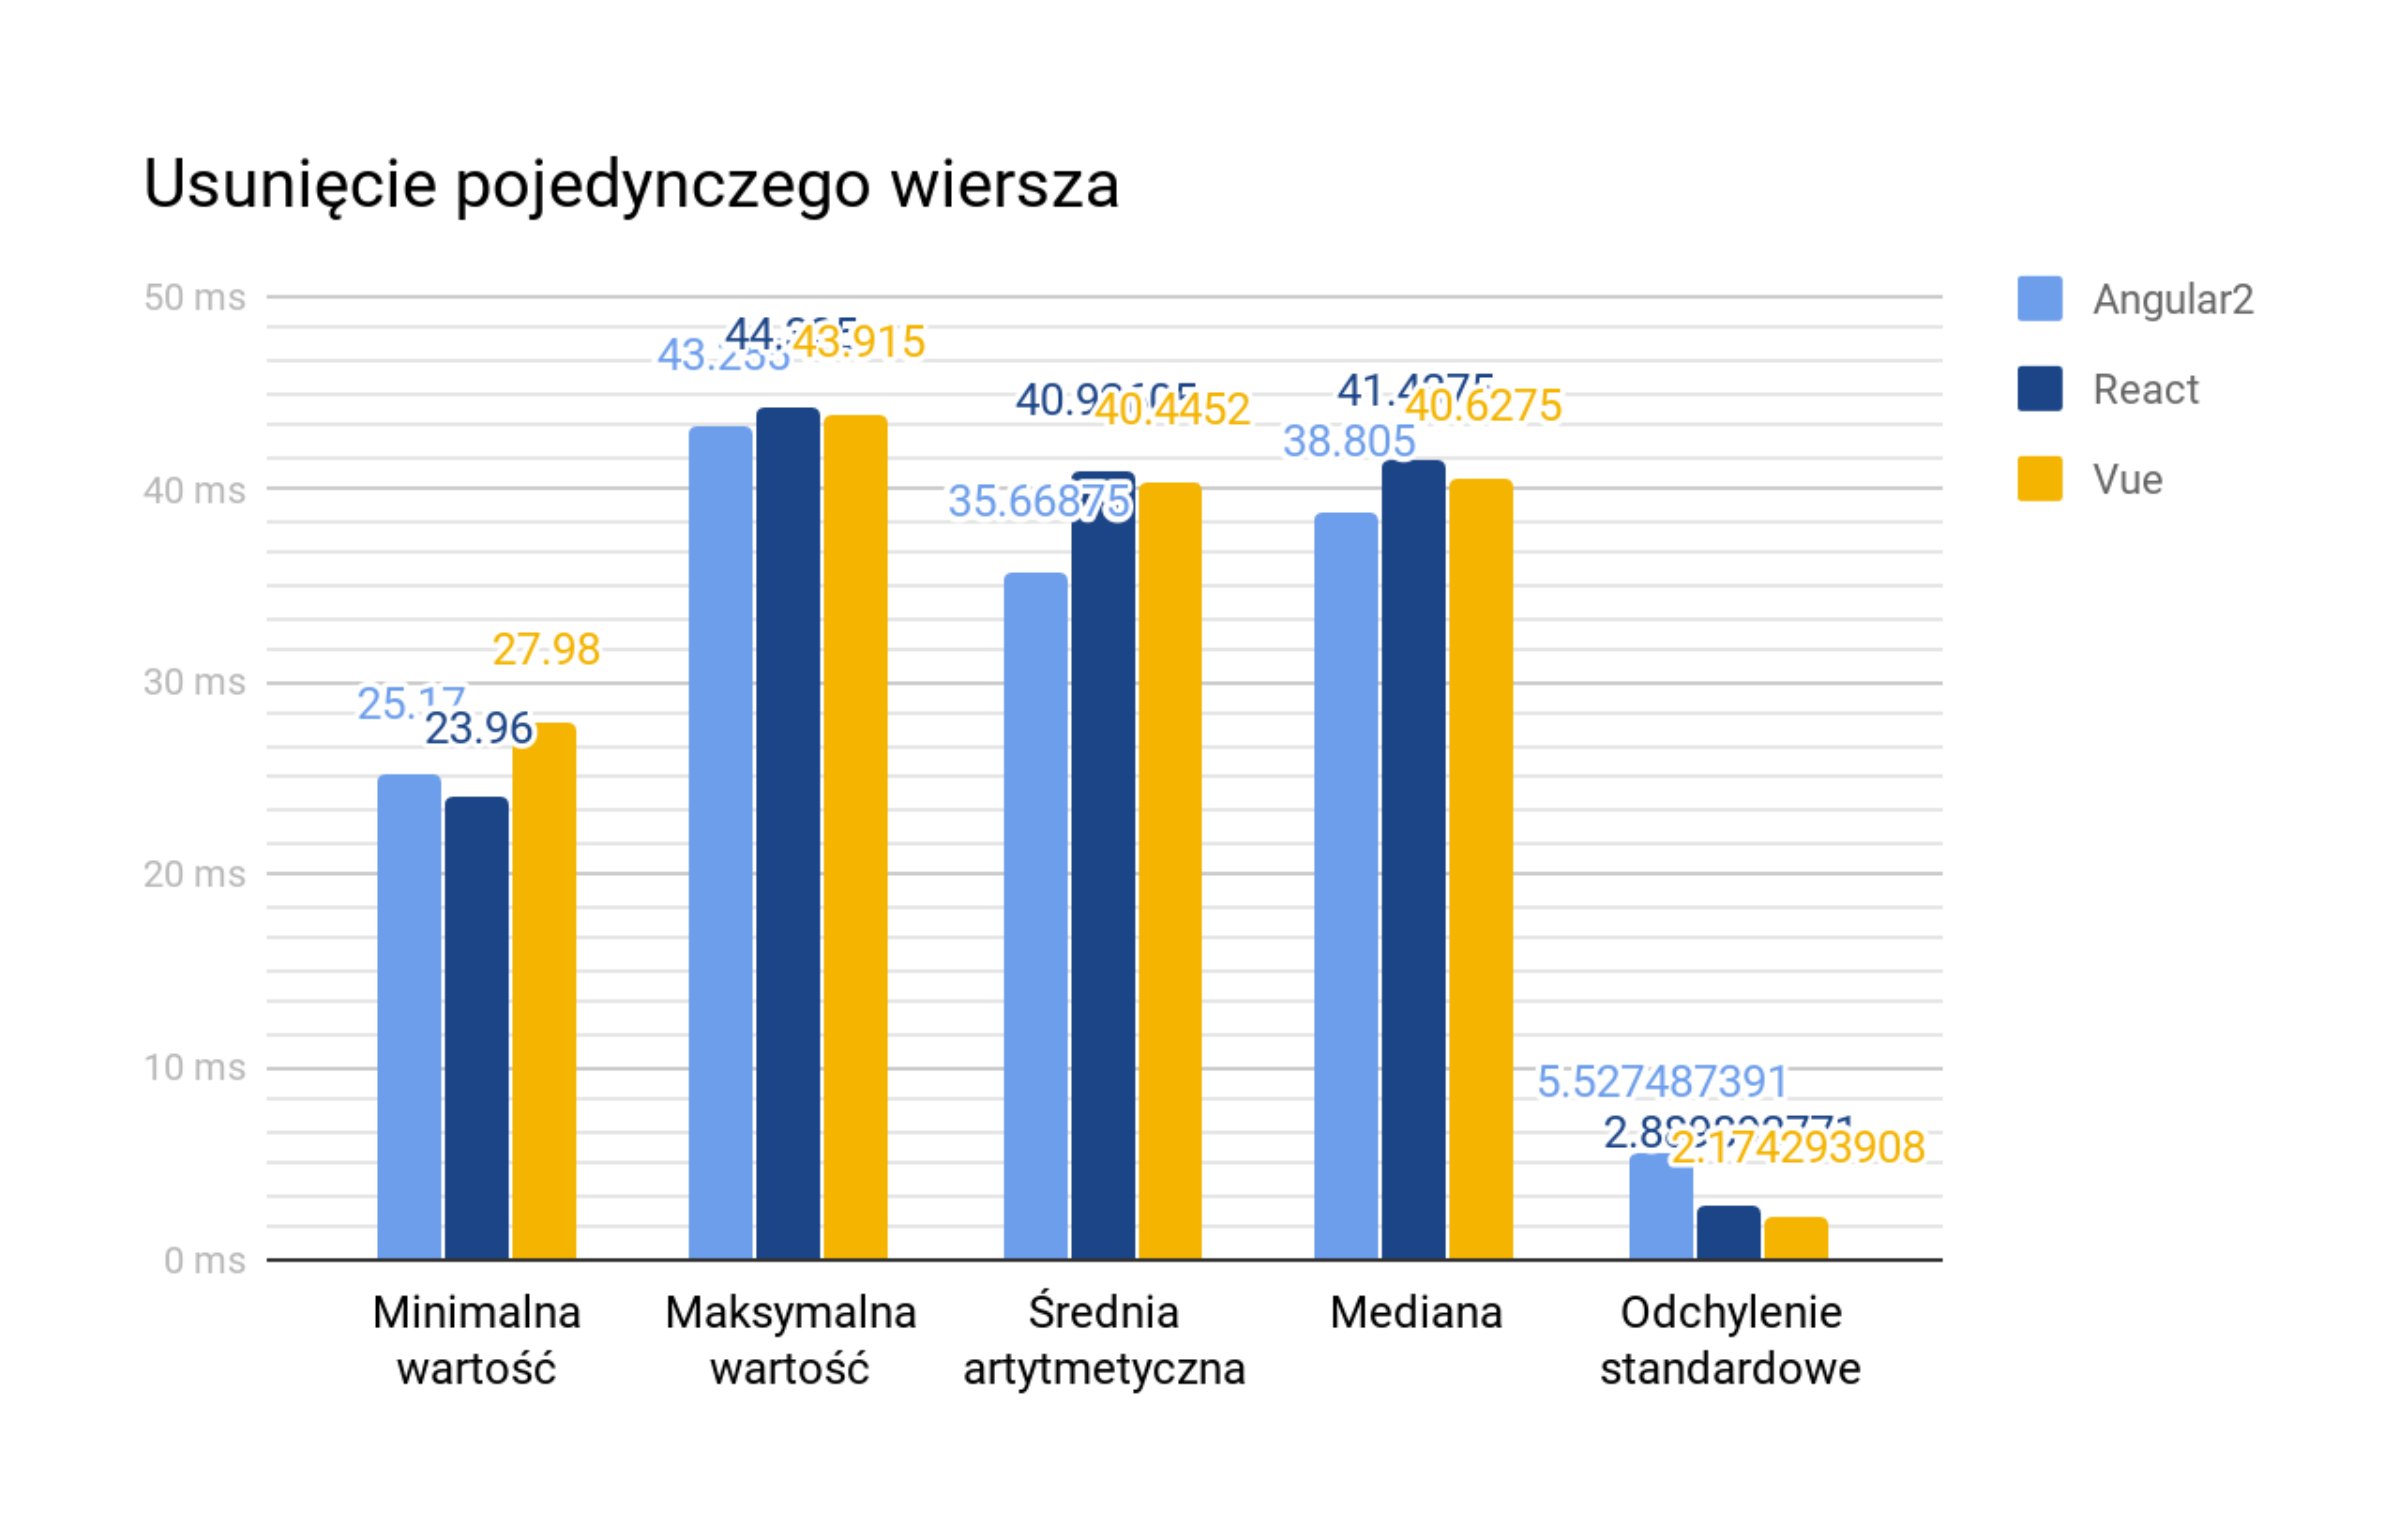
\includegraphics[width=12cm]{rysunek_39.png}
    \caption{Diagram kolumnowy obrazujący wynik badania pomiaru czasu usunięcia pojedynczej wartości z listy elementów}
    \label{fig:rysunek_39}
\end{figure}

\begin{figure}[!ht]
    \centering
    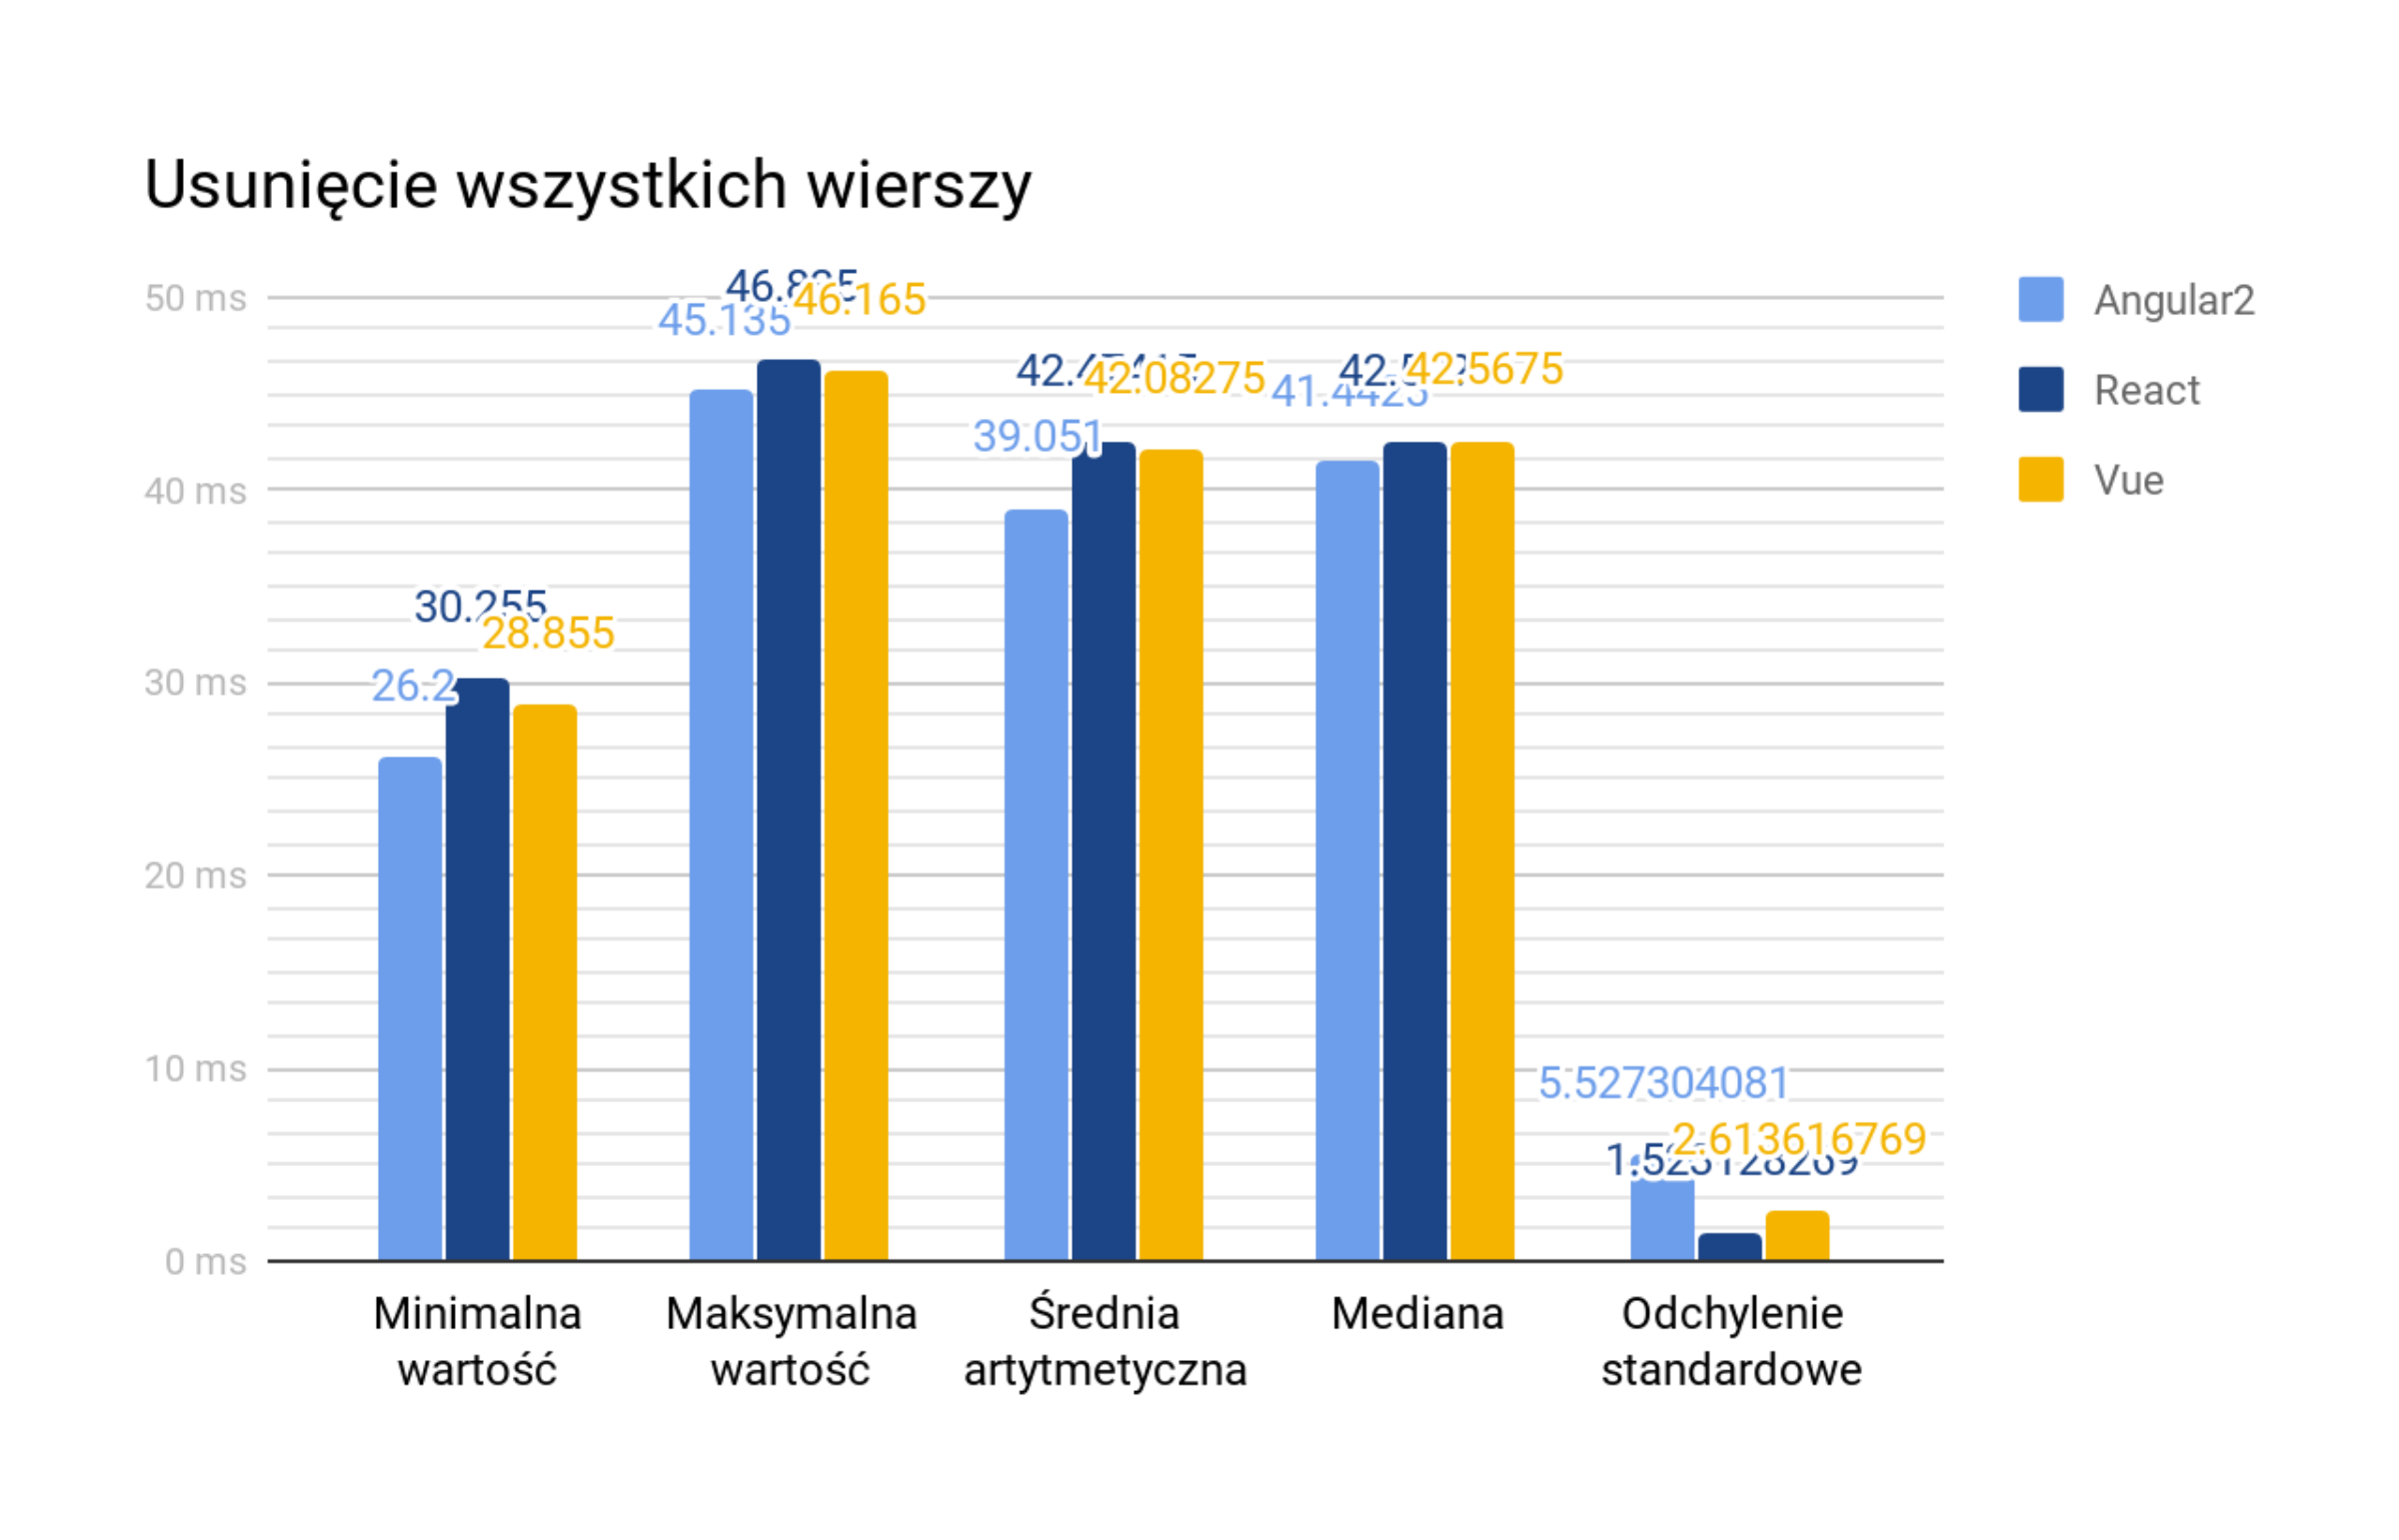
\includegraphics[width=12cm]{rysunek_40.png}
    \caption{Diagram kolumnowy obrazujący wynik badania pomiaru czasu usunięcia wszystkich wartości z listy elementów}
    \label{fig:rysunek_40}
\end{figure}

%czyści puste strony
\let\cleardoublepage\clearpage